% 中文译本（仅供阅读）— Fixed Points and Certified Boundedness of Unrolled Born/Contrast-Source Inverse Scattering Networks
\documentclass[UTF8,a4paper,11pt]{ctexart}

\usepackage{mathtools}
\usepackage{amsmath,amssymb,amsthm}
\usepackage{siunitx}
\usepackage{algorithm}
\usepackage{algpseudocode}
\usepackage{booktabs}
\usepackage{multirow}
\usepackage{graphicx}
\usepackage{xcolor}
\usepackage[hidelinks]{hyperref}
\providecommand{\decibel}{dB}

\newcommand{\R}{\mathbb{R}}
\newcommand{\C}{\mathbb{C}}
\newcommand{\norm}[1]{\lVert #1 \rVert}
\newcommand{\infn}[1]{\lVert #1 \rVert_{\infty}}
\newcommand{\mean}{\operatorname{mean}}
\newcommand{\numv}[1]{#1}
\newcommand{\chimax}{0.50}
\newcommand{\epsbar}{0.03}
\newcommand{\gbnorm}{1.6606}
\newcommand{\betacert}{0.8303}
\newcommand{\NumGammaW}{0.915}
\newcommand{\NumClassOne}{0.4037}
\newcommand{\NumClassBest}{0.4037}
\newcommand{\NumClassBestK}{1}
\newcommand{\NumClassEight}{0.4055}
\newcommand{\NumClassHundred}{0.4055}
\newcommand{\NumConsTwo}{0.3913}
\newcommand{\NumConsBest}{0.3716}
\newcommand{\NumConsBestK}{24}
\newcommand{\NumConsEight}{0.3731}
\newcommand{\NumUncBest}{0.3411}
\newcommand{\NumUncBestK}{8}
\newcommand{\NumUncEight}{0.3411}
\newcommand{\NumPriceDelta}{0.032}
\newcommand{\NumPriceDeltaLo}{0.025}
\newcommand{\NumPriceDeltaHi}{0.032}
\newcommand{\NumPriceBudget}{0.0295}
\newcommand{\NumPriceProjUnc}{0.0067}
\newcommand{\NumPriceProjCons}{0.0109}
\newcommand{\NumFrBaseDsmRreLo}{0.821}
\newcommand{\NumFrBaseDsmRreHi}{0.889}
\newcommand{\NumFrBaseDsmResLo}{0.647}
\newcommand{\NumFrBaseDsmResHi}{0.691}
\newcommand{\NumFrBaseDsmPeakHi}{0.17}
\newcommand{\NumFrBaseBornRreLo}{1.061}
\newcommand{\NumFrBaseBornRreHi}{2.173}
\newcommand{\NumFrBaseBornResHi}{0.779}
\newcommand{\NumFrKernRreLo}{1.035}
\newcommand{\NumFrKernRreHi}{1.092}
\newcommand{\NumFrKernResLo}{0.086}
\newcommand{\NumFrKernResHi}{0.162}
\newcommand{\NumBoxGb}{1.6606}
\newcommand{\NumBoxEdge}{0.6022}
\newcommand{\NumBoxBetaSixty}{0.9964}
\newcommand{\NumBoxBetaEighty}{1.3285}
\newcommand{\NumBoxBetaHundred}{1.6606}
\newcommand{\NumBoxRreConsSixty}{0.3806}
\newcommand{\NumBoxRreConsEighty}{0.3866}
\newcommand{\NumBoxRreConsHundred}{0.3949}
\newcommand{\NumBoxRreUncSixty}{0.3471}
\newcommand{\NumBoxRreUncEighty}{0.3506}
\newcommand{\NumBoxRreUncHundred}{0.3576}
\newcommand{\NumBoxChiConsSixty}{0.600}
\newcommand{\NumBoxChiConsEighty}{0.800}
\newcommand{\NumBoxChiConsHundred}{1.000}
\newcommand{\NumBoxRuns}{6}
\newcommand{\NumDepDeltaArchPct}{-0.56}
\newcommand{\NumDepDeltaUniPct}{0.76}
\newcommand{\NumDepDeltaUncUniPct}{-0.33}
\newcommand{\NumDepUniConsSixteen}{0.36567}
\newcommand{\NumDepUniConsTwentyFour}{0.36846}
\newcommand{\NumDepUniDrift}{\ensuremath{1.1\times10^{-2}}}
\newcommand{\NumDepUniFloor}{\ensuremath{1.8\times10^{-2}}}
\newcommand{\NumDepUniShiftSixteen}{\ensuremath{8.0\times10^{-3}}}
\newcommand{\NumDepUniShiftTwentyFour}{\ensuremath{3.2\times10^{-3}}}
\newcommand{\NumSsimCons}{0.6785}
\newcommand{\NumSsimUnc}{0.7892}
\newcommand{\NumSsimClsEight}{0.3609}
\newcommand{\NumSsimClsFiveZero}{0.3613}
\newcommand{\NumPsnrCons}{17.02}
\newcommand{\NumPsnrUnc}{18.76}
\newcommand{\NumPsnrClsEight}{15.62}
\newcommand{\NumPsnrClsFiveZero}{15.62}
\newcommand{\NumNImg}{4}
\newcommand{\NumRreImgCons}{0.3132}
\newcommand{\NumRreImgUnc}{0.2569}
\newcommand{\NumResConsHead}{0.0529}
\newcommand{\NumResConsEnd}{0.0843}
\newcommand{\NumResConsTrans}{0.1659}
\newcommand{\NumResConsBandLo}{0.0391}
\newcommand{\NumResConsBandHi}{0.1005}
\newcommand{\NumResClsEnd}{0.0003}
\newcommand{\NumSensCons}{0.1617}
\newcommand{\NumSensUnc}{0.1648}
\newcommand{\NumSigMin}{1.132}
\newcommand{\NumSigMax}{5.659}
\newcommand{\NumLipHCons}{0.2503}
\newcommand{\NumLipHUnc}{2.704}
\newcommand{\NumLipRatioUncCons}{10.8}
\newcommand{\NumLipOverEps}{8.3}
\newcommand{\NumGdCompDeltaPct}{+1.2}
\newcommand{\NumPhysWBlock}{0.6176}
\newcommand{\NumSigCompCons}{1.736}
\newcommand{\NumSigCompUnc}{2.247}
\newcommand{\NumSigCompLayerCons}{3.161}
\newcommand{\NumSigCompLayerUnc}{3.111}
\newcommand{\NumResUncSpike}{0.290}
\newcommand{\NumAlphaCons}{0.27--0.31}
\newcommand{\NumAlphaUnc}{0.22--0.31}
\newcommand{\NumGradConsOne}{0.00299}
\newcommand{\NumGradUncOne}{0.104}
\newcommand{\NumEbWorst}{0.01}
\newcommand{\NumEbBest}{0.12}
\newcommand{\NumAblClsProjOn}{0.4094}
\newcommand{\NumAblClsChi}{0.500}
\newcommand{\NumAblProjDelta}{0.028}
\newcommand{\NumMeasChiNoProj}{1.522}
\newcommand{\NumBetaMeas}{2.528}
\newcommand{\NumFrzUncOnShort}{0.3411}
\newcommand{\NumFrzUncOn}{0.4011}
\newcommand{\NumFrzUncOffShort}{5.7228}
\newcommand{\NumFrzUncOff}{\ensuremath{\mathrm{div.}}}
\newcommand{\NumFrzUncBreak}{31}
\newcommand{\NumFrzUncOffChi}{46.948}
\newcommand{\NumFrzConsOnShort}{0.3731}
\newcommand{\NumFrzConsOn}{0.3832}
\newcommand{\NumFrzConsOffShort}{0.4948}
\newcommand{\NumFrzConsOff}{0.5249}
\newcommand{\NumFrzConsOffChi}{0.737}
\newcommand{\NumSeedN}{15}
\newcommand{\NumSeedNCons}{5}
\newcommand{\NumSeedNUnc}{5}
\newcommand{\NumSeedNProjOff}{5}
\newcommand{\NumSeedRreSdCons}{0.0017}
\newcommand{\NumSeedRreSdUnc}{0.0036}
\newcommand{\NumSeedRreMeanCons}{0.3725}
\newcommand{\NumSeedRreMeanUnc}{0.3389}
\newcommand{\NumSeedRreMedCons}{0.3728}
\newcommand{\NumSeedRreMedUnc}{0.3390}
\newcommand{\NumSeedRreHiCons}{0.3739}
\newcommand{\NumSeedRreHiUnc}{0.3422}
\newcommand{\NumSeedExMeanCons}{0.3877}
\newcommand{\NumSeedExMeanUnc}{0.4548}
\newcommand{\NumSeedExSdCons}{0.0020}
\newcommand{\NumSeedExSdUnc}{0.0099}
\newcommand{\NumSeedChiConsMax}{0.50}
\newcommand{\NumSeedProjOffBox}{0.85--1.26}
\newcommand{\NumSeedFinite}{15/15}
\newcommand{\NumRepFloorMaxRre}{0.0181}
\newcommand{\NumRepFloorMedRre}{0.0021}
\newcommand{\NumRepFloorMaxExtrap}{0.0346}
\newcommand{\NumRepNShared}{9}
\newcommand{\NumRepFiniteStable}{yes}
\newcommand{\NumRepBoxStable}{yes}
\newcommand{\NumGdPhysSigma}{3.123}
\newcommand{\NumGdPhysSigmaConv}{1.8437}
\newcommand{\NumSigCompLayerConsConv}{1.8624}
\newcommand{\NumGdPhysSigmaSp}{1.751}
\newcommand{\NumGdRatioSp}{1.784}
\newcommand{\NumGdRatioNcg}{1.693}
\newcommand{\NumGdRatioNet}{1.054}
\newcommand{\NumGdVsPaPct}{0.00}
\newcommand{\NumBjacVsGdPct}{0.00}
\newcommand{\NumChiLipRowCons}{0.553}
\newcommand{\NumChiLipRowFCons}{0.614}
\newcommand{\NumChiFBlockCons}{0.405}
\newcommand{\NumChiRhoFCons}{0.170}
\newcommand{\NumChiRhoFFixCons}{0.022}
\newcommand{\NumChiRhoFFixUnc}{0.020}
\newcommand{\NumChiLipRowUnc}{1.310}
\newcommand{\NumChiLipRowFUnc}{0.785}
\newcommand{\NumChiFBlockUnc}{0.500}
\newcommand{\NumChiRhoFUnc}{0.100}
\newcommand{\NumMJFullCons}{82.45}
\newcommand{\NumMJFullArgmaxM}{8}
\newcommand{\NumMJFullUnc}{650.22}
\newcommand{\NumMJFullArgmaxMUnc}{8}
\newcommand{\NumSigA}{0.912}
\newcommand{\NumSigB}{0.815}
\newcommand{\NumSigC}{1.601}
\newcommand{\NumSigCLower}{1.601}
\newcommand{\NumSigCRatio}{1.0000}
\newcommand{\NumSigLowBound}{1.601}
\newcommand{\NumPhysSigma}{1.845}
\newcommand{\NumThmFieldD}{0.9152}
\newcommand{\NumEColMax}{3.201}
\newcommand{\NumEInfRatio}{2.218}
\newcommand{\NumAlphaC}{0.3124}
\newcommand{\NumInstrErr}{\ensuremath{1.05\times10^{-7}}}
\newcommand{\NumBornSigmaFull}{1.739}
\newcommand{\NumBornSigmaA}{0.500000}
\newcommand{\NumBornSigmaB}{0.000000}
\newcommand{\NumBornSigmaC}{1.600674}
\newcommand{\NumLambdaMeas}{1.175}
\newcommand{\NumLambdaBound}{6770.7}
\newcommand{\NumLamMin}{\ensuremath{9.41\times10^{-6}}}
\newcommand{\NumOpPrecRel}{\ensuremath{1.3\times10^{-7}}}
\newcommand{\NumLayerPrecAmp}{\ensuremath{3.4\times10^{-3}}}
\newcommand{\NumPrecRatioLo}{0.56}
\newcommand{\NumPrecRatioHi}{1.10}
\newcommand{\NumPrecAlphaWorst}{0.500}
\newcommand{\NumSigSingleWorst}{1.75}
\newcommand{\NumSigDoubleWorst}{3.12}
\newcommand{\NumPrecAmp}{\ensuremath{2.6\times10^{4}}}
\newcommand{\NumFSixFourSigErr}{\ensuremath{2.8\times10^{-12}}}
\newcommand{\NumCostLayerOverhead}{0.165}
\newcommand{\NumCostCnnPct}{7.0}
\newcommand{\NumCostCgPct}{69.0}
\newcommand{\NumCostLayerOverheadPct}{16.5}
\newcommand{\NumCostMacOverheadPct}{18.3}
\newcommand{\NumNoiseNominalDb}{300}
\newcommand{\NumNoiseFloorDb}{151.8}
\newcommand{\NumNoiseFloorRel}{\ensuremath{2.57\times10^{-8}}}
\newcommand{\NumAlphaSweepN}{8}
\newcommand{\NumLamCorrTerm}{\ensuremath{1.32\times10^{-3}}}
\newcommand{\NumLamCorrRatio}{\ensuremath{2.0\times10^{-7}}}
\newcommand{\NumTOneRelOn}{\ensuremath{7.47\times10^{-2}}}
\newcommand{\NumTOneRelOff}{\ensuremath{9.32\times10^{-18}}}
\newcommand{\NumWeylRhs}{2.873}
\newcommand{\NumRhoChiCons}{0.467}
\newcommand{\NumRhoChiUnc}{0.971}
\newcommand{\NumRhoChiSpecCons}{0.444}
\newcommand{\NumRhoChiSpecUnc}{0.555}
\newcommand{\NumCgResidImpl}{\ensuremath{2.90\times10^{-4}}}
\newcommand{\NumCgResidConv}{\ensuremath{8.18\times10^{-10}}}
\newcommand{\NumNCgConv}{200}
\newcommand{\NumFdBlockD}{\ensuremath{8.6\times10^{-13}}}
\newcommand{\NumFdBlockAImpl}{0.82}
\newcommand{\NumFdBlockAConv}{\ensuremath{1.79\times10^{-2}}}
\newcommand{\NumDfRelAImplLo}{0.816}
\newcommand{\NumDfRelAImplHi}{1.000}
\newcommand{\NumDfAbsAImplLo}{0.003}
\newcommand{\NumDfAbsAImplHi}{0.015}
\newcommand{\NumDfRelAFine}{1.000}
\newcommand{\NumSigAImpl}{1.175}
\newcommand{\NumSigBImpl}{2.789}
\newcommand{\NumSigmaFullImpl}{3.123}
\newcommand{\NumMJCons}{3.013}
\newcommand{\NumRhoComp}{0.505}
\newcommand{\NumGapRatio}{3.440}
\newcommand{\NumLamRel}{0.05}
\newcommand{\NumNCg}{15}
\newcommand{\NumScaleRes}{2.0}
\newcommand{\NumLipResidChan}{0.0078}
\newcommand{\NumFeatJointLip}{3.03}
\newcommand{\NumdEdChi}{9.787}
\newcommand{\NumGridL}{0.64}
\newcommand{\NumGridFftErr}{\ensuremath{9.7\times10^{-16}}}
\newcommand{\NumGridGbDense}{1.660635}
\newcommand{\NumGridGbLo}{1.6606}
\newcommand{\NumGridGbMd}{1.6536}
\newcommand{\NumGridGbHi}{1.6516}
\newcommand{\NumGridBetaLo}{0.8303}
\newcommand{\NumGridBetaMd}{0.8268}
\newcommand{\NumGridBetaHi}{0.8258}
\newcommand{\NumGridELo}{3.295}
\newcommand{\NumGridEMd}{3.312}
\newcommand{\NumGridEHi}{3.318}
\newcommand{\NumGridAlphaCLo}{0.3035}
\newcommand{\NumGridAlphaCHi}{0.3014}
\newcommand{\NumGridGsLo}{0.0883}
\newcommand{\NumGridGsHi}{0.0221}
\newcommand{\NumGridDriftGbPct}{0.55}
\newcommand{\NumGridDriftEPct}{0.70}
\newcommand{\NumGridFactor}{16}
\newcommand{\NumCgRatio}{40}
\newcommand{\NumCgNMin}{5}
\newcommand{\NumCgNMax}{200}
\newcommand{\NumCgCMin}{0.8480}
\newcommand{\NumCgCMax}{0.8480}
\newcommand{\NumCgDMin}{0.7935}
\newcommand{\NumCgDMax}{0.7935}
\newcommand{\NumCgAMin}{0.723}
\newcommand{\NumCgAMax}{0.874}
\newcommand{\NumCgBMin}{0.118}
\newcommand{\NumCgBMax}{3.515}
\newcommand{\NumCgFullMin}{0.7368}
\newcommand{\NumCgFullMax}{3.6769}
\newcommand{\NumCgFullFaithLo}{1.2043}
\newcommand{\NumCgFullFaithHi}{1.9791}
\newcommand{\NumCgCFlatPct}{0.00}
\newcommand{\NumCgDFlatPct}{0.00}
\newcommand{\NumCgRImplImpl}{0.3718}
\newcommand{\NumCgRImplConv}{0.3575}
\newcommand{\NumCgRConvImpl}{0.3914}
\newcommand{\NumCgRConvConv}{0.3769}
\newcommand{\NumCgRImplTen}{0.3821}
\newcommand{\NumCgRConvTen}{0.4019}
\newcommand{\NumCgLossImpl}{0.00854}
\newcommand{\NumCgLossConv}{0.01139}
\newcommand{\NumCgLossRatio}{1.3}
\newcommand{\NumBornInitRre}{0.4876}
\newcommand{\NumCsiSecHundred}{305.4}
\newcommand{\NumSomSecHundred}{14.8}
\newcommand{\NumCsiBest}{0.3671}
\newcommand{\NumCsiBestK}{100}
\newcommand{\NumCsiAtKEight}{0.4121}
\newcommand{\NumSomBest}{0.3160}
\newcommand{\NumSomBestK}{100}
\newcommand{\NumSomBestM}{20}
\newcommand{\NumSomMGrid}{6, 12, 20}
\newcommand{\NumSomAtKEight}{0.3706}
\newcommand{\NumSomAtKEightM}{20}
\newcommand{\NumSomMargKEight}{-0.0025}
\newcommand{\NumSomMargBest}{-0.0557}
\newcommand{\NumBetaZeroFive}{0.8286}
\newcommand{\NumRreZeroFive}{0.3731}
\newcommand{\NumMaxWZeroFive}{0.6757}
\newcommand{\NumCycGainZeroFive}{5.1}
\newcommand{\NumSensZeroFive}{0.162}
\newcommand{\NumBetaSevenFive}{1.2420}
\newcommand{\NumRreSevenFive}{0.4131}
\newcommand{\NumMaxWSevenFive}{0.7071}
\newcommand{\NumCycGainSevenFive}{9.4}
\newcommand{\NumFracBoxSevenFive}{0.211}
\newcommand{\NumBetaOneZero}{1.6555}
\newcommand{\NumRreOneZero}{0.4858}
\newcommand{\NumMaxWOneZero}{0.7178}
\newcommand{\NumCycGainOneZero}{6.7}
\newcommand{\NumProjOffChiOneZero}{1.4}
\newcommand{\NumProjOffWOneZero}{1.774}
\newcommand{\NumFracBoxOneZero}{0.256}
\newcommand{\NumBetaOneFive}{2.4824}
\newcommand{\NumRreOneFive}{0.6092}
\newcommand{\NumMaxWOneFive}{0.7229}
\newcommand{\NumCycGainOneFive}{33.6}
\newcommand{\NumProjOffChiOneFive}{2.2}
\newcommand{\NumProjOffWOneFive}{2.980}
\newcommand{\NumFracBoxOneFive}{0.291}
\newcommand{\NumSensOneFive}{0.199}
\newcommand{\NumMaxChiBox}{0.50}
\newcommand{\NumFieldSubCertZeroFive}{0.6762}
\newcommand{\NumFieldSubCertSevenFive}{0.7479}
\newcommand{\NumFieldSubCertOneZero}{0.7727}
\newcommand{\NumFieldSubCertOneFive}{0.7848}
\newcommand{\NumBetaGeomEll}{0.8286}
\newcommand{\NumRreRectEll}{0.4263}
\newcommand{\NumRreEllEll}{0.3731}
\newcommand{\NumMaxWGeomEll}{0.672}
\newcommand{\NumBetaGeomRect}{0.8293}
\newcommand{\NumRreRectRect}{0.3877}
\newcommand{\NumRreEllRect}{0.4333}
\newcommand{\NumMaxWGeomRect}{0.643}
\newcommand{\NumBetaGeomStripe}{0.8295}
\newcommand{\NumRreRectStripe}{0.4790}
\newcommand{\NumRreEllStripe}{0.5028}
\newcommand{\NumMaxWGeomStripe}{0.665}
\newcommand{\NumBetaGeomBlob}{0.8302}
\newcommand{\NumRreRectBlob}{0.5014}
\newcommand{\NumRreEllBlob}{0.5353}
\newcommand{\NumMaxWGeomBlob}{0.643}
\newcommand{\NumFresnelFreq}{2.0}
\newcommand{\NumFresnelLamCm}{14.99}
\newcommand{\NumFresnelChiMax}{2.0}
\newcommand{\NumFresnelRadiusCm}{1.5}
\newcommand{\NumFresnelEpsR}{3.0}
\newcommand{\NumFresnelDomainLam}{3.0}
\newcommand{\NumFresnelGb}{7.1994}
\newcommand{\NumFresnelBeta}{14.3987}
\newcommand{\NumFresnelBetaAtHalf}{3.5997}
\newcommand{\NumFresnelBetaRatio}{17.34}
\newcommand{\NumFresnelGbRatio}{4.34}
\newcommand{\NumFresnelSigmaLBSynth}{1.648}
\newcommand{\NumFresnelPubRsM}{0.72}
\newcommand{\NumFresnelPubRrM}{0.76}
\newcommand{\NumFresnelPubNinc}{36}
\newcommand{\NumFresnelPubNrx}{49}
\newcommand{\NumFresnelPubGs}{0.1791}
\newcommand{\NumFresnelPubEpeak}{5.051}
\newcommand{\NumFresnelPubAlphaC}{0.1980}
\newcommand{\NumFresnelPubSigmaLB}{2.525}
\newcommand{\NumAblUncPOnFbOnRre}{0.4061}
\newcommand{\NumAblUncPOnFbOnChi}{0.500}
\newcommand{\NumBetaUncPOnFbOn}{0.830}
\newcommand{\NumAblUncPOnFbOffRre}{0.3988}
\newcommand{\NumAblUncPOnFbOffChi}{0.500}
\newcommand{\NumBetaUncPOnFbOff}{0.830}
\newcommand{\NumAblUncPOffFbOnRre}{0.3779}
\newcommand{\NumAblUncPOffFbOnChi}{1.522}
\newcommand{\NumBetaUncPOffFbOn}{2.528}
\newcommand{\NumAblUncPOffFbOffRre}{0.3775}
\newcommand{\NumAblUncPOffFbOffChi}{1.422}
\newcommand{\NumBetaUncPOffFbOff}{2.362}
\newcommand{\NumAblConsPOnFbOnRre}{0.3848}
\newcommand{\NumAblConsPOnFbOnChi}{0.500}
\newcommand{\NumBetaConsPOnFbOn}{0.830}
\newcommand{\NumAblConsPOnFbOffRre}{0.3853}
\newcommand{\NumAblConsPOnFbOffChi}{0.500}
\newcommand{\NumBetaConsPOnFbOff}{0.830}
\newcommand{\NumAblConsPOffFbOnRre}{0.3963}
\newcommand{\NumAblConsPOffFbOnChi}{0.726}
\newcommand{\NumBetaConsPOffFbOn}{1.206}
\newcommand{\NumAblConsPOffFbOffRre}{0.3969}
\newcommand{\NumAblConsPOffFbOffChi}{0.727}
\newcommand{\NumBetaConsPOffFbOff}{1.208}
\newcommand{\NumClsSweepKEight}{1.0 / 0.4055}
\newcommand{\NumClsSweepKTwoFour}{0.3 / 0.4054}
\newcommand{\NumClsSweepKFifty}{0.5 / 0.4055}
\newcommand{\NumClsSweepKHundred}{0.8 / 0.4054}
\newcommand{\NumClsSweepBest}{0.8 / 0.4054}
\newcommand{\NumClsSweepBestK}{K=100}
\newcommand{\NumClsSweepGain}{\ensuremath{1.4\times10^{-5}}}


\graphicspath{{figures/}}

\newtheorem{Theorem}{定理}[section]
\newtheorem{Lemma}{引理}[section]
\newtheorem{Proposition}{命题}[section]
\newtheorem{Corollary}{推论}[section]
\newtheorem{Remark}{注记}[section]

\makeatletter
\setlength{\@fptop}{0pt}
\setlength{\@fpsep}{14pt plus 3pt}
\setlength{\@fpbot}{0pt plus 1fil}
\makeatother
\renewcommand{\topfraction}{0.92}
\renewcommand{\bottomfraction}{0.65}
\renewcommand{\textfraction}{0.06}
\renewcommand{\floatpagefraction}{0.78}

\begin{document}

\title{展开式 Born/对比度源逆散射网络的不动点与有界性证书}
\author{王龙江\textsuperscript{1,*}，王国强\textsuperscript{1}，史念锋\textsuperscript{1}}
\date{}
\maketitle
\thispagestyle{empty}

\begin{center}
\textsuperscript{1}洛阳理工学院，河南 洛阳 471000，中国\\
\textsuperscript{*}通讯作者：王龙江。Email: longgangwang@163.com
\end{center}

\begin{abstract}
电磁逆散射的展开式（unrolled）网络，用“一次物理更新加上一次小规模的已学习修正”的级联，替代经典的 Born 或对比度源迭代。训练后的复合映射是否仍保留它所展开的迭代的某种收敛性质，通常悬而未决。本文针对 Born/对比度源这一类网络给出了答案。一层是关于（对比度，对比度源）状态的一个不动点映射。把对比度扰动映入对比度源通道的 Jacobian 块，恰好是总场的一个缩放对角阵，因此其最大奇异值有闭式表达。由此得到一个步长阈值：在该阈值以上，任何作用于对比度通道的修正都无法使这一实现层成为欧氏收缩的，无论其 Lipschitz 常数多大。因此，认证是分层进行的：我们证明了场子系统收缩，以及在整个展开轨迹上在“对比度投影为非扩张”前提下的一个不变紧集；并给出精确的有限深度噪声刻画，它保留了非正规修正所遗漏的几何界，而该几何界所需的假设在此处并不成立。在工作点上，复合层的 $\sigma_{\max}=\numv{\NumPhysSigma}$，而场子系统收缩（$\beta_0=\numv{\betacert}$），弱散射条件只在被认证的对比度盒内成立。在 800 个展开层上的消融实验，将“投影”这一要素隔离为唯一保证有界性的成分；算子级证书在公开的 Fresnel 几何上被重新计算，在那里弱散射条件失效而非收缩性下界收紧，并且在不使用训练权重的情况下，对九个“体模—频率”对给出了基于实测散射场的重建。本分析并未建立完整学习映射的收敛性，也未给出无条件的噪声增益。
\end{abstract}

\noindent\textbf{关键词：}逆散射；深度展开；不动点迭代；压缩映射；谱归一化；学习系统的收敛性；Lippmann--Schwinger 方程

\section{引言}
电磁逆散射问题（ISP）要求从近场或远场的散射测量中重建某个未知区域的对比度空间分布。其底层的 Lippmann--Schwinger 方程由于多次散射而是非线性的，并且是病态的，因此每一种经典求解器都在精度、迭代次数与正则化之间权衡：Born 与畸变 Born 迭代方法 \cite{born_lit}、对比度源反演（CSI）\cite{csi_lit} 以及子空间优化方法（SOM）\cite{som_lit}。

一条现已成熟的研究路线把上述迭代\emph{展开}为深度网络：每一层实现一次被修改的迭代，并由一个小型已学习模块对其修正。代表性工作有 SOM-Net \cite{somnet}、张等人 \cite{unrolledcnn} 的展开式 CSI/ResNet 架构、神经 Born 迭代方法（NeuralBIM）\cite{neuralbim}、DeepNIS 级联 \cite{deepnis} 及其多频扩展 \cite{mfneuralbim}、徐等人 \cite{ciesomnet} 的压缩积分方程展开，以及李等人 \cite{kernelunroll} 的核化展开。李等人 \cite{li2019cnn} 分析了 DeepNIS 级联的层数动力学。这些论文各自报告了在固定计算预算下相对其经典“祖先”的提升。这些论断属于那些论文，本文不予重新论证。我们自己的比较更窄：它是在“匹配逐层代价”前提下与某一个经典基线进行的\emph{迭代次数}比较，我们在给出数字的同时也说明了逐层残差代价的差异，并说明该比较是在迭代次数上而非墙钟时间上进行的。

它们还共享一个结构性弱点：\emph{对训练后的复合映射缺乏算子级的收敛保证}。部分已有工作报告了经验稳定性或层数行为，但没有任何一篇给出逐层充分条件、不动点刻画，或训练后完整展开式 Born/对比度源映射的误差界。已学习的更新可以任意破坏使原始迭代有意义的收缩性质。其后果是：(i) 超过训练深度的层数会使输出退化或失稳；(ii) 输出对测量噪声的敏感度不可控；(iii) 学习迭代的不动点——即若重复施加该层网络所计算出的结果——可能漂离网络声称所求解的物理方程的解任意之远。对于线性稀疏编码，这一张力已被充分理解：LISTA 型分析 \cite{lista, listacp, alista} 通过\emph{约束}可学习权重来证明线性收敛（一种部分权重耦合），而对展开近端格式的迭代正则化分析 \cite{cui_reg} 为凸逆问题建立了稳定性。单调算子与非扩张架构 \cite{sherry_nonexp, mondeq} 为隐式层提供存在性与唯一性保证。这些工具都不能直接用于散射理论中非线性、非自伴的算子；就我们所知，还没有任何一个展开式逆散射网络配备了在训练时强制执行的收敛保证。

\emph{本文贡献。} 对于展开式 ISP 中的 Born/对比度源这一类，我们补上了缺失的理论，正面迎击这一障碍，并使结果可操作化：
\begin{enumerate}
\item \textbf{逐层算子形式。} 离散的 Lippmann--Schwinger 系统被写成物理算子 $T^{\mathrm{phys}}$ 在状态 $z=(\chi,w)$ 上的不动点迭代，其中 $\chi$ 为对比度、$w$ 为对比度源；对比度步是数据方程的规范化最小二乘解，而非单次预条件梯度步，因此我们分析的算子与经典格式的区别在于“被求解”的系统而非“一次梯度步”。该实现用固定的 $n_{\mathrm{cg}}=\numv{\NumNCg}$ 步共轭梯度循环来求解这个最小二乘\emph{映射}（被符号化分析的对象）与\emph{实际运行}的截断求解器之间的区别：下面被认证的两个块与求解器无关，而依赖于对比度路径的块在两种分辨率下都给出。一个展开网络正是一层层的级联
$T_k = (1-\theta_k)I+\theta_k T^{\mathrm{phys}}_{\alpha_k,\gamma_k} + H_k$，其中 $H_k$ 为已学习修正、$\theta_k$ 为显式松弛，其不动点由命题~\ref{prop:fixpoint} 精确刻画。
\item \textbf{逐层（欧氏）收缩的不可能性，以阈值形式给出。} 对于忠实复合层，层 Jacobian 中“关于 $\chi$ 的 $w^{+}$ 块”\emph{恰为}
$\theta\alpha\,\mathrm{diag}(E)$。读出其最大奇异值
$\sigma_{\max}(J)$（即该块的欧氏 Lipschitz 常数），得到严格的、显含 $\alpha$ 的界 $\sigma_{\max}(J)\ge\theta\alpha\mathcal{E}$，从而得到一个可证明的非收缩阈值 $\alpha_c=(\theta\mathcal{E})^{-1}$，而非声称一个与 $\alpha$ 无关的裕度。该块为完整层 Jacobian 所共有：修正与投影都不动场通道，因此同一上界对任何 Lipschitz 常数都成立；我们也说明了为何经由 Weyl 不等式的自然扰动路径无法用于得到它。我们还进一步证明，把对比度步线性化（Born 变体）不改变该界，因此这一障碍源于\emph{场}步的双线性耦合，是架构的性质，而非数据失配非线性的性质。在 $\alpha_c$ 以下该界无法下结论，我们在网格上报告了实测的 $\sigma_{\max}(\alpha)$，把已证明与已实测的论断分开陈述。
\item \textbf{用逐层认证取代逐层收缩。}
我们证明那些\emph{可以证明的}：一条先验证的场子系统收缩
$\beta_0=\chi_{\max}\norm{\mathbf{G}_b}_2=\numv{\betacert}<1$，对任意步长由定理~\ref{thm:field} 成立；在非扩张物理先验投影下，对整个展开轨迹的被认证不变紧集，由定理~\ref{thm:bounded} 成立；以及一条\emph{精确}的有限深度噪声刻画，连同几何界 $\Lambda/(1-\rho)$（其中 $\rho$ 为谱半径）所遗漏的非正规修正因子 $\kappa_2(V)$，如命题~\ref{prop:noise} 与推论~\ref{cor:noisegeo}--\ref{cor:noisenormal} 所示；此外还有实测的瞬态量 $M_J:=\sup_{1\le m\le K}\norm{J^m}$，即朴素解读可能会用来替代该因子的量，以及证明这种替代无效的理由（注记~\ref{rem:mj}）；对数据 Lipschitz 常数 $\Lambda$ 的显式构造性上界（式~\eqref{eq:Lambda}）；以及在推论~\ref{cor:fidelity} 下、用于无限深度外推的条件漂移半径 $\bar\epsilon/(1-\rho_\chi)$，其中
$\rho_\chi$ 是 $F$ 在紧集上的全局 Lipschitz 常数，即 $\sup_{\chi\in B}\norm{DF(\chi)}_2<1$，它强于逐点谱半径条件。两条几何性论断都是\emph{条件性的}。逐层收缩率假设（$\rho<1$，推论~\ref{cor:noisegeo}）在此被实测\emph{否定}（$\sigma_{\max}(J)=\numv{\NumPhysSigma}>1$），而推论~\ref{cor:fidelity} 的 $\chi$-映射假设既未被否定也未被证实——在我们的代理量中每一条在约束臂中都小于一——因此漂移半径仍保持条件性。
这与注记~\ref{rem:mj} 中 $K{=}8$ 复合层的谱半径 $\rho=\numv{\NumRhoComp}<1$ 不同：一个非正规层可以 $\sigma_{\max}>1$ 而其循环复合是谱收缩的，因此这两个量不可混为一谈；在这一情形下，被认证的内容是有界性与场子系统收敛率，我们报告的是实测量而非条件半径。

这些证书还在算子级上于公开的 Institut Fresnel 二维几何上被重新计算，并且也给出了基于实测 opus-2 体模、在没有训练修正权重情况下运行的重建，因为那些权重的直接迁移无法经受网格的改变而存活。

\item \textbf{认证的代价，已实测。} 在 $800$ 个展开层上的消融实验隔离出哪一种成分带来哪一种保证。从冻结权重中去掉投影，会使无约束网络发散（$\infn{\chi}$ 从 $\numv{\chimax}$ 到 $\numv{\NumFrzUncOffChi}$）；在不加投影的情况下重新训练可恢复经验有界性，但会把实测对比度上界推过弱散射阈值（$\beta_0^{\mathrm{meas}}=\numv{\NumBetaMeas}>1$），因此\emph{没有任何先验证书可以存活}。振幅预算以可测的精度代价 $\numv{\NumPriceDelta}$ 换来了先验常数；仅谱裁剪本身不产生可见的稳定性增益，因为逐层复合增益由耦合块 $\theta\alpha\,\mathrm{diag}(E)$ 而非修正主导，而物理核自身是非收缩的（在收敛对比度解处 $\numv{\NumPhysSigma}>1$）。第三组消融表明，约束修正主干的输入才是使\emph{状态}留在容许盒内的原因：没有它，对比度会离开盒子（$\infn{\chi}=\numv{\NumAblUncPOffFbOffChi}$）而重建误差仍有限，因此有限的误差并不是证书成立的证据。
\end{enumerate}
综上所述，这些结果把“展开式逆散射有效”这一非正式论断，替换为一张明确的清单：哪些可被认证、哪些不能、以及每一种设计选择各付出什么代价。

\section{相关工作}\label{sec:related}
\subsection{逆散射的深度展开}
SOM-Net \cite{somnet} 用已学习网络模块展开 SOM；张等人 \cite{unrolledcnn} 把 CSI 迭代嵌入 ResNet 型展开结构；NeuralBIM \cite{neuralbim} 用独立的 CNN 以监督与无监督两种变体学习 Born 迭代法的交替残差更新；多频扩展见于 \cite{mfneuralbim}；CIE-SOM-NET \cite{ciesomnet} 通过压缩积分方程降低非线性并报告了改善的稳定性；\cite{kernelunroll} 加入了核化物理约束。所有这些工作都以经验方式验证性能；就我们所知，没有一篇针对训练后迭代给出逐层充分条件、不动点刻画或误差界，而这一遗漏至关重要，因为本该被假设的性质恰恰正是已学习模块可以任意破坏的那一个。\cite{ciesomnet} 中的“收缩”一词指的是用于\emph{建模}散射的物理积分方程的性质，而非针对学习迭代的收敛分析；该文没有给出针对训练网络的充分条件、不动点刻画或误差界。我们的分析作用于逐层层面，因此是互补的，但其范围比上面这张清单更窄。对于物理核即为此处所分析的 Born/对比度源复合层的架构，只要已学习模块满足约束方案的两个预算，分析即适用。对于具有\emph{不同}物理核的架构——基于子空间的 SOM-Net \cite{somnet}，或压缩积分方程的 CIE-SOM-NET \cite{ciesomnet}——能够迁移的是\emph{模板}，即：从一个闭式块加一个与 CG 无关的场块出发逐层认证展开轨迹，而非证书本身：$C=\theta\alpha\,\mathrm{diag}(E)$ 与定理~\ref{thm:field} 的场递推是“对比度源步”的性质，对另一核必须重新推导。因此我们对那些网络不宣称任何形式的收敛保证。

\subsection{展开网络的收敛理论}
对于线性稀疏编码，陈等人 \cite{listacp} 在可学习权重的局部耦合下证明了 LISTA \cite{lista} 的线性收敛（该条件后被 ALISTA \cite{alista} 简化）；Tay \cite{algomapping} 在每一次迭代处理不同的映射。崔等人 \cite{cui_reg} 证明了在已学习凸惩罚下展开近端梯度的稳定性。谱范数约束从设计上给出非扩张网络 \cite{sherry_nonexp}，单调算子平衡网络为隐式层保证平衡点的存在性与唯一性 \cite{mondeq}，Mukherjee 等人 \cite{mukherjee2023} 综述了可用于学习重建的收敛保证。这些结果覆盖线性测量算子、凸惩罚，或隐式无限深度模型。此处所研究的复合层不属于上述任何一类：其物理核在“场”变量上是一个仿射映射，但其系数双线性地依赖于对比度，且它不是该格式所极小化的任何泛函的梯度。这种不匹配不是技术上的不便，而是一条不可能性。有两个相邻的文献\emph{未被援引}，因为它们的假设无法迁移：非凸展开近端/ADMM 格式的收敛分析假设凸数据项并把该层读作一个近端步，而即插即用/去噪正则化分析则假设某个显式正则化子的近端算子。这两种读法对 Born/CSI 复合层都不可用，因为它不是该格式所极小化的任何泛函的梯度。

\subsection{成像中的学习迭代重建}
在散射之外，展开方法也用于 MRI 与计算成像，正如 Monga 等人 \cite{monga_survey} 与崔等人 \cite{cui_reg} 的综述所述；其普遍教训——学习迭代需要受约束的参数化才能保留保证——可以迁移，但散射算子的非正规性以及 Born/CSI 格式缺乏梯度下降解释，要求下面给出的专门处理。

表~\ref{tab:guarantees} 以“保证本身被陈述”的方式逐族浓缩了上述比较。

\begin{table}[htbp]
\centering
\caption{保证全景。对每一族我们列出\emph{实际被证明}的性质、它所适用的算子或设定，以及它对本工作所分析的 Born/对比度源复合层的可迁移性。“None”标记那些对训练后迭代未报告任何形式保证的族。}
\label{tab:guarantees}
\small\setlength{\emergencystretch}{1.5em}\hfuzz=0.75pt
\renewcommand{\arraystretch}{1.2}
\begin{tabular}{@{}p{0.19\textwidth}p{0.24\textwidth}p{0.18\textwidth}p{0.30\textwidth}@{}}
\toprule
方法 / 族 & 被证明的性质 & 所适用的设定 & 与本工作的关系 \\
\midrule
SOM-Net \cite{somnet}、核化 SOM \cite{kernelunroll} & 无（经验性） &
基于子空间的 SOM 核 & \emph{模板}可迁移（从一个闭式块加一个与 CG 无关的场块出发认证展开轨迹）；证书
$C=\theta\alpha\,\mathrm{diag}(E)$ 不可迁移 \\
展开式 CNN \cite{unrolledcnn}、NeuralBIM \cite{neuralbim,mfneuralbim} & 无（经验性） &
CSI / Born 迭代核 & \emph{同一}核族：一旦约束方案的两个预算成立，逐层不可能性与证书即适用 \\
CIE-SOM-NET \cite{ciesomnet} & \emph{物理}积分方程的收缩 &
压缩积分方程核 & “收缩”指的是模型，而非针对训练迭代的保证；仅有模板 \\
LISTA-CP \cite{listacp}、ALISTA \cite{alista}、逐映射分析 \cite{algomapping} &
权重耦合下的线性收敛 & 线性稀疏编码（线性测量映射） &
假设无法迁移：散射核在 $(\chi,w)$ 上双线性 \\
迭代正则化 \cite{cui_reg} & 展开近端梯度的稳定性 &
凸的已学习惩罚 & Born--CSI 步没有近端或变分读法 \\
设计时即非扩张 \cite{sherry_nonexp} & 由谱范数预算得到的非扩张性 &
通用 Lipschitz 网络 & 对双线性映射不产生不动点，也不产生误差界 \\
MonDEQ \cite{mondeq} & 平衡点的存在性与唯一性 & 具有单调算子的隐式层 &
该复合层非单调；需要另一种证书 \\
经典 CSI / SOM / Born \cite{csi_lit,som_lit,born_lit,convergentborn} &
\emph{未学习}迭代的收敛性（例如 $\chi_{\max}\norm{G_b}_2<1$） &
无学习模块的迭代 & 提供经典的 $\beta_0<1$；我们补充针对\emph{学习}迭代的逐层不可能性与证书 \\
\textbf{本工作} & 逐层欧氏非收缩性；被认证的场子系统收缩、有界性与保真度 & Born/对比度源核 & 不适用 \\
\bottomrule
\end{tabular}
\end{table}

这一论断刻意比“展开式逆散射的一个收敛保证”更窄，我们把它分成三个层级，以便读者分辨哪些是借来的、哪些是新的、哪些仅仅是证据。
\emph{借来的}：弱散射条件 $\beta_0<1$ 及其背后的 Neumann 级数论证，区间投影的非扩张性，Banach 不动点定理，以及阻尼交替格式的基本块结构。
\emph{新的（理论）}：对比度到对比度源通道的精确耦合块 $C=\theta\alpha\,\mathrm{diag}(E)$，以及“所实现的层共享整行”这一事实，由此——无需对修正的 Lipschitz 常数作任何假设——即可推出一个步长阈值，在其之上没有任何局限于对比度通道的修正能够恢复一个收缩层；把场子系统收缩、展开轨迹的有界性、以及复合映射的收敛性拆分为三个具有不同假设的论断，其中只有前两个被证明；一个完全不涉及已学习修正的闭式不变集；以及一条精确的有限深度噪声递推，我们检验了其假设，并发现其几何形式的假设在此处为假。
\emph{新的（证据性）}：对各块相对其闭式的数值审计，截断扫描显示哪些量在改变求解器后仍能存活，投影消融把“构造性有界”与“在某个训练参数集中观测到的有界”分开，以及在公开实测几何上的算子级重算。
我们不强占“展开网络普遍缺乏收敛保证”这一观察的优先权——它已有充分记载，且这三个层级中没有一个断言了假设所未覆盖的保证。

\section{问题形式化与算子形式}\label{sec:form}
\subsection{标量二维 TM 散射及其 MoM 离散化}
设 $D$ 为 $\R^2$ 中的有界区域，背景波数为 $k_b=k_0\sqrt{\varepsilon_b}$，令 $\chi(r)=\varepsilon_r(r)-\varepsilon_b$ 表示对比度（背景为自由空间，故 $\varepsilon_b=1$、$\chi=\varepsilon_r-1$，于是对所研究的 $\chi\in[0.25,0.5]$ 范围有 $\varepsilon_r\in[1.25,1.5]$）。对 TM 入射场，总场满足 Lippmann--Schwinger 方程
\begin{equation}\label{eq:ls}
E(r) = E^{i}(r) + k_b^2\!\int_D G(r,r')\,\chi(r')\,E(r')\,\mathrm{d}r',
\end{equation}
其中 $G(r,r')=-\tfrac{j}{4}H_0^{(2)}(k_b|r-r'|)$。用脉冲基函数并在 $n$ 个网格上配点，对第 $i$ 次入射可得
\begin{equation}\label{eq:discrete}
w = \chi\odot\big(E^i + \mathbf{G}_b w\big),\qquad
y = \mathbf{G}_s w + n,
\end{equation}
其中 $w_i=\chi\odot E_i$ 为对比度源，$\mathbf{G}_b=k_b^2\Delta A\,
[G(r_m,r'_l)]$ 为 $D$ 上的（离散奇异的）电场积分算子，$\mathbf{G}_s$ 把 $D$ 映射到 $n_{\mathrm{rx}}$ 个接收机。把 $n_{\mathrm{inc}}$ 次入射堆叠起来，令 $z=(\chi,w)\in\R^n\times\C^{n\times n_{\mathrm{inc}}}$，并把 $\norm{\cdot}$ 理解为实化状态
$(\chi,\mathrm{Re}\,w,\mathrm{Im}\,w)$ 上的欧氏范数。除非另有说明，下文所有矩阵与算子范数均为诱导谱范数。

把系统写成 \eqref{eq:discrete} 这种形式——对比度源作为 $\chi$ 与场的\emph{局部}函数因而易于求值，再加上一个线性数据方程——本身是经典的：它是对比度源反演 \cite{csi_lit} 的起点，同样的改写也正是压缩积分方程族把问题重新表述、使隐式部分由一个条件更好的算子承担的原因 \cite{cie_lit}。状态 $z=(\chi,w)$ 以及下面的交替并非我们的建模选择；我们所补充的是对这一交替的\emph{已学习}扰动能保留什么、不能保留什么的分析。

\subsection{物理迭代}
经典的 Born/对比度源格式交替进行一个\emph{场步}（给定 $\chi$ 解 \eqref{eq:discrete} 求 $w$）与一个\emph{对比度步}（给定 $E$ 由数据方程更新 $\chi$）。我们采用阻尼/正则化形式
\begin{align}
w^{+} &= (1-\alpha)w+\alpha\,\chi\odot\big(E^{i}+\mathbf{G}_b w\big),
\label{eq:fieldstep}\\
E &= E^{i}+\mathbf{G}_b w^{+},
\label{eq:Estep}\\
\hat\chi^{\mathrm{LS}}(E;y) &= \arg\min_{\chi\in\R^{n}}\big\|\mathbf{G}_s\mathrm{diag}(E)\chi-y\big\|_F^{2}+\sum_{j=1}^{n}\lambda_j\chi_j^{2},
\label{eq:contraststep}\\
\chi^{+} &= (1-\gamma)\chi+\gamma\,\hat\chi^{\mathrm{LS}}(E;y),
\label{eq:chiupd}
\end{align}
其中 $\alpha\in(0,1]$ 为场阻尼因子，$\gamma\in(0,1]$ 松弛对比度步，Tikhonov 权重对角缩放为
$\lambda_j=\lambda_{\mathrm{rel}}\sum_i|E_{ij}|^{2}\norm{\mathbf{G}_s(\cdot,j)}_2^{2}$，且
$\lambda_{\mathrm{rel}}=\numv{\NumLamRel}$。式~\eqref{eq:contraststep} 是一个线性最小二乘问题；该实现在每一层内部用其法方程的固定 $n_{\mathrm{cg}}=\numv{\NumNCg}$ 步共轭梯度来解它（算法~\ref{alg:layer}，第 4 步），达到 $\numv{\NumCgResidImpl}$ 的相对残差。因此它是对当前场的\emph{代数求解}（数据方程），\emph{而非}单次预条件梯度步——二者共享不动点但不共享 Jacobian，且是在\emph{有限截断}处求值。下面所有符号化论断都指精确最小二乘\emph{映射} \eqref{eq:contraststep}；截断对对比度路径块的影响被数值量化，而引理~\ref{lem:blocks} 的两个被认证块与之无关。由于 $E$ 只通过中间的 $w^{+}$ 进入 \eqref{eq:contraststep}，最小二乘对比度 $\hat\chi^{\mathrm{LS}}$ 对 $\chi$\emph{没有直接依赖}：其对 $\chi$ 的 Jacobian 仅经由场链
$\chi\to w^{+}\to E$ 非零，这一区别固定了引理~\ref{lem:blocks} 中的块结构。松弛更新 $\chi^{t}=(1-\gamma)\chi+\gamma\hat\chi^{\mathrm{LS}}$ 确实携带直接项 $(1-\gamma)\chi$，即引理~\ref{lem:blocks} 中 $A$ 块的 $(1-\theta\gamma)I$。式 \eqref{eq:fieldstep}--\eqref{eq:contraststep} 定义了\emph{物理算子}
$T^{\mathrm{phys}}_{\alpha,\gamma}: z=(\chi,w)\mapsto(\chi^{+},w^{+})$。

\begin{Proposition}[精确、未投影物理映射的不动点]\label{prop:fixpoint}
对 $\alpha,\gamma>0$，$z^\star$ 是 $T^{\mathrm{phys}}_{\alpha,\gamma}$ 的不动点，当且仅当 $(\chi^\star,w^\star)$ 同时满足离散场方程 \eqref{eq:discrete} 与正则化数据失配的法方程，即 $\chi^\star$ 是自洽场的数据方程的精确代数最小二乘解。
\end{Proposition}
\begin{proof}
在不动点处，\eqref{eq:fieldstep} 给出 $w^\star=\chi^\star\odot(E^i+\mathbf{G}_bw^\star)$
，这就是场方程；而 \eqref{eq:contraststep}--\eqref{eq:layer-code} 给出 $\chi^\star=
\hat\chi^{\mathrm{LS}}(E^\star;y)$，其驻点条件正是法方程
$\mathrm{Re}\sum_i \overline{E^\star_i}\odot\mathbf{G}_s^{H}\big(\mathbf{G}_s(\chi^\star\odot
E^\star_i)-y_i\big)+\lambda\odot\chi^\star=0$。反之，两个驻点条件都给出
$z^+=z$。
\end{proof}
该命题是\emph{物理核}的一个代数性质：它说明精确、未投影映射的不动点满足哪些方程，而它并不是关于训练网络的收敛论断。截断求解与已学习修正都不保留它，下面也没有任何证书由它推出（注记~\ref{rem:fixpointtrunc}）。
\begin{Remark}[截断求解器的不动点]\label{rem:fixpointtrunc}
命题~\ref{prop:fixpoint} 刻画的是带有\emph{精确}最小二乘解的映射的不动点。实际运行的层把该解截断到 $n_{\mathrm{cg}}$ 步，因此其不动点只在求解器残差之内满足法方程（此处为 $\numv{\NumCgResidImpl}$）；而场方程则是精确的，因为场步不含迭代求解。该命题还描述了\emph{未投影}映射；部署的层对对比度输出施加 $\Pi_{[0,\chi_{\max}]}$，因此在边界单元处，被投影的不动点满足受约束的最优性条件而非无约束法方程，且只有当物理不动点可行时（$\chi^\star\in[0,\chi_{\max}]$）它才落在被认证的紧集内。下面所认证的内容没有一条依赖于这一不动点刻画：非收缩界依赖于闭式耦合块 $C$，而有界性证书依赖于引理~\ref{lem:blocks} 中的场块 $D$；二者都与求解器分辨率无关。
\end{Remark}

\subsection{展开网络}
一个 $K$ 层展开网络为
\begin{equation}\label{eq:layer-code}
z^{k+1} = z^{k}+\theta_k\big(T^{\mathrm{phys}}_{\alpha_k,\gamma_k}(z^{k})-z^{k}\big)+\big(H_k(z^{k};y),\,0\big),
\end{equation}
其中 $H_k$ 是一个作用于 $\chi$ 通道的小型 CNN，以伴随投影的数据残差、当前场与对比度为输入；$\alpha_k,\gamma_k$ 为可学习标量；$\theta_k\in(0,1]$ 为显式施加于物理核、且\emph{仅}作用于物理核的\emph{全局松弛}。我们显式声明 $\theta_k$，因为它存在于实现中且容易被隐去：它不改变不动点，而在场通道上它\emph{恰为} \eqref{eq:fieldstep} 中的阻尼替换 $\alpha_k\mapsto\theta_k\alpha_k$，而定理~\ref{thm:bounded} 正是在这一替换下覆盖它。在对比度通道上，它把 $\chi$ 更新的松弛按 $\theta_k$ 缩放，但\emph{不是}纯粹的替换，因为进入对比度求解的场仍是 $\alpha_k$-阻尼的场；该通道由投影控制，如定理~\ref{thm:bounded} 所述。此处报告的所有实验均使用 $\theta_k\equiv1$。物理核在“函数形式由离散化固定为 \eqref{eq:fieldstep}--\eqref{eq:contraststep}”的意义上\emph{不被学习}；只有松弛标量与修正被训练，这把网络锚定在 \eqref{eq:discrete} 上。

算法~\ref{alg:layer} 把 \eqref{eq:layer-code} 的实现层映射写成明确步骤，从而理论所约束的每一个量都能从产生实测值的同一过程中读出；特别地，对比度步是被求解的系统 \eqref{eq:contraststep} 而非单次预条件梯度步，且投影 $\Pi$ 是层的最后一步操作。把训练后的标量冻结在 $\alpha_k=\gamma_k=\theta=1$ 即可恢复经典阻尼交替迭代，因此同一过程同时覆盖两者。

\begin{algorithm}[t]
\caption{式 \eqref{eq:layer-code} 的一个展开层 $T_k$：物理核
$T^{\mathrm{phys}}_{\alpha_k,\gamma_k}$ 后接已学习修正 $H_k$。}
\label{alg:layer}
\begin{algorithmic}[1]
\Require $\chi_k$, $w_k$, 数据 $y$, 算子 $\mathbf{G}_b,\mathbf{G}_s$, 场 $E^i$
\Require $U_k$, $a_\theta[k]$, $g_\theta[k]$；
常数 $\theta$, $\bar\epsilon$, $\chi_{\max}$, $\lambda_{\mathrm{rel}}$, $n_{\mathrm{cg}}$
\State $\alpha_k\gets a_{\max}\varsigma(a_\theta[k])$,
       $\gamma_k\gets g_{\max}\varsigma(g_\theta[k])$
\State $w_t\gets(1-\alpha_k)w_k+\alpha_k\,\chi_k\odot\big(E^i+\mathbf{G}_b w_k\big)$
       \Comment{场更新}
\State $E_k\gets E^i+\mathbf{G}_b w_t$
\State $\hat\chi_k\gets\arg\min_{\chi}\norm{y-\mathbf{G}_s\operatorname{diag}(E_k)\chi}_2^2+\sum_j\lambda_j\chi_j^2$
       \Comment{对比度求解}
\State $\chi_t\gets(1-\gamma_k)\chi_k+\gamma_k\hat\chi_k$
\If{$U_k\neq\emptyset$}
  \State $r_k\gets\mathbf{G}_s w_t-y$
  \State $f_k\gets\operatorname{cat}\big(\operatorname{Re},\operatorname{Im}\mathbf{G}_s^{H}r_k;\
         \operatorname{Re},\operatorname{Im}E_k;\
         \operatorname{Re},\operatorname{Im}w_t;\
         \chi_k\big)$
  \State $\Delta\chi_k\gets \bar\epsilon\,\tanh\!\big(U_k(f_k/s)\big)$
         \Comment{已学习修正}
\Else
  \State $\Delta\chi_k\gets 0$
\EndIf
\State $\chi_{k+1}\gets \Pi\big(\chi_k+\theta(\chi_t-\chi_k)+\Delta\chi_k\big)$
\State $w_{k+1}\gets w_k+\theta(w_t-w_k)$
\State \Return $(\chi_{k+1},w_{k+1})$
\end{algorithmic}
\end{algorithm}
对比度步中的正则化子是
$\lambda_j=\lambda_{\mathrm{rel}}\big(\sum_i|E_{ij}|^2\big)\norm{\mathbf{G}_s(\cdot,j)}_2^2$，极小化由 $n_{\mathrm{cg}}$ 步共轭梯度在法方程上完成，即作为 \eqref{eq:contraststep} 的精确代数解而非近似子问题。修正界中的逐通道尺度 $s$ 满足
$\operatorname{Lip}(U_k(\cdot/s))=O(1)$；$\bar\epsilon$ 是 \eqref{eq:budgets} 的振幅预算。

图~\ref{fig:structure} 概括了这一层。在其两个状态通道中，场步产生 $E$ 并把它传给对比度步；修正 $H_k$ 恰好在投影 $\Pi$ 之前作用于对比度通道；场通道二者都不参与。右侧的块图正是这种不对称：只有场行是核心 $J$ 与所实现的层 $DT_k$ 共有的，这就是为什么在修正之后仍能存活的界是落在 $C$ 与 $D$ 上的那些。

\begin{figure}[htbp]
\centering
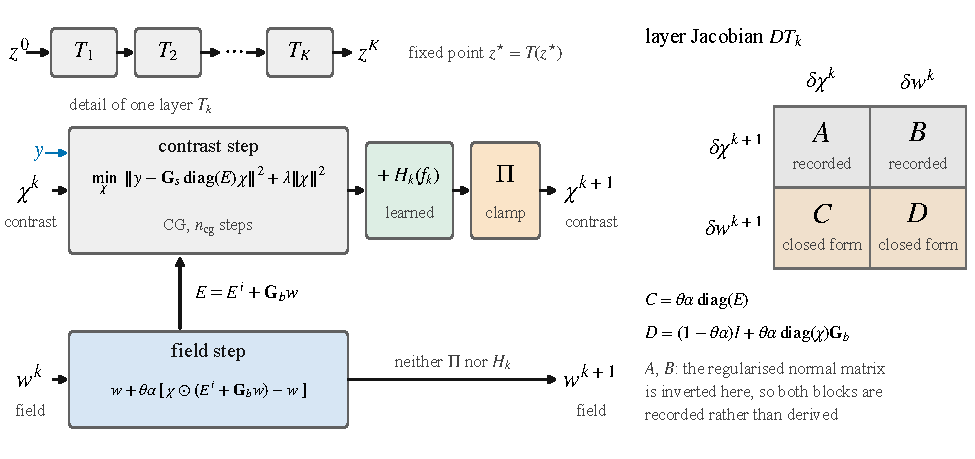
\includegraphics[width=\linewidth]{figures/fig_structure.pdf}
\caption{一个展开层及其 Jacobian。上：展开级联，其极限点满足 $z^{\star}=T(z^{\star})$。左下：单层的两个状态通道。右：$(\delta\chi,\delta w)$ 下的层 Jacobian 块图，行是离开该层的通道、列是进入它的通道。}
\label{fig:structure}
\end{figure}

\section{收敛理论}\label{sec:theory}
图~\ref{fig:structure} 固定了本节所分析的对象：一个展开层、它的两条更新路径，以及引理~\ref{lem:blocks} 精确求值的四个 Jacobian 块。

\emph{三个性质，以及其中哪些被证明了。} 下面的结果常被读作仿佛是关于“网络”的一条单一论断，因此我们在此把它们分开一次，论文其余部分保持这一区分。它们涉及不同的映射，且彼此之间没有一条能推出下一条：\emph{(C) 场子系统的收缩}在冻结对比度下是单条仿射更新在某一个通道上的性质；\emph{(B) 显式紧集的不变性}是展开轨迹的性质，且需要对比度投影；\emph{(F) 收敛性}是完整复合映射的性质，且将需要一个唯一吸引不动点。表~\ref{tab:hierarchy} 记录了假设、每个结果确立了什么、以及它明确没有确立什么。贯穿全文，$J$ 表示\emph{去掉了已学习修正}、并把投影指示在核心自变量处求值的\emph{松弛物理核}的 Jacobian，$DT_k$ 表示\emph{按实现方式}求微的第 $k$ 层 Jacobian（含截断 CG 求解与施加于复合自变量的投影）；二者只共享第二块行，此外无共同点，正如引理~\ref{lem:blocks} 所精确刻画的。

\begin{table}[htbp]
\centering
\caption{保证的层级。每一行是关于不同映射的一条论断，最后一列是未被声称的部分；前三行被证明，第四行未被证明。}
\label{tab:hierarchy}
\small
\begin{tabular}{@{}p{0.17\linewidth}p{0.24\linewidth}p{0.26\linewidth}p{0.24\linewidth}@{}}
\toprule
性质 & 对象 & 何时被确立 & 未被确立 \\
\midrule
(C) 场收缩 & $w\mapsto(1-\alpha)w+\alpha\chi\odot(E^i+\mathbf{G}_bw)$，于冻结 $\chi$ 处
& $\beta_0<1$，所有 $\alpha\in(0,1]$，速率 $1-\alpha(1-\beta_0)$（定理~\ref{thm:field}）
& 关于复合层或关于 $\chi$ 的任何事情 \\
(B) 有界展开 & 处于 $K$ 层下的完整状态 $(\chi,w)$
& 每层投影，$\beta_0<1$，$\inf_k\theta_k\alpha_k>0$（定理~\ref{thm:bounded}）
& 不动点的存在性、唯一性或吸引性 \\
非收缩性 & 单整层，$DT_k$ & $\alpha>\alpha_c$，对比度通道上任意修正（命题~\ref{prop:imposs}） & 该层在 $\alpha_c$ \emph{以下}是收缩的 \\
(F) 收敛性 & 重复复合 $T^K$
& 本文未证明；将需要 $\rho_\chi<1$，该量已被实测但未被证实
& 全局收敛、唯一不动点或无条件噪声增益 \\
\bottomrule
\end{tabular}
\end{table}

贯穿全文，$B\subset\R^n\times\C^{n\times n_{\mathrm{inc}}}$ 是由定理~\ref{thm:bounded} 提供的不变紧集；只要投影处于活动状态，它就包含物理不动点，且下面所有常数都在 $B$ 上定义。我们采用
\begin{equation}\label{eq:budgets}
\bar\epsilon := \sup_{k}\sup_{z\in B}\norm{H_k(z;y)},\qquad
\ell := \sup_k \operatorname{Lip}\big(H_k(\cdot;y)\big),
\end{equation}
以及对于容许对比度上界 $\chi_{\max}$，
\begin{equation}\label{eq:beta0}
\beta_0 \;:=\; \chi_{\max}\,\norm{\mathbf{G}_b}_2 .
\end{equation}
条件 $\beta_0<1$ \emph{不是}本文的贡献：它是 \eqref{eq:ls} 在算子范数意义下的 Neumann 级数经典的收敛条件 \cite{born_lit}，且自该领域起源以来就已知该级数只保证在阈值一侧收敛，而只能通过修改级数把它推过阈值，正如 Kleinman 与 van den Berg \cite{kleinvandenberg} 以及 Kleinman 等人 \cite{convergentborn} 所示；由它推出的、一阶近似的弱散射有效性限制同样也是经典的 \cite{slaney}。
本文的新意仅在于它作为定理~\ref{thm:field} 展开式 rollout 证书的\emph{假设}所扮演的角色，连同实测值 $\beta_0^{\mathrm{meas}}=\numv{\NumBetaMeas}>1$。这里必须区分两个工作点，且全文都保持区分：该假设对“去掉投影重新训练”的臂\emph{失效}（其对比度离开被认证盒子，$\infn{\chi}=\numv{\NumAblUncPOffFbOnChi}$），而在被认证的对比度盒 $\chi_{\max}=\numv{\chimax}$ 处同一常数 $\beta_0=\numv{\betacert}<1$ 且假设\emph{成立}（由定理~\ref{thm:field}）。本段所引用的实测值指两者中的第一个，而定理~\ref{thm:field} 的认证值指第二个；二者并不冲突。
对于非正规算子，$\sigma_{\max}$ 与 $\rho$ 不同，而正是这一差异——而非疏漏——使下面某些论断成为条件性的；在出现之处我们显式说明并报告实测量。

\subsection{为何逐层欧氏收缩是不可能的}
这一障碍从层 Jacobian 的块结构中读出，我们先把它记录如下。

\begin{Lemma}[精确块结构]\label{lem:blocks}
设 $J=\left[\begin{smallmatrix}A&B\\ C&D\end{smallmatrix}\right]$ 为\emph{松弛物理核}在
$z=(\chi,w)$ 处、按状态次序 $(\chi,\mathrm{Re}\,w,\mathrm{Im}\,w)$ 的实化 Jacobian，即
$\chi^{+}=\mathbf{1}_{\Pi}[(1-\theta\gamma)\chi+\theta\gamma\,\hat\chi^{\mathrm{LS}}(\chi,w)]$
与 $w^{+}=(1-\theta\alpha)w+\theta\alpha\,\chi\odot(E^{i}+\mathbf{G}_b w)$ 的 Jacobian，\emph{且已排除已学习修正 $H_k$}。完整层 Jacobian $DT_k$ \emph{并非} $J+DH_k$，而这一差别至关重要。如算法~\ref{alg:layer} 所示，$\Pi$ 施加于\emph{复合}自变量 $a_{\mathrm{core}}+H_k$，其中
$a_{\mathrm{core}}:=\chi+\theta(\chi^{t}-\chi)$，而 $J$ 是在仅于 $a_{\mathrm{core}}$ 处求值的投影指示下对核心求微。因此
\begin{equation}\label{eq:dTvsJ}
DT_k-J=\Big(\mathbf{1}_{\Pi}^{(a_{\mathrm{core}}+H_k)}-\mathbf{1}_{\Pi}^{(a_{\mathrm{core}})}\Big)M_{\mathrm{core}}+\mathbf{1}_{\Pi}^{(a_{\mathrm{core}}+H_k)}\frac{\partial H_k}{\partial z},
\end{equation}
其中 $M_{\mathrm{core}}:=\partial a_{\mathrm{core}}/\partial z$，$\mathbf{1}_{\Pi}^{(\cdot)}$ 为 $\Pi$ 在所陈自变量处活跃分支的对角 $0/1$ 指示。两边都是针对 $\chi$-输出块行书写的：$M_{\mathrm{core}}$ 为 $n\times(n+2nn_{\mathrm{inc}})$，每个指示为 $n\times n$ 并在左侧与之相乘，$\partial H_k/\partial z$ 为 $n\times(n+2nn_{\mathrm{inc}})$，因此乘积按此次序可乘，且三项均为 $n\times(n+2nn_{\mathrm{inc}})$；$DT_k$ 与 $J$ 的 $w$-输出行相同，因此差值对应的行恰为零。当投影不活跃时第一项（投影指示差）消失，差值退化为第二项 $\partial H_k/\partial z$，它由 $\operatorname{Lip}(H_k)$ 控制；而 $\operatorname{Lip}(H_k)$ \emph{不}控制的是第一项，即投影指示差，当 $H_k$ 把某单元推过夹紧界时可以大到 $\norm{M_{\mathrm{core}}}$。区间投影子 $\Pi_{[0,\chi_{\max}]}$ 在边界处不可微；下面的块分解使用活跃分支指示 $\mathbf{1}_{\Pi}$，即经典的右导数约定，且被认证的块 $C$ 与 $D$ 根本不触及对比度投影，因此不可微性不影响不可能性证书。对两个算子都\emph{精确}的是第二块行：场更新 $w^{+}=w+\theta(w_t-w)$ 既不被投影也不被修正，因此它向 $J$ 与 $DT_k$ 同样地贡献同一个 $C$ 与 $D$。于是，令
$E=E^i+\mathbf{G}_b w\in\C^{n_{\mathrm{inc}}\times n}$ 为 $z$ 处的总场，有
\begin{equation}\label{eq:blocks}
C \;=\; \theta\,\alpha\,\mathrm{diag}(E),\qquad
D \;=\; (1-\theta\alpha)I+\theta\alpha\,\mathrm{diag}(\chi)\,\mathbf{G}_b ,
\end{equation}
而 $A=\mathbf{1}_{\Pi}\big[(1-\theta\gamma)I+\theta\gamma\,
\partial\hat\chi^{\mathrm{LS}}/\partial\chi\big]$ 与
$B=\theta\gamma\,\partial\hat\chi^{\mathrm{LS}}/\partial w$，两者都在 $a_{\mathrm{core}}$ 处求值 $\mathbf{1}_{\Pi}$：这两个是\emph{核心}的 $\chi$-块，而非 $DT_k$ 的。因此能够迁移到 $DT_k$ 的界就是第二块行上的 $C$ 与 $D$。
\end{Lemma}
\begin{proof}
在状态次序下，$w^{+}$ 只通过对角因子
$\chi\odot(E^i+\mathbf{G}_b w)$ 依赖于 $\chi$，其对 $\chi$ 的导数为
$\mathrm{diag}(E^i+\mathbf{G}_b w)$；\eqref{eq:layer-code} 中的松弛把它乘以
$\theta\alpha$，得到 $C$。$w$-块由
$\partial w^{+}/\partial w=I+\theta\alpha(\mathrm{diag}(\chi)\mathbf{G}_b-I)$ 得到 $D$。核心的 $\chi$-块为 $\chi^{t}=(1-\gamma)\chi+\gamma\hat\chi^{\mathrm{LS}}$，而
$\hat\chi^{\mathrm{LS}}$ 如第~\ref{sec:form} 节所述只通过 $w^{+}$ 依赖于 $\chi$，由此得到
$A$ 与 $B$；投影在 $a_{\mathrm{core}}$ 处贡献 $0/1$ 因子 $\mathbf{1}_{\Pi}$，此外是非扩张的。对层\emph{按实现方式}求微，即对施加于 $a_{\mathrm{core}}+H_k$ 的投影、且 $H_k$ 自身在内部被求微，则给出 \eqref{eq:dTvsJ}。加性恒等式 $DT_k=J+DH_k$ 的两側在 $\Pi$ 不活跃或关闭时恰相吻合，这一点由非对角残差直接确认：投影关闭时为 \numv{\NumTOneRelOff}，开启时为 \numv{\NumTOneRelOn}，二者都相对于 $\norm{DT_kv}$。
\end{proof}
关于 $C$ 需要两条注记，以便下一个命题不致被错误引用。首先，\eqref{eq:blocks} 中的算子作用于\emph{空间}对比度块并产生一个\emph{按入射堆叠}的场块：它是沿单元 $r$ 对秩一映射 $\delta\chi_r\mapsto\theta\alpha E_{\cdot,r}\,\delta\chi_r$ 的直和，其中 $E_{\cdot,r}\in\C^{n_{\mathrm{inc}}}$ 是 $E$ 的第 $r$ 列。因此其奇异值为
$\theta\alpha\norm{E_{\cdot,r}}_2$，$r=1,\dots,n$，其中 $\norm{\cdot}_2$ 取\emph{沿入射轴}的范数。其次，量 $\max_r|E(r)|$（场的 $\ell_\infty$ 范数）是一个不同的对象，满足
$\max_r|E(r)|\le\max_r\norm{E_{\cdot,r}}_2\le\sqrt{n_{\mathrm{inc}}}\,\max_r|E(r)|$；在我们的离散化中二者相差因子 $\numv{\NumEInfRatio}$。下面每个范数论断都采用列范数
\begin{equation}\label{eq:Ecol}
\mathcal{E}\;:=\;\max_{r}\norm{E_{\cdot,r}}_2 ,
\end{equation}
即跨入射的逐单元最大场能量。

\begin{Proposition}[复合收缩的不可能性：阈值形式]\label{prop:imposs}
下面所有范数都是实状态 $(\chi,\operatorname{Re}w,\operatorname{Im}w)$ 上的等权欧氏范数。因此该界依赖于坐标：对场变量的一次线性缩放会重新缩放耦合块 $C$，并连同它一起重新缩放阈值 $\alpha_c=(\theta\mathcal{E})^{-1}$，所以这种不可能性是关于此度量的论断，而非架构无关的事实。该缩放并不弱化论断：它只是在另一范数下重述同一物理映射，阈值随范数移动；在每一等权选择下都存活的是如下事实：存在那些步长——即在所选度量中处于 $\alpha_c$ 之上的那些——在其上没有任何对比度通道修正能恢复一个收缩层。采用这一约定，对每一 $\alpha,\gamma\in(0,1]$ 与每一 $z\in B$，层 Jacobian 满足三个\emph{严格的}下界
\begin{equation}\label{eq:impossbound}
\sigma_{\max}(J)\;\ge\;\underbrace{\theta\alpha\,\mathcal{E}}_{\sigma_{\max}(C)}\;,
\qquad
\sigma_{\max}(J)\;\ge\;\sigma_{\max}(B)\;,\qquad
\sigma_{\max}(J)\;\ge\;\sigma_{\max}(A),
\end{equation}
其中第一个具有显式闭式，因为 $C$ 是秩一块的直和，如引理~\ref{lem:blocks} 所示。于是层映射在整个步长范围
\begin{equation}\label{eq:alphac}
\alpha>\alpha_c:=(\theta\,\mathcal{E})^{-1},
\end{equation}
上被证明为非收缩的，即那里 $\sigma_{\max}(J)>1$，且 $\alpha_c$ 随峰值场列范数 $\mathcal{E}$ 增大而减小。此外，\emph{完整}层 Jacobian 无附加假设即继承第一个界：由于第二块行由引理~\ref{lem:blocks} 为 $J$ 与 $DT_k$ 共有，一个支撑于对比度输入块的单元测试向量给出
\begin{equation}\label{eq:imposscomp}
\sigma_{\max}(DT_k)\;\ge\;\sigma_{\max}(C)=\theta\alpha\,\mathcal{E}>1
\qquad(\alpha>\alpha_c),
\end{equation}
对任意局限于对比度通道的修正 $H_k$（因此共有的 $\chi\!\to\!w$ 块 $C$ 不变）与任意 Lipschitz 常数 $\ell$ 都成立。在这一步长范围上，没有任何这样的修正能恢复 $\sigma_{\max}(DT_k)<1$：障碍作用在 $\chi\!\to\!w$ 通道，这是仅施加于对比度的修正所无法触及的。该阈值是非收缩性的一个\emph{充分}条件而非必要条件：在 $\alpha_c$ 之上，对每个可容许修正都证明了非收缩性；在其之下，\eqref{eq:impossbound} 中的下界不再超过一，问题由数值而非解析解决，如图~\ref{fig:alphac}。
\end{Proposition}
\begin{proof}
三个界都是同一个基本事实的实例：对一个支撑于单个块的测试向量，$\sigma_{\max}(J)\ge\norm{J(v,0)}$ 或 $\ge\norm{J(0,u)}$，且 $J(v,0)=(Av,Cv)$ 而 $J(0,u)=(Bu,Du)$。取 $v$ 为 $C$ 的领首右奇异向量，得 $\norm{J(v,0)}\ge\norm{Cv}=\sigma_{\max}(C)$；取 $u$ 为 $B$ 的领首右奇异向量，得 $\norm{J(0,u)}\ge\sigma_{\max}(B)$；取 $v$ 为 $A$ 的领首右奇异向量，由同一恒等式得 $\sigma_{\max}(J)\ge\sigma_{\max}(A)$。第一个界的闭式：$C$ 是沿单元对秩一映射 $\delta\chi_r\mapsto\theta\alpha E_{\cdot,r}\delta\chi_r$ 的直和（引理~\ref{lem:blocks}），其奇异值为 $\theta\alpha\norm{E_{\cdot,r}}_2$；最大的是 $\theta\alpha\mathcal{E}$，在 $v=e_{r^\star}$、$r^\star=\arg\max_r\norm{E_{\cdot,r}}_2$ 处取到。方向很重要：一个\emph{任意}的单位 $v$ 只给出
$\norm{Cv}\ge\theta\alpha\min_r\norm{E_{\cdot,r}}_2\norm{v}$，而会出错的正是那种 $\ell_\infty$ 版本 $\max_r|E(r)|$，它由 \eqref{eq:Ecol} 下讨论的因子给出。式~\eqref{eq:alphac} 重整 $\theta\alpha\mathcal{E}>1$。最后，由引理~\ref{lem:blocks}，$C$ 同时是 $DT_k$ 与 $J$ 的一个块（对任何不改变 $\chi\!\to\!w$ 块的修正而言），因此同样的测试向量论证给出 \eqref{eq:imposscomp}，无需援引 \eqref{eq:dTvsJ}，也无需对这样的 $H_k$ 作任何假设；作用于 $w$-通道的修正原则上可以改变 $C$，不在该论断覆盖之内。
\end{proof}

\begin{Remark}[Weyl 扰动路径]\label{rem:weyl}
应用于加性分解 $DT_k=J+DH_k$ 的 Weyl 不等式会给出
$\sigma_{\max}(DT_k)\ge\sigma_{\max}(J)-\operatorname{Lip}(H_k)$。而这一分解正是 \eqref{eq:dTvsJ} 所排除的，因此该不等式在此不适用，我们也不援引它。
尽管如此，比较中的三个量仍被报告，因为它们来自\emph{同一个}驱动与\emph{同一个}状态，即 \texttt{gain\_decomp.json} 的约束臂，处于已学习步长与已实现的 $n_{\mathrm{cg}}$ 下，从而使比较从一开始就是良定的：
$\sigma_{\max}(J)=\numv{\NumGdPhysSigma}$，
$\operatorname{Lip}(H_k)=\numv{\NumLipHCons}$，因此 Weyl 下界
$\sigma_{\max}(J)-\operatorname{Lip}(H_k)=\numv{\NumWeylRhs}$，而实测逐层复合为 $\numv{\NumSigCompLayerCons}$。用修正后的算子，这两个数满足该界而非违反它：$\numv{\NumWeylRhs}\le\numv{\NumSigCompLayerCons}$，因此 Weyl 不等式被满足，无从读出数值矛盾。扰动路径仍不能推出 \eqref{eq:imposscomp} 的原因因此是\emph{结构性的}而非数值的：\eqref{eq:dTvsJ} 排除了加性分解 $DT_k=J+DH_k$，因为投影作用于复合自变量，所以 $DT_k$ 的耦合块不是 $J$ 的耦合块再加一个修正的块；这与上面的量级无关地成立。因此命题~\ref{prop:imposs} 的块论证不是扰动界的更强变体，而是唯一适用的那一个：它根本不需要分解 $DT_k$，因为耦合块 $C$ 为 $J$ 与 $DT_k$ 共有。保留这些数字，是为了让走到扰动路径的读者能验证 Weyl 下界被满足，并看到为何它所需的分解在结构上仍不可用。一个直接的数值检查以双精度零相对误差复现了块结构以及共有第二行的精确性，并确认了投影开/关的控制。
\end{Remark}

有四点固定了解读。\emph{(a) 裕度依赖于 $\alpha$。} 被认证的裕度为 $\kappa(\alpha)=\theta\alpha\mathcal{E}-1>0$（在 $\alpha>\alpha_c$ 上），且随 $\alpha\downarrow\alpha_c$ 而消失；由 \eqref{eq:impossbound} 推不出任何与 $\alpha$ 无关的裕度，我们也未作此类声称。块结构直接支持的唯一的 $\alpha$-一致下界是较弱的包络
$\sigma_{\max}(J(\alpha))\ge1-\theta\alpha(1+\beta_0)$，它来自
$\sigma_{\max}(J)\ge\sigma_{\min}(D)\ge1-\theta\alpha(1+\beta_0)$，其中
$\sigma_{\min}(D)$ 是直接块 $D$ 的最小奇异值。\emph{(b) 该界按工作点陈述并数值求值。} $\mathcal{E}$、$\sigma_{\max}(A)$ 与 $\sigma_{\max}(B)$ 都依赖于 $z$；因此我们报告它们在\emph{实际达到}的工作点处的值，列于表~\ref{tab:cert}，而非 $z$-无关常数，且我们显式陈述 $\alpha$ 依赖而非把它塞进单一数字。阈值 $\alpha_c=(\theta\mathcal{E})^{-1}$ 进一步继承了场归一化：当入射场缩放至单位峰值，则 $\mathcal{E}=\max_r\|E_{\cdot,r}\|_2$ 随照明数按 $\sqrt{n_{\mathrm{inc}}}$ 缩放，因此跨配置的 $\alpha_c$ 比较必须连同其 $n_{\mathrm{inc}}$ 与归一化一起读，而非作为纯架构论断。\emph{(c) 在 $\alpha_c$ 以下该界无法下结论，因此我们去测量。} 对 $\alpha\le\alpha_c$ 由 \eqref{eq:impossbound} 推不出任何东西；图~\ref{fig:alphac} 与表~\ref{tab:cert} 在以网格 $\alpha\in[0.05,1]$ 报告实测的 $\sigma_{\max}(J(\alpha))$，并标出每一点落在 $\alpha_c$ 的哪一侧。\emph{(d) 障碍是双线性的，而非数据失配非线性的产物。} 把对比度步中的自洽场替换为固定入射场 $E^i$（即 Born 变体，对其由引理~\ref{lem:blocks} 有 $B\equiv0$）不动 $C$（$\sigma_{\max}(C)=\numv{\NumBornSigmaC}$，与忠实值 $\numv{\NumSigCLower}$ 相同），且实测复合仍高于一（$\numv{\NumBornSigmaFull}$，表~\ref{tab:cert}）。该变体还有两个解析透明的块：由于其对比度步不再依赖于场状态，$\sigma_{\max}(B)\equiv0$ 且 $\sigma_{\max}(A)=1-\gamma$ 精确成立（在工作点处投影不活跃时）。仪器把二者都复现到机器精度（$\numv{\NumBornSigmaA}$ 与 $\numv{\NumBornSigmaB}$），这是第三个精确自检，独立于 $C$ 的闭式。因此非收缩性是由\emph{场}步中的双线性耦合 $\chi\odot E$ 产生的，无法通过把数据失配线性化来消除。

命题~\ref{prop:imposs} 是关于\emph{架构}的论断，而非关于训练的：在 $\alpha>\alpha_c$ 上，展开文献全程使用的自然充分条件——一个欧氏收缩层映射——对忠实的 Born/对比度源网络不可用，对任何局限于对比度通道的修正（在命题所声明的坐标与通道限定下）都不可用。认证因此必须是\emph{分层}的。

\subsection{可被认证的：场子系统、有界性、保真度}
图~\ref{fig:regime} 把本节的两个区域定位在同一平面上；它们并不互斥，且重叠正是本文的实质而非其缺口。在合成工作点处同时有 $\beta_0=\numv{\betacert}<1$，因此\emph{场子系统}由定理~\ref{thm:field} 收缩，且 $\alpha>\alpha_c=\numv{\NumAlphaC}$，因此\emph{复合层}由命题~\ref{prop:imposs} 被证明为非收缩的。

\begin{figure}[htbp]
\centering
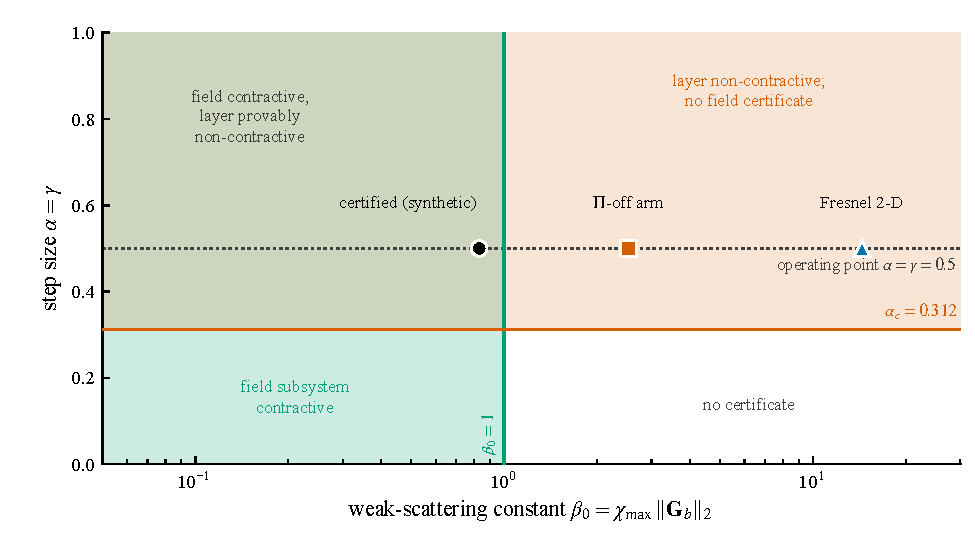
\includegraphics[width=\linewidth]{figures/fig_regime.pdf}
\caption{$(\beta_0,\alpha)$ 平面中的区域。在 $\beta_0=1$ 左侧场子系统被证明收缩，在 $\alpha=\alpha_c$ 上方复合层被证明非收缩，其重叠即被认证的配置。三个标记分别是合成盒、去掉投影重新训练的臂，以及 Fresnel 几何。}
\label{fig:regime}
\end{figure}

\begin{Theorem}[先验场子系统收缩]\label{thm:field}
固定任意容许对比度，满足 $\infn{\chi}\le\chi_{\max}$。则对每一 $\alpha\in(0,1]$，阻尼场步 \eqref{eq:fieldstep} 在 $w$ 上是仿射的，Jacobian 为
$J_w=(1-\alpha)I+\alpha\,\mathrm{diag}(\chi)\mathbf{G}_b$，且
\begin{equation}\label{eq:fieldcontract}
\norm{J_w}_2 \;\le\; 1-\alpha\,(1-\beta_0),\qquad
\beta_0=\chi_{\max}\norm{\mathbf{G}_b}_2 .
\end{equation}
特别地，若 $\beta_0<1$，则场子系统对\emph{每个}步长在对比度源上都是收缩的，速率为 $1-\alpha(1-\beta_0)$。
\end{Theorem}
\begin{proof}
$\norm{\mathrm{diag}(\chi)\mathbf{G}_b}_2\le\infn{\chi}\norm{\mathbf{G}_b}_2\le\beta_0$，故
$\norm{J_w}_2\le(1-\alpha)+\alpha\beta_0$。
\end{proof}
在我们的离散化中 $\norm{\mathbf{G}_b}_2=\numv{\gbnorm}$、$\chi_{\max}=\numv{\chimax}$，给出 $\beta_0=\numv{\betacert}<1$：弱散射机制在\emph{任何训练之前}即可被认证，且它是理论中唯一属于物理而非已学习参数的成分。

\begin{Theorem}[展开轨迹的被认证有界性]\label{thm:bounded}
假设 (i) 物理先验投影 $\chi\leftarrow\Pi_{[0,\chi_{\max}]}(\chi)$ 在每层之后施加；(ii) $\beta_0<1$；以及 (iii) 初始对比度满足 $\infn{\chi^{0}}\le\chi_{\max}$，且 $\inf_k\theta_k\alpha_k>0$，使得逐层速率 $1-\theta_k\alpha_k(1-\beta_0)$ 容许一个严格小于 $1$ 的一致上界。则对每一 $K\ge0$、每一训练参数集以及每一阻尼/松弛序列 $\{(\alpha_k,\gamma_k,\theta_k)\}\subset(0,1]^{3}$，
\begin{equation}\label{eq:box}
\begin{aligned}
&\infn{\chi^{K}}\le\chi_{\max},\qquad
\norm{w^{K}}\le(\gamma_w^{+})^{K}\norm{w^{0}}
+\frac{\bar\theta\bar\alpha\,\chi_{\max}\norm{E^i}}{1-\gamma_w^{+}},\\
&\gamma_w^{+}=1-\underline{\theta\alpha}\,(1-\beta_0),\qquad
\underline{\theta\alpha}:=\inf_k\theta_k\alpha_k>0,\qquad
\bar\theta\bar\alpha:=\sup_k\theta_k\alpha_k\le1,
\end{aligned}
\end{equation}
其中 $\gamma_w^{+}$ 是\emph{最大}逐层速率，
$\gamma_w^{+}=\sup_k\big(1-\theta_k\alpha_k(1-\beta_0)\big)$；因为对每一 $k$ 有 $\gamma_w^{+}\ge1-\theta_k\alpha_k(1-\beta_0)$，递推被一个公比为 $\gamma_w^{+}<1$ 的几何和从上方界定。因此轨迹从不离开显式紧集
$B=\{\infn{\chi}\le\chi_{\max}\}\times\{\norm{w}\le
\max\big(\norm{w^{0}},\;\chi_{\max}\norm{E^i}/(1-\gamma_w^{+})\big)\}$，
与深度无关；若 $\norm{w^{0}}\le\chi_{\max}\norm{E^i}/(1-\gamma_w^{+})$，则盒为
$B=\{\infn{\chi}\le\chi_{\max},\ \norm{w}\le\chi_{\max}\norm{E^i}/(1-\gamma_w^{+})\}$，且 $(\gamma_w^{+})^{K}$ 项为多余。
\end{Theorem}
\begin{proof}
$\chi$-界是 $\Pi$ 的定义。对场变量，取
$w^{k+1}=w^{k}+\theta_k\alpha_k\big(\chi^{k}\odot(E^i+\mathbf{G}_b w^{k})-w^{k}\big)$ 的范数，并用
$\norm{\mathrm{diag}(\chi)\mathbf{G}_b}_2\le\beta_0$ 得
$\norm{w^{k+1}}\le\big[1-\theta_k\alpha_k(1-\beta_0)\big]\norm{w^{k}}
+\theta_k\alpha_k\chi_{\max}\norm{E^i}$，这是一个仿射递推，其逐层速率 $1-\theta_k\alpha_k(1-\beta_0)$ 被其上确界
$\gamma_w^{+}=1-\underline{\theta\alpha}(1-\beta_0)$（其中 $\underline{\theta\alpha}=\inf_k\theta_k\alpha_k>0$）从上方界定，其强迫项被 $\bar\theta\bar\alpha\chi_{\max}\norm{E^i}$ 从上方界定；迭代即得 \eqref{eq:box}，瞬态项仅当 $\norm{w^0}$ 起始于静止半径之外时才需要。
\end{proof}
这三个假设在工作点处被 discharged 而非假设。(i) 是每一个被认证臂都设置的结构性标志；(ii) 是被认证的 $\beta_0=\numv{\betacert}$；(iii) 由参数化的构造成立，因为步长为 $\alpha_k=a_{\max}\sigma(a_k)$、$\gamma_k=g_{\max}\sigma(g_k)$，其中 $\sigma$ 为 logistic 函数且 $\theta_k\equiv1$，因此每个值对每个层、每次训练迭代都落在 $(0,a_{\max}]$ 内，且有限个层上的下确界是一个严格为正的极小值。非结构性的是该极小值的\emph{大小}：它是被学习的，因此训练设定了盒的宽度而非其存在性。
两点值得强调。首先，假设 (i) 是 $\chi$ 上界的\emph{唯一}来源：一个不加 $\Pi$ 训练的网络仍可能碰巧保持有界，但相应的界必须被\emph{实测}，而在我们的实验中实测值 $\infn{\chi}=\numv{\NumMeasChiNoProj}$ 给出
$\beta_0^{\mathrm{meas}}=\numv{\NumBetaMeas}>1$，因此定理的假设失效，没有任何先验论断存活。其次，修正 $H_k$ 根本不进入盒：它在 $\Pi$ 之前作用于对比度通道，而 $\Pi$ 把结果对任何修正都夹紧到 $[0,\chi_{\max}]$，且场递推中不含 $H_k$。有界修正的作用在别处：推论~\ref{cor:fidelity} 的保真度半径 $\bar\epsilon/(1-\rho_\chi)$ 只有当漂移 $\norm{\hat G-F}_\infty$ 有限时才有限，而后者由振幅预算、更根本地由约束主干输入提供，连同注记~\ref{rem:featscale}。

\begin{Corollary}[用于无限深度外推的条件漂移界]\label{cor:fidelity}
定义\emph{物理对比度映射}及其不动点
\begin{equation}\label{eq:chistar}
F(\chi):=\Pi\big(\hat\chi^{\mathrm{LS}}\big(E(\chi);y\big)\big),\qquad
\chi^{\star}:=F(\chi^{\star}),
\end{equation}
其中 $E(\chi)=E^i+\mathbf{G}_b w(\chi)$，$w(\chi)$ 对给定 $\chi$ 解离散场方程
$w=\chi\odot(E^i+\mathbf{G}_b w)$；于是 $\chi^{\star}$ 恰为命题~\ref{prop:fixpoint} 物理不动点 $z^{\star}$ 的 $\chi$-分量。对 $P$ 个重复训练层副本的循环复合 $T^{P}:=T\circ\cdots\circ T$，定义\emph{修正对比度映射} $\hat G(\chi):=\pi_\chi\big(T^{P}(\chi,w(\chi))\big)$，使用与 $F$ 相同的精确场解 $w(\chi)$；因此 $\hat G$ 是一个\emph{代理}：它在每个周期后把场重置为精确解，而真实展开轨迹保留阻尼场更新，所以 $\hat G$ 的不动点不必与重复层 $T^P$ 的不动点重合，且下面的 (c) 只界定到 $\chi^\star$ 的距离，且只针对这一代理。假设
(a) $\hat G$ 在 $B$ 中有一个不动点 $\hat\chi$；(b) $F$ 在 $B$ 上全局 Lipschitz，常数 $\rho_\chi<1$，即 $\sup_{\chi\in B}\norm{DF(\chi)}_2<1$，它严格强于逐点谱半径条件；且 (c) $\sup_{\chi\in B}\norm{\hat G(\chi)-F(\chi)}\le\delta_{\mathrm{GF}}$，其中 $\delta_{\mathrm{GF}}$ 是修正映射相对物理映射的\emph{漂移}，是与 \eqref{eq:budgets} 的主干振幅预算 $\bar\epsilon$ 不同的一个\emph{独立}常数：二者一般不相等。在 $H\equiv0$ 时漂移不为零，而是一次精确对比度更新与 $P$ 个阻尼层之间的松弛偏置，且它也不受 $\bar\epsilon$ 控制。
则
\begin{equation}\label{eq:fidelity}
\norm{\hat\chi-\chi^{\star}}\;\le\;\frac{\delta_{\mathrm{GF}}}{1-\rho_\chi}.
\end{equation}
若另有 (d) $\hat G$ 在 $B$ 上为 $\hat\rho$-Lipschitz 且 $\hat\rho<1$，则 $\hat\chi$ 是 $\hat G$ 在 $B$ 中的唯一不动点，且迭代 $\hat G$ 在 $O\big(\log(1/\delta)/\log(1/\hat\rho)\big)$ 层内达到精度 $\delta$。
\end{Corollary}
\begin{proof}
$\norm{\hat\chi-\chi^{\star}}=\norm{\hat G(\hat\chi)-F(\chi^{\star})}
\le\norm{\hat G(\hat\chi)-F(\hat\chi)}+\norm{F(\hat\chi)-F(\chi^{\star})}
\le\delta_{\mathrm{GF}}+\rho_\chi\norm{\hat\chi-\chi^{\star}}$，解出范数即得 \eqref{eq:fidelity}；只用到在 $\hat\chi$ 处求值的 (b) 与 (c)，因此这一部分不需要 $\hat G$ 的收缩性。唯一性与几何速率是 Banach 不动点定理在 (d) 下对 $\hat G$ 的应用。仅假设 (c) 并\emph{不}使 $\hat G$ 成为收缩：它约束距离 $\norm{\hat G-F}_\infty$ 而对 $\hat G$ 的 Lipschitz 常数只字未提，且一个收缩的“有界距离”扰动可以有任意大的 Lipschitz 常数——一个高度为 $\bar\epsilon$、宽度任意小的隆起即满足 (c) 而其 Lipschitz 常数无界增长。因此唯一性与 $O(\log(1/\delta))$ 速率依赖于独立的假设 (d)，而 (d) 我们在此并不声称成立；在我们的实测中连更弱的 (b) 也不成立。
\end{proof}
该假设落在定义 $\chi^{\star}$ 的映射 $F$ 上，而非落在修正映射 $\hat G$ 上；二者仅在 $H\equiv0$ 处重合。由此引出两个警示，且它们\emph{不是}我们在此能够 discharged 的假设。

首先，$\rho_\chi<1$ 是一个假设而非定理：先验可用的唯一收缩常数是 $\beta_0<1$，它界定的是\emph{场}子系统 \eqref{eq:fieldcontract} 而对 $F$ 只字未提。事实上
$\partial F/\partial\chi=(\partial\hat\chi^{\mathrm{LS}}/\partial E)(\partial E/\partial\chi)$，其中
$\norm{\partial E/\partial\chi}_2\le\norm{\mathbf{G}_b}_2/(1-\beta_0)=\numv{\NumdEdChi}$，而
$\partial\hat\chi^{\mathrm{LS}}/\partial E$ 被（正则化）法矩阵的逆放大，其最小特征值为 $\numv{\NumLamMin}$；因此在半径中用 $\beta_0$ 替代 $\rho_\chi$ 是不合理的，且 $\bar\epsilon/(1-\beta_0)$ 绝不能被引为“先验漂移半径”。对 $F$ 与 $\hat G$ 我们都报告两个数，即 $\chi\!\to\!\chi$ 块的 $\sigma_{\max}$ 与整个 $\chi$-行 $[A\,B]$ 的范数（后者是 $\chi$-映射的 Lipschitz 常数，前者只是它的一个下界），如表~\ref{tab:cert} 所示。这些数\emph{并非}全部落在某一边：在约束臂中每一对都低于一（对 $\hat G$ 为 $\numv{\NumRhoChiCons}$ 与 $\numv{\NumChiLipRowCons}$；对 $F$ 为 $\numv{\NumChiFBlockCons}$ 与 $\numv{\NumChiLipRowFCons}$），因此那里没有任何实测量否定 $\rho_\chi<1$，而在无约束臂中 $\hat G$ 的行范数达到 $\numv{\NumChiLipRowUnc}$ 并否定了它。两个臂也都未被\emph{证实}：块值是一个下界，行范数对层映射是精确的，而缩并的 $\chi$-映射导数是 Schur 补，其范数二者都不界定。因此我们逐臂报告实测值，而不对几何假设作一般性失败的声称。因此理论的被认证内容是定理~\ref{thm:bounded} 的有界性加上定理~\ref{thm:field} 的场子系统速率；
推论~\ref{cor:fidelity} \emph{不}提供任何有限的先验半径，报告其下的实测 $\rho_\chi$ 是我们采用的记账方式。

其次，推论~\ref{cor:fidelity} 的条件性是对多次散射建模的直接代价。在 Born（单散射）线性化中，对比度步所用的场是固定的 $E^i$，因此 $\partial\hat\chi^{\mathrm{LS}}/\partial\chi=0$，$F$ 为常数映射，$\rho_\chi=0$，且 \eqref{eq:fidelity} 成为无条件半径 $\bar\epsilon$。恰恰是 $E$ 与 $\chi$ 的自洽性——使该方法对强散射体有效——使得该半径成为条件性的。

\begin{Proposition}[精确的有限深度噪声刻画]\label{prop:noise}
令 $L_k:=\operatorname{Lip}\big(T_k(\cdot;y)\big)$ 与
$\Lambda_k:=\sup_{z\in B}\norm{T_k(z;y+\Delta y)-T_k(z;y)}/\norm{\Delta y}$。则对每一 $K\ge1$ 与每一有界 $\Delta y$，
\begin{equation}\label{eq:noiseexact}
\norm{z^{K}(y+\Delta y)-z^{K}(y)}
\;\le\;\Big[\sum_{k=0}^{K-1}\Lambda_k\!\!\prod_{j=k+1}^{K-1}\!\!L_j\Big]\norm{\Delta y}.
\end{equation}
\end{Proposition}
\begin{proof}
令 $z^{k},\tilde z^{k}$ 为干净与受扰轨迹。由于 $T_k(\cdot;y)$ 与 $T_k(\cdot;y+\Delta y)$ 共享一个基点，
$\norm{\tilde z^{k+1}-z^{k+1}}
\le L_k\norm{\tilde z^{k}-z^{k}}+\Lambda_k\norm{\Delta y}$。从 $\tilde z^{0}=z^{0}$ 起迭代这一仿射递推并收集几何乘积即得 \eqref{eq:noiseexact}。
\end{proof}
式~\eqref{eq:noiseexact} 是精确的，不作任何收缩假设。在周期为 $P$ 的循环调度下，每周期放大为 $\Pi_{j=1}^{P}L_j$，因此当 $\Pi_{j=1}^{P}L_j<1$ 时噪声增益在深度上一致有界；在等式 $\Pi_{j=1}^{P}L_j=1$ 处，每周期注入 $\sum_{j=1}^{P}\Lambda_j$ 随周期数线性累积，因此若无额外衰减假设，等式本身不足以给出一致界。这是尖锐的论断；熟知的闭式只是它的一个特例，我们如此陈述之。邻近工作研究了展开前向—后向对数据扰动的稳定性 \cite{devalle2023}；我们的界针对对比度源复合层，是精确的而非微扰的，且不需要收缩假设。

\begin{Corollary}[几何界]\label{cor:noisegeo}
若另有对所有 $j$ 有 $L_j\le\rho<1$，则
\eqref{eq:noiseexact} $\le\Lambda(1-\rho^{K})/(1-\rho)\norm{\Delta y}
\le\Lambda\norm{\Delta y}/(1-\rho)$。
\end{Corollary}
\begin{proof}
\eqref{eq:noiseexact} 中每个乘积至多为 $\rho^{K-k}$；几何和随之而来。
\end{proof}
这一界是\emph{条件性的}，且在我们的设定中其假设被我们自己的实测否定：$L_j=\sigma_{\max}(J_j)$ 正是命题~\ref{prop:imposs} 证明对 $\alpha>\alpha_c$ 超过一的量，实测值
$\sigma_{\max}(J)=\numv{\NumPhysSigma}$（在 $\alpha=\gamma=\tfrac12$ 处），且 $L\in[\numv{\NumSigMin},\numv{\NumSigMax}]$（在 $\numv{\NumAlphaSweepN}$ 个离散步长、覆盖 $\alpha=\gamma\in[0.05,1]$ 的收敛定步长网格上），\emph{每一点}都是非收缩的，不止表~\ref{tab:cert} 中 $\alpha_c$ 之上的那些；在已学习步长处，$K{=}8$ 循环复合为 $\numv{\NumSigCompCons}$。因此我们并不把 $\Lambda/(1-\rho)$ 当作关于此架构的结果呈现；它仅被陈述以暴露其假设，而该假设被本应被引以支持它的同一批实验所反驳。起作用的论断是命题~\ref{prop:noise}。

\begin{Corollary}[用于非正规层的谱半径形式]\label{cor:noisenormal}
假设层 Jacobian 在 $B$ 上一致有界：对每一 $z\in B$ 与每一 $m\le K$，
$\norm{DT(z)^{m}}\le\kappa\rho^{m}$，其中 $\rho=\sup_{z\in B}\rho(DT(z))<1$ 且
$\kappa=\sup_{z\in B}\kappa_2(V(z))$。则特别地，对所有 $z\in B$ 有 $\norm{DT(z)}\le\kappa\rho$，因此复合 $T_{K-1}\circ\cdots\circ T_{k+1}$（沿轨迹的状态相关 Jacobian 之积）被 $(\kappa\rho)^{K-1-k}$ 界定，且只要 $\kappa\rho<1$，\eqref{eq:noiseexact} 至多为
$\Lambda\norm{\Delta y}\,(1-(\kappa\rho)^{K})/(1-\kappa\rho)$。
\end{Corollary}
\begin{proof}
由链式法则，复合 Jacobian 为 $DT(z_{K-1})\cdots DT(z_{k+1})$，是\emph{不同}状态相关矩阵的乘积，而非单一矩阵幂；等式 $\norm{J_{K-1}\cdots J_{k+1}}=\norm{J^{K-1-k}}$ 只在不动点处成立，那里所有因子重合。取 $m=1$ 的假设给出对每一 $z\in B$ 有 $\norm{DT(z)}\le\kappa\rho$，因此乘积对 $B$ 中每一轨迹被 $(\kappa\rho)^{K-1-k}$ 界定；对 \eqref{eq:noiseexact} 的 $K$ 项求和即得所述因子。由于 $\kappa=\sup_{z\in B}\kappa_2(V(z))$ 不被当前实测界定（只有注记~\ref{rem:mj} 的 $M_J$ 下界可得），且 $\rho<1$ 本身不能控制非正规因子的乘积，该推论\emph{不能}由当前数据给出有限噪声增益；它仅被陈述以暴露其假设。
\end{proof}
\begin{Remark}[瞬态因子]\label{rem:mj}
瞬态 $M_J:=\sup_{1\le m\le K}\norm{J^{m}}$ 是实践者想要用来替代 Lipschitz 常数的放大因子，且我们在下面测量它；然而这一替代是\emph{无效的}。由 $\rho^{m}\le\norm{J^{m}}\le\kappa_2(V)\rho^{m}$ 得 $M_J\le\kappa_2(V)$，因此 $M_J$ 是几何和所需因子的一个\emph{下}界，而 $(1-\rho^{K})/(1-\rho)$ 是附在 $\kappa_2(V)$ 上而非附在 $M_J$ 上。把二者相乘——即形如 $\Lambda\norm{\Delta y}M_J(1-\rho^{K})/(1-\rho)$ 的界会做的——会\emph{低估}真实放大，且一般不存在这样的乘积界。它已对正规 $J=0.5I$、$K=3$ 失效，那里 \eqref{eq:noiseexact} 的精确因子 $\sum_{k=0}^{K-1}\prod_{j=k+1}^{K-1}L_j$ 为 $1.75$，而 $M_J(1-\rho^{K})/(1-\rho)=0.875$；当 $J$ 不可对角化时它彻底失效，例如幂零 $J=\bigl[\begin{smallmatrix}0&10\\0&0\end{smallmatrix}\bigr]$ 与 $K=3$，那里精确因子为 $10^2+10+1=111$（$\sigma_{\max}(J)=10$），而 $\rho=0$、$\kappa_2(V)=\infty$。由 $M_J$ 可得的最粗糙界是计数项数的 $\sum_{m\le K}\norm{J^{m}}\le K M_J$；这不是唯一的一个（例如 $\sum_{k<K}\Lambda_k\norm{J^{K-1-k}}\le\Lambda_{K-1}+M_J\sum_{k<K-1}\Lambda_k$ 也只用 $M_J$），我们不强称比“所有这些界都以相同方式粗糙”更强。简言之，$M_J$ 与 $\kappa_2(V)$ 只对于正规算子才重合，而那恰恰就是谱半径\emph{是}一个 Lipschitz 常数的情形。我们报告 $M_J$ 是因为它可被重算，且它相对 $\rho$ 的比值度量了非正规性，而非因为它界定噪声增益。
\end{Remark}
推论~\ref{cor:noisegeo} 与~\ref{cor:noisenormal} 恰好相差因子 $\kappa_2(V)$：把 Lipschitz 常数替换为谱半径只对正规算子合法，而层映射在此是\emph{绝非正规的}。那一代价的代价是可测的，且我们测量了它的成分：对 $K{=}8$ 循环复合，$M_J=\numv{\NumMJCons}$（$\kappa_2(V)$ 的下界，注记~\ref{rem:mj}），对照 $\rho=\numv{\NumRhoComp}$ 与 $\sigma_{\max}=\numv{\NumSigCompCons}$，给出表~\ref{tab:cert} 中一个非正规性缺口 $\sigma_{\max}/\rho=\numv{\NumGapRatio}$。这三者属于同一个算子，即 $K{=}8$ 展开轨迹的复合 Jacobian，因此一并报告；固定 $\alpha=\gamma=\tfrac12$ 处的逐层值 $\numv{\NumSigCompLayerCons}$ 是一个不同的算子，单列。这是对“基于谱半径的界会低估瞬态多少”的定量度量。$M_J$ 的值依赖于截断所取的视界：在完整视界 $m\in\{1,2,4,8\}$ 上，同一复合在 $m=\numv{\NumMJFullArgmaxM}$（约束）处达到 $\numv{\NumMJFullCons}$，在 $m=\numv{\NumMJFullArgmaxMUnc}$（无约束）处达到 $\numv{\NumMJFullUnc}$，因此深度-2 截断并非良性简化，我们两者都报告。

\begin{table}[htbp]
\centering
\caption{每个噪声分析量的用途，以及本文关于它所确立的内容。只有第一行是一个界可用的成分；第二行是诊断；最后三行是本文未确立的假设，其中之一被实测否定。}
\label{tab:noisestatus}
\small
\begin{tabular}{@{}p{0.10\linewidth}p{0.36\linewidth}p{0.44\linewidth}@{}}
\toprule
量 & 角色 & 在本文中的状态 \\
\midrule
$\Lambda$ & 单层对数据扰动的敏感度 & 由 \eqref{eq:Lambda} 从 Tikhonov 下界与振幅预算显式界定，并已实测（$\numv{\NumLambdaMeas}$ 对 $\numv{\NumLambdaBound}$） \\
$M_J$ & 视界上的瞬态放大 $\sup_{m\le K}\norm{J^{m}}$ & 可计算（$\numv{\NumMJCons}$ 于 $K{=}8$）；是 $\kappa_2(V)$ 的\emph{下}界，而非其替代 \\
$\kappa_2(V)$ & 几何形式的非正规性因子 & 无一致上界可用；需要它的推论因此给不出有限增益 \\
$\rho<1$ & 几何界的假设 & 被实测否定：在步长网格每一点 $\sigma_{\max}>1$ \\
$\rho_\chi<1$ & 保真度半径 $\delta_{\mathrm{GF}}/(1-\rho_\chi)$ 的假设 & 既未被证实也未被否定：块值低于一（$\numv{\NumRhoChiCons}$）但它只是 Lipschitz 常数的一个下界，其行范数估计为 $\numv{\NumChiLipRowCons}$ \\
\bottomrule
\end{tabular}
\end{table}
表~\ref{tab:noisestatus} 是噪声分析所处位置的诚实总结：它提供一个\emph{条件性}误差刻画框架与一个可精确计算的深度-$K$ 因子，而非一个被认证的噪声增益，且下文没有任何地方把它当作后者呈现。

最后，$\Lambda$ 本身可被显式界定而非断言。一层通过两个通道依赖数据：正则化最小二乘对比度步
$\hat\chi^{\mathrm{LS}}=A(E)^{-1}b(E,y)$，其中
$\partial b/\partial y=\mathrm{diag}(\bar E)\mathbf{G}_s^{H}$，因而
$\norm{\partial\hat\chi^{\mathrm{LS}}/\partial y}_2
\le\max_r|E(r)|\,\norm{\mathbf{G}_s}_2/\lambda_{\min}(A)$——这里 $\ell_\infty$ 场范数是正确的，因为 $b$ 在 $y$ 上以系数 $\mathrm{diag}(\bar E)$ 线性；以及已学习修正，它通过伴随残差 $\mathbf{G}_s^{H}(\mathbf{G}_s w^{+}-y)$ 看到 $y$，其中 $\norm{\partial(\cdot)/\partial y}_2=\norm{\mathbf{G}_s}_2$，被残差通道的特征尺度与谱裁剪所衰减。合并得
\begin{equation}\label{eq:Lambda}
\Lambda\;\le\;\norm{\mathbf{G}_s}_2
\Big[\frac{\theta\gamma\max_r|E|}{\lambda_{\min}(A)}
\;+\;\frac{\bar\epsilon}{s_{\mathrm{res}}}\prod_i\norm{W_i}_2\Big],
\end{equation}
即 $\chi$-步的敏感度由实现所加的 Tikhonov 下界
$\lambda_{\min}(A)\ge c_{\mathrm{cg}}\min_j\sum_i|E_{ij}|^{2}\norm{\mathbf{G}_s(\cdot,j)}_2^{2}$ 控制，修正通道由振幅预算控制。直接实测得 $\Lambda=\numv{\NumLambdaMeas}$，对照对比度通道界 $\numv{\NumLambdaBound}$，其中 $\lambda_{\min}(A)=\numv{\NumLamMin}$、$s_{\mathrm{res}}=\numv{\NumScaleRes}$（表~\ref{tab:cert}）；在训练权重处修正项可忽略。式 \eqref{eq:Lambda} 取代了我们先前“$\Lambda$ 由构造有界”的断言：构造就是 \eqref{eq:Lambda}，且它只与 Tikhonov 下界一样好，因此 $\lambda_{\mathrm{rel}}$ 绝不能被驱动到零。

\begin{Proposition}[深度—精度—稳定性权衡]\label{prop:tri}
固定一个修正架构，令 $\mathcal{H}(\bar\epsilon,\ell)$ 为可容许修正的类，假设它是嵌套的：$\bar\epsilon_1\le\bar\epsilon_2$ 且 $\ell_1\le\ell_2$ 蕴含
$\mathcal{H}(\bar\epsilon_1,\ell_1)\subseteq\mathcal{H}(\bar\epsilon_2,\ell_2)$。则
(i) \emph{[深度]} 在推论~\ref{cor:fidelity} 的假设 (a)--(d) 下，$\hat G$ 的 $K$ 步迭代满足 $\norm{\hat G^{K}(\chi^{0})-\chi^{\star}}\le\hat\rho^{K}\norm{\chi^{0}-\chi^{\star}}
+\delta_{\mathrm{GF}}(1+\hat\rho^{K})/(1-\rho_\chi)$：一个几何衰减的深度项加上一个不随 $K$ 消失的地板（衰减使用 (d)，即 $\hat G$ 自身的模；仅假设 (c) 不产生衰减）；
(ii) \emph{[幅度预算，已证]} 半径 $\delta_{\mathrm{GF}}/(1-\rho_\chi)$ 在 $\delta_{\mathrm{GF}}$ 上严格递增，因此更大的修正映射漂移会恶化框架所提供的唯一先验保真度常数。这一漂移与主干振幅预算 $\bar\epsilon$ 的关系\emph{未被断言}；二者在早先草稿中被混为一谈，此处保持区分，因此可认证性与表征能力通过漂移预算朝相反方向拉扯；
(iii) \emph{[斜率预算，已证]} 由嵌套性，收紧 $\ell$ 会缩小 $\mathcal{H}$，因此不能降低该类上可达到的最佳数据失配，也不能提高被认证半径，因为半径只依赖于漂移 $\delta_{\mathrm{GF}}$ 而不依赖于主干振幅预算 $\bar\epsilon$（其与漂移的关系本文未确立）。
因此两个预算通过互不相干的旋钮起作用，幅度控制证书，斜率控制哪些修正是可表征的，不存在同时改善二者的单一“收紧”。经验上，如图~\ref{fig:pareto} 所示，在 $\bar\epsilon\in[\numv{\NumEbWorst},\numv{\NumEbBest}]$ 上，重建误差与噪声敏感度都随 $\bar\epsilon$ 增大而改善，即在此机制中幅度预算\emph{不是}约束性限制；约束性权衡存在于预算化族与非预算化族之间。
\end{Proposition}
\begin{proof}
(i) 由假设 (d) 的收缩不等式 $\norm{\hat G^{K}(\chi^{0})-\hat\chi}\le\hat\rho^{K}\norm{\chi^{0}-\hat\chi}$ 结合推论~\ref{cor:fidelity}：$\norm{\hat G^{K}(\chi^{0})-\chi^{\star}}\le\hat\rho^{K}\norm{\chi^{0}-\chi^{\star}}
+\hat\rho^{K}\delta_{\mathrm{GF}}/(1-\rho_\chi)+\delta_{\mathrm{GF}}/(1-\rho_\chi)$。(ii) 由 $\partial_{\bar\epsilon}\big[\bar\epsilon/(1-\rho_\chi)\big]=1/(1-\rho_\chi)>0$ 立得。(iii)：对 $\ell_1\le\ell_2$，嵌套性给出 $\min_{H\in\mathcal{H}(\bar\epsilon,\ell_1)}(\text{失配})\ge
\min_{H\in\mathcal{H}(\bar\epsilon,\ell_2)}(\text{失配})$（因为较小集合上的最小值不会更小），且半径只是 $\bar\epsilon$ 的函数。
\end{proof}

\begin{Remark}[作为限制的平均层]\label{rem:averaged}
$\beta_0<1$ 把先验场证书限制于弱到中等对比度。人们可以\emph{施加}非扩张性，用平均形式 $T_k=(1-\omega_k)I+\omega_kM_k$ 替换每层，其中 $M_k$ 非扩张且 $\omega_k\in(0,1)$，因此 $\omega_k$ 是与 \eqref{eq:layer-code} 中代码级松弛 $\theta_k$ 不同的对象；二者以符号与范围区分。平均算子的复合仍是平均的，因此无限深度极限存在。这是一个\emph{设计限制}，而非对忠实复合的重写：命题~\ref{prop:imposs} 表明在 $\alpha>\alpha_c$ 上忠实层无法以 $\sigma_{\max}\le1$ 放入此形式，而平均构造通过减小有效修正强度 $\omega_k$ 获得其保证，而这恰是命题~\ref{prop:tri} 量化的精度代价。因此它是一个带有明确代价的选项，而非绕过命题~\ref{prop:imposs}（关于按训练架构的论断）的路径。
\end{Remark}

\begin{Remark}[特征尺度的范围]\label{rem:featscale}
在实现中，状态到特征的映射为 $f\mapsto\tanh(f/s_c)$，逐通道进行，采用第~\ref{sec:training} 节手工设定的尺度 $s_c$。这些尺度主导逐通道 Lipschitz 界。残差通道满足 $\operatorname{Lip}\le\norm{\mathbf{G}_s}_2^{2}=\numv{\NumLipResidChan}\ll s_{\mathrm{res}}=2$；场通道满足 $\operatorname{Lip}\le\norm{\mathbf{G}_b}_2=\numv{\gbnorm}<s_E=3$；状态通道满足 $\operatorname{Lip}\le1<s=2$。每个通道都被单独归一化到 Lipschitz 常数至多一。联合状态—特征映射\emph{并非} $1$-Lipschitz：堆叠通道得到界 $\big(\sum_c(\operatorname{Lip}_c/s_c)^{2}\big)^{1/2}=\numv{\NumFeatJointLip}$，它大于一。
饱和保证\emph{值域}的有界性：每个特征项落在 $[-1,1]$，因此主干输入在状态上一致有界，这正是使振幅预算 $\bar\epsilon$ 可由构造达到、并阻止修正随状态增长的原因。名义斜率预算并非实际达到的那一个：在推理时经认证的算子是实测的 $\ell=\operatorname{Lip}(H_k)$ 与 $\bar\epsilon$，报告于表~\ref{tab:cert}。
\end{Remark}

\begin{Remark}[与 LISTA 耦合的关系]
LISTA-CP \cite{listacp} 用\emph{等式} $W_1^kA+W_2^k=I$ 约束每层的可学习矩阵，把它们耦合到已知测量矩阵 $A$。与我们的构造之间的联系是家族相似而非类比：二者都把可学习部分绑定到已知算子，但 LISTA-CP 通过权重上的等式约束做到，而我们施加的是 Lipschitz（振幅）预算与每核谱裁剪（一个邻域条件而非等式），且被保证的对象不是稀疏码的恢复（我们不讨论），而是物理迭代的不动点与有界性。
\end{Remark}

本节各论断并非独立，它们之间两类关系应保持区分。
命题~\ref{prop:tri} 是上述结果的\emph{推论}：它结合了命题~\ref{prop:imposs} 的逐层非收缩性、定理~\ref{thm:field} 的场子系统速率与定理~\ref{thm:bounded} 的约束，且三者中任一个被移除它都无法存活。注记~\ref{rem:averaged} 与~\ref{rem:featscale}，以及末尾关于 LISTA 耦合的注记，是不同性质的\emph{独立}观察：它们记录了为恢复忠实复合所不具备的收缩性所必须放弃的东西，例如一个平均算子、更紧的特征尺度或 LISTA 型权重等式约束，且它们都不用于定理~\ref{thm:field} 或定理~\ref{thm:bounded} 的证明。

\section{约束训练方案}\label{sec:training}
下面的构造强制那些\emph{我们可控}的假设：一个有界、加性、对比度通道的修正（它界定推论~\ref{cor:fidelity} 的保真度漂移 $\norm{\hat G-F}_\infty$，而非定理~\ref{thm:bounded} 的不变盒），以及一个对每个步长在“场”变量上收缩的物理核（由定理~\ref{thm:field}）。该构造\emph{不}控制进入命题~\ref{prop:imposs} 的逐层 Lipschitz 常数 $\ell$，也不控制进入推论~\ref{cor:fidelity} 的复合常数 $\rho_\chi$：它们在训练后被实测并报告，因为命题~\ref{prop:imposs} 已表明它们所需的收缩假设无法通过构造安排。

\subsubsection{振幅—斜率参数化}
每个修正为
\begin{equation}\label{eq:param}
H_k(z;y) \;=\; \bar\epsilon\,\tanh\!\big(U_k(z;y)\big),
\end{equation}
其中 $U_k$ 为一个 CNN 主干。由于 $\tanh$ 是 $1$-Lipschitz 且以 $1$ 为界：
(a) 对每个输入 $\norm{H_k}\le\bar\epsilon$，即振幅预算；
(b) $\operatorname{Lip}(H_k)\le\bar\epsilon\prod_l\sigma_l(U_k)$，其中 $\sigma_l$ 为核的谱范数。把每个核的输出行块夹紧到 $\sigma_l\le1$ 即为硬谱归一化：在每次优化步之后我们做 $W\leftarrow W/\max(1,\hat\sigma(W))$，其中 $\hat\sigma$ 来自八次幂迭代。这是名义斜率预算 $\operatorname{Lip}(H_k)\le\bar\epsilon$ 的一个\emph{充分条件}；这是一个对每核算子范数的设计目标，而进入命题~\ref{prop:imposs} 与推论~\ref{cor:fidelity} 的量是被组合的、\emph{实测的} $\operatorname{Lip}(H_k)$，我们在表~\ref{tab:cert} 中报告它且不假设这是两个旋钮独立：$\bar\epsilon$ 固定网络可以移动物理不动点的\emph{幅度}（如推论~\ref{cor:fidelity} 所界定）；谱裁剪控制连续层可以移动它的\emph{速度}。

\subsubsection{特征有界性}
主干输入拼接伴随投影的数据残差、场、对比度源与对比度。我们让它通过 $\tanh(\cdot/s_c)$，其中固定逐通道尺度 $s_c$ 选得\emph{高于}每个通道的先验敏感度；逐通道界与所得联合常数见注记~\ref{rem:featscale}。此处获得的保证是值域的有界性，而非联合映射的 $1$-Lipschitz 性：每个特征项落在 $[-1,1]$ 而与状态无关，因此主干输入不能随状态增长，$\norm{H_k}$ 由构造有限，这使推论~\ref{cor:fidelity} 的漂移 $\norm{\hat G-F}_\infty$ 处于振幅预算之下，并使斜率预算 \eqref{eq:param} 非空洞（$\tanh$ 单独只在渐近意义下饱和）。第~\ref{sec:exp} 节的第三组消融臂隔离了这一效应。

\subsubsection{物理先验投影}
对比度在每层之后被约束到物理容许盒，
\begin{equation}\label{eq:proj}
\chi \;\leftarrow\; \Pi_{[0,\chi_{\max}]}(\chi),
\end{equation}
这是一个定义在闭凸集上的非扩张投影，该集合包含此处所研究容许类的真实对比度。$\chi$ 的非负性是该类的一个性质——至少与背景一样致密的无损耗介质，$\varepsilon_r\ge\varepsilon_b$——而\emph{不是}仅由被动性推出的（被动性也会容许 $-1<\chi<0$）；标定数据据此以 $0.25\le\chi\le\chi_{\max}$ 生成。该投影为定理~\ref{thm:bounded} 的假设 (i) 提供了一个\emph{已知}常数，使状态保持在常数被认证的紧集上，吸收由命题~\ref{prop:imposs} 给出的非正规复合的瞬态放大，并让每个已落在盒内的不动点保持不变。其精确角色由第~\ref{sec:exp} 节的两组消融量化：它在推理时不可或缺，且正是它把经验有界性提升为证书。

\subsubsection{损失与优雅退化}
训练最小化
$\mathcal{L}=\norm{\chi^{K}-\chi_{\mathrm{gt}}}^2+\lambda\norm{\mathbf{G}_sw^{K}-y}^2$
于合成样本对。由于 $H_k\equiv0$ 精确恢复经典迭代（$\bar\epsilon=0$），优化器所搜索的约束族是物理迭代的一个 $\bar\epsilon$-邻域，已学习网络是一个收敛物理方案的\emph{被认证扰动}，而非它的替代。

\section{数值实验}\label{sec:exp}
经典参照是阻尼交替不动点迭代、对比度源反演（CSI）\cite{csi_lit} 与基于子空间的优化方法（SOM）\cite{som_lit}。
下面的比较计的是迭代次数而非墙钟时间，且第~\ref{sec:lim}~(ix) 节记录了 CSI 与 SOM 也保持在展开网络之上，因此这一优势是针对全部三个基线校准的，而非仅针对阻尼迭代。
\subsection{设定}
\label{sec:setup}
我们考虑一个二维 TM 场景：$32\times32$ 个边长为 $0.02\lambda$ 的单元（DoI $0.64\lambda$），$n_{\mathrm{inc}}=8$ 个平面波（$45^\circ$ 间隔），$32$ 个位于半径 $2\lambda$ 圆上的接收机；MoM 自项采用 Richmond 近似。对比度由 $1$--$3$ 个 $\chi\in[0.25,0.5]$ 的椭圆/环组成；每个样本的精确离散解由对 \eqref{eq:discrete} 的稠密求解获得。训练使用 $300$ 个样本、Adam（$\mathrm{lr}=10^{-3}$）、批大小 $16$，以及上述带 $\lambda=0.5$ 的损失；评估集为 $100$ 个未见样本。两集为独立抽取：训练用生成器种子 $1$、评估用种子 $2$，每个样本在正向求解前自行抽取其散射体数目（$1$--$3$）、中心、半轴与朝向，且没有任何测试物体被用于训练或增广。没有单独的验证划分，因此下面报告的每个测试数字都在从未进入训练的 seed-$2$ 抽取上；随外推研究报告的种子复制同时改变训练种子（$11$--$14$），我们报告的是它们的散布而非交叉验证曲线。修正 CNN 有两个 $3\times3$ 卷积层（$8$ 通道）加 ReLU 与一个 $3\times3$ 输出层；除非另有说明，$\bar\epsilon=\numv{\epsbar}$。被认证常数为 $\norm{\mathbf{G}_b}_2=\numv{\gbnorm}$、$\chi_{\max}=\numv{\chimax}$ 与 $\beta_0=\numv{\betacert}$。
\emph{硬件与软件。} 本文报告的每个数字都在一台工作站上产生：AMD Ryzen 9 5950X（16 核，32 线程），32\,GB 内存，NVIDIA GeForce RTX 3080 Ti（12\,GB），运行 Windows 10（build 19045），Python 3.11.15，PyTorch 2.13.0（CUDA 12.6），NumPy 2.4.6 与 SciPy 1.17.1。训练在 GPU 上以单精度运行（float32 参数，complex64 场）；支撑表~\ref{tab:cert} 的审计在 CPU 上以双精度运行（float64 参数，complex128 场），且它们被刻意固定在 CPU，以使审计永不与训练运行共享 GPU。第~\ref{sec:depth} 节的逐层墙钟附加费是在此机器上、批大小 $16$、两个 BLAS 线程下七个重复的中位数，因此它刻画的是此实现而非架构本身。
\emph{基线与公平性。} 我们比较 (a) 古典阻尼交替迭代（$H_k\equiv0$）与 (b) 无约束展开，后者在架构、参数量、优化器、调度与种子上完全相同，只是去掉了预算。由于展开网络\emph{学习}了被 $\alpha_{\max}=0.5$、$\gamma_{\max}=0.6$ 限界的阻尼因子，而经典基线使用全步 $\alpha=\gamma=1$，我们额外对经典方法在 $K\in\{8,24,50,100\}$ 上扫描 $\alpha=\gamma\in[0.1,1]$，并在表~\ref{tab:cls} 报告其\emph{最佳}配置；因此下面的比较针对的是一个经过调谐的经典基线，而非任意一个。该扫描是一个与深度曲线独立的驱动，因为经典分支本身在设计上未调谐；二者都写入同一个结果目录，本文所有数值宏都从中生成，因此此处没有任何数字被手工转录。
\subsection{离散化鲁棒性}
\label{sec:grid}
我们在固定物理域 $L=\numv{\NumGridL}\lambda$ 下，于 $32\times32$、$64\times64$ 与 $128\times128$ 单元处重算证书的构成成分。在 $\numv{\NumGridFactor}$ 倍的单元细化下，$\norm{G_b}_2$ 漂移 $\numv{\NumGridDriftGbPct}\%$，在每个网格上 $\beta_0$ 都保持在一下，且接收机算子按单元面积权重预测缩放，如表~\ref{tab:grid} 所记录。因此算子级证书是连续算子的性质，而非粗网格假象；随后的重建研究使用 $32\times32$，并在第~\ref{sec:lim} 节作为局限注明。

\begin{table}[htbp]
\centering
\caption{固定物理域 $L=\numv{\NumGridL}\lambda$ 下三种离散化上的证书构成成分。假设 $\beta_0<1$ 在每个网格上成立，且算子级量移动不到 $1\%$。}
\label{tab:grid}
\small
\begin{tabular}{rcccc}
\toprule
$N\times N$ & $\Delta x/\lambda$ & $\norm{G_b}_2$ & $\beta_0$ & $\mathcal{E}$ \\
\midrule
$32\times32$   & $0.02$  & $\numv{\NumGridGbLo}$  & $\numv{\NumGridBetaLo}$  & $\numv{\NumGridELo}$ \\
$64\times64$   & $0.01$  & $\numv{\NumGridGbMd}$  & $\numv{\NumGridBetaMd}$  & $\numv{\NumGridEMd}$ \\
$128\times128$ & $0.005$ & $\numv{\NumGridGbHi}$ & $\numv{\NumGridBetaHi}$ & $\numv{\NumGridEHi}$ \\
\bottomrule
\end{tabular}
\end{table}

\subsection{实测数据上的证书边界}
\label{sec:fresnel}
本节描绘弱散射假设的定量边界，而非报告一次失败：闭式证书与几何无关，因此在真实测量几何上求它们的值能精确告诉我们场子系统收缩在哪里终止、以及投影必须何时接管。第~\ref{sec:grid} 节的算子级证书由构造与几何无关：它们是离散化 $G_b$、$G_s$ 与精确正向解的闭式函数，因此可以在\emph{任何}能够组装其 $G_b$ 的测量几何上求值，无需重训练。我们在公开的 Institut Fresnel 二维基准 \cite{fresnel_db} 上践行这一断言，使用 \texttt{twodielTM} 族的\emph{公开}采集\emph{及其}公开目标（两个相同介质圆柱，半径 $\numv{\NumFresnelRadiusCm}\,\mathrm{cm}$，$\varepsilon_r=\numv{\NumFresnelEpsR}$，因此 $\chi_{\max}=\numv{\NumFresnelChiMax}$，在 $f=\numv{\NumFresnelFreq}\,\mathrm{GHz}$、$f=\numv{\NumFresnelFreq}\,\mathrm{GHz}$ 是该数据集八个频率之一，$\lambda\approx\numv{\NumFresnelLamCm}\,\mathrm{cm}$）：在半径 $\numv{\NumFresnelPubRsM}\,\mathrm{m}$、角度 $0^\circ,10^\circ,\dots,350^\circ$ 的 $\numv{\NumFresnelPubNinc}$ 个近场线源，以及在半径 $\numv{\NumFresnelPubRrM}\,\mathrm{m}$、角度 $60^\circ,65^\circ,\dots,300^\circ$ 上附属于每个源、由 $\numv{\NumFresnelPubNrx}$ 个接收机组成的同心弧。本实验的范围如下：目标几何、采集几何与对比度都是公开的，但正向解是我们在该几何上的精确二维 TM 解，且\emph{未使用任何实测散射场数据}；证书只需要 $G_b$、$G_s$、目标对比度与一个精确正向解，这正是它们被称为算子级的原因。场由第~\ref{sec:grid} 节所用的同一无矩阵 GMRES 求解，在 $\numv{\NumFresnelDomainLam}\lambda\times\numv{\NumFresnelDomainLam}\lambda$ 域、$\Delta x=0.02\lambda$（$150\times150$ 单元）上；完整验证所需的实测场重建在第~\ref{sec:fresnelrecon} 节报告。浮现三个事实。
首先，单层 Helmholtz 范数随以 $\lambda$ 度量的物理域增长：此处 $\norm{G_b}_2=\numv{\NumFresnelGb}$，对照 $0.64\lambda$ 合成域上的 $\numv{\NumGridGbLo}$（$\numv{\NumFresnelGbRatio}\times$ 增长），而接收机算子与第~\ref{sec:grid} 节已建立的单元面积缩放一致：$\norm{G_s}_2=\numv{\NumFresnelPubGs}$ 对照合成值 $\numv{\NumGridGsLo}$。其次，弱散射预条件在此真实目标上\emph{越过其阈值}：$\beta_0=\chi_{\max}\norm{G_b}_2=\numv{\NumFresnelBeta}\gg1$，而在合成盒上 $\beta_0=\numv{\betacert}<1$。这一缺口由两个\emph{独立}效应驱动，且任一单独就足以越过阈值。(i) 域效应：在同一几何上以本文自己的对比度盒 $\chi_{\max}=\numv{\chimax}$ 重算 $\beta_0$ 得 $\numv{\NumFresnelBetaAtHalf}\gg1$，因此仅 $3\lambda$ 真实域本身就击败了预条件。(ii) 对比度效应：真实介质目标携带 $\chi_{\max}=\numv{\NumFresnelChiMax}$，对照合成的 $\numv{\chimax}$。从合成的 $\numv{\betacert}$ 出发的 $\numv{\NumFresnelBetaRatio}\times$ 增长是两个因子之积（$\norm{G_b}_2$ 中的 $\numv{\NumFresnelGbRatio}\times$ 与 $\chi_{\max}$ 中的 $\numv{\NumFresnelChiMax}/\numv{\chimax}$）。第三，由于不可能性证书只依赖于峰值场范数，它\emph{增强}而非减弱：我们把入射场归一化到单位峰值（如第~\ref{sec:grid} 节），因此 $\mathcal{E}=\numv{\NumFresnelPubEpeak}$ 且 $\alpha_c=(\theta\mathcal{E})^{-1}=\numv{\NumFresnelPubAlphaC}$（对照合成的 $\numv{\NumAlphaC}$），而在工作步长 $\alpha=0.5$ 处不可能性下界变为 $\sigma_{\max}(J)\ge\theta\alpha\mathcal{E}\ge\numv{\NumFresnelPubSigmaLB}\gg1$。
因此与几何无关的证书在迁移到真实测量几何时存活，且它们是通过变得更保守来存活的：那些曾认证一个良性合成机制的同一闭式，现在认证没有任何展开网络能在我们所分析的任意步长上于此目标处收缩。量 $\beta_0$ 与 $\norm{G_b}_2$ 由构造与采集无关；在更宽的环上重算只改变 $\mathcal{E}$、$\alpha_c$ 与下界，而不改变结论（$\beta_0\gg1$，$\alpha_c\ll1$，$\sigma_{\max}(J)\gg1$）；表~\ref{tab:fresnel} 把两个几何并排列出。

\begin{table}[htbp]
\centering
\caption{合成几何 vs 公开几何的证书。弱散射假设 $\beta_0<1$ 仅是合成机制下的论断；在 $3\lambda$ 实测域上它失效，因此那里的有界性依赖于投影。}
\label{tab:fresnel}
\small
\begin{tabular}{@{}lccc@{}}
\toprule
 & 合成 & Fresnel & 在那里它认证什么 \\
量 & $0.64\lambda$ & 公开 & \\
\midrule
$\norm{G_b}_2$ & $\numv{\NumGridGbLo}$ & $\numv{\NumFresnelGb}$ & $\beta_0$ 的输入 \\
$\beta_0=\chi_{\max}\norm{G_b}_2$ & $\betacert\ (<1)$ & $\numv{\NumFresnelBeta}\ (\gg1)$ &
定理~\ref{thm:field} 的假设\emph{失效} \\
$\norm{G_s}_2$ & $\numv{\NumGridGsLo}$ & $\numv{\NumFresnelPubGs}$ & $\Lambda$ 的输入 \\
$\mathcal{E}$（峰值场范数） & $\numv{\NumGridELo}$ & $\numv{\NumFresnelPubEpeak}$ &
$\alpha_c$ 的输入 \\
$\alpha_c=(\theta\mathcal{E})^{-1}$ & $\numv{\NumGridAlphaCLo}$ & $\numv{\NumFresnelPubAlphaC}$ &
阈值，而非保证 \\
$\sigma_{\max}(J)$ 在 $\alpha=0.5$ 处的下界 & $\numv{\NumFresnelSigmaLBSynth}\ (>1)$ & $\numv{\NumFresnelPubSigmaLB}\ (\gg1)$ &
\emph{成立}：非收缩性被认证 \\
\bottomrule
\end{tabular}
\end{table}
最后一列是此表的要点：在实测几何上两个证书中恰好只有一个存活，且它是否定的那一个。投影仍把 $\chi$ 约束到 $[0,\chi_{\max}]$，非收缩性下界仍成立且事实上更强，而场子系统速率\emph{不可用}，因为其假设在那里为假。因此在此几何上的一个有界状态、或一次可辨识的重建，都不说明任何已证明的收缩速率或完整映射的已证明收敛。

\subsection{对比度求解截断的敏感度}

\emph{对比度求解收敛控制。} 对比度步是一个固定迭代次数的 CG 求解（\eqref{eq:contraststep}），因此层映射定义得有多好就取决于该求解。其残差的报告因此是记录的一部分：在已实现的 $n_{\mathrm{cg}}=\numv{\NumNCg}$ 次迭代下为相对 $\numv{\NumCgResidImpl}$，在 $n_{\mathrm{cg}}=\numv{\NumNCgConv}$ 下降到 $\numv{\NumCgResidConv}$。该数值是审计所用、批大小为 $16$ 探针批次上正则化系统的相对残差——一个批次范数比，而非逐样本最大值——它陈述的是求解器的精度，而非完整层不动点残差的界。本文报告的每个 Jacobian 都是\emph{实际被计算}的映射的导数：审计以精确前向模式规则\emph{穿过} $n_{\mathrm{cg}}$ 步 CG 循环（与正向通路同一代码路径上的 \texttt{torch.func.jvp}）传播方向导数，因此它是截断求解器的导数，\emph{而非}精确最小二乘映射的导数。
其后果是可测的，且我们用一个控制块而非断言来分离它。场块 $D$ 不含迭代求解，在那里解析方向导数与中心差一致到 $\numv{\NumFdBlockD}$；而在 $n_{\mathrm{cg}}=\numv{\NumNCg}$ 处的对比度路径块 $A$ 上，二者差异为 $\numv{\NumFdBlockAImpl}$，因为中心差与解析方向导数之间的\emph{相对}差异在 $\epsilon\in[10^{-4},10^{-2}]$ 的每个测试步长处都是 $O(1)$（落在 $[\numv{\NumDfRelAImplLo},\numv{\NumDfRelAImplHi}]$），且随步长细化\emph{不}缩小：在最细步长处为 $\numv{\NumDfRelAFine}$。这正是差商在该尺度下没有任何一个收敛到导数的特征——细化它把估计推离导数而非推向它——因此有限差分路径无法用于在已实现的求解处检查此块；绝对差范数也不是常数，在同一范围内移动于 $[\numv{\NumDfAbsAImplLo},\numv{\NumDfAbsAImplHi}]$，因此它的任何单一值都不是检查。收敛求解器恢复它：在 $n_{\mathrm{cg}}=\numv{\NumNCgConv}$ 处同一比较返回 $\numv{\NumFdBlockAConv}$。因此我们\emph{两次}报告每个对比度路径块：$\sigma_{\max}(A)$ 按实现为 $\numv{\NumSigAImpl}$、在收敛求解处为 $\numv{\NumSigA}$，$\sigma_{\max}(B)$ 为 $\numv{\NumSigBImpl}$ 与 $\numv{\NumSigB}$，层范数为 $\numv{\NumSigmaFullImpl}$ 与 $\numv{\NumPhysSigma}$；下面各表与 $\alpha$-扫描引用收敛值，而实现值作为假象记录保留。两个检查固定了解读。首先，两个与 CG 无关的块在两种设定下都\emph{完全相同}（$\sigma_{\max}(C)=\numv{\NumSigC}$ 且 $\sigma_{\max}(D)=\numv{\NumPhysWBlock}$），这正是人们对从不触及求解的量的预期。其次，它们也是唯一对精度不敏感的块：在单精度下与 CG 无关的块移动约 $10^{-3}$，而对比度路径块移动数量级，先前记录的“单精度假象”是同一非光滑性的症状，而非独立现象。本文每个\emph{被认证}论断都依赖于 $C$（其闭式由引理~\ref{lem:blocks} 给出）与 $D$（由定理~\ref{thm:field} 覆盖）；二者都精确且与 CG 无关，因此证书不受该混杂影响。
\label{sec:cgsweep}
我们在冻结的训练权重与固定工作点处扫描 $n_{\mathrm{cg}}$；表~\ref{tab:cgsweep} 报告它。与 CG 无关的块 $C,D$ 在 $n_{\mathrm{cg}}$ 的 $\numv{\NumCgRatio}$ 倍变化下逐位相同，引理~\ref{lem:blocks} 的闭式逐位复现。对比度路径块 $A,B$ 移动数量级，因此针对 $A$ 或 $B$ 的证书会是针对求解器而非物理的论断；针对 $C$ 或 $D$ 的则不是。两点属于此处而非图注：所有行都是一台设备上一个 float64 运行，且对比度路径行病态到在百分之几十的层次上对设备敏感，因此它们不在设备间比较，而与 CG 无关的行逐位一致；且在 $n_{\mathrm{cg}}=30$ 之外，$\sigma_{\max}(B)$ 的两个独立估计量停止一致，Lanczos 估计在最粗截断处变为非正，因此列表值是幂下界，而分歧本身也是记录的一部分。所部署的网络以其训练截断的残差校准，因此截断是工作点的一部分而非效率旋钮，这正是分析锚定于与 CG 无关块的原因。

\begin{table}[htbp]
\centering
\caption{固定工作点处的对比度求解截断扫描，$n_{\mathrm{cg}}\in\{\numv{\NumCgNMin},\dots,\numv{\NumCgNMax}\}$，float64。$C,D$ 在整个扫描上逐位相同；对比度路径块 $A,B$ 以及包含它们的全层范数则不是，且其最小与最大值被列表。}
\label{tab:cgsweep}
\small
\begin{tabular}{lccc}
\toprule
量 & 最小 & 最大 & 扫描上的行为 \\
\midrule
$\sigma_{\max}(C)$（与 CG 无关） & $\numv{\NumCgCMin}$ & $\numv{\NumCgCMax}$ & 逐位相同 \\
$\sigma_{\max}(D)$（与 CG 无关） & $\numv{\NumCgDMin}$ & $\numv{\NumCgDMax}$ & 逐位相同 \\
$\sigma_{\max}(A)$（对比度） & $\numv{\NumCgAMin}$ & $\numv{\NumCgAMax}$ & 变化 \\
$\sigma_{\max}(B)$（对比度） & $\numv{\NumCgBMin}$ & $\numv{\NumCgBMax}$ & 变化 \\
$\sigma_{\max}(DT_k)$（全层） & $\numv{\NumCgFullMin}$ & $\numv{\NumCgFullMax}$ & 变化，非单调 \\
\bottomrule
\end{tabular}
\end{table}
最后一行承载警告。全层范数把两个与 CG 无关的块与两个依赖求解器的块混合，因此它继承了假象，尽管其自身的闭包中没有求解器：在扫描中它在此点游走于 $\numv{\NumCgFullMin}$ 与 $\numv{\NumCgFullMax}$ 之间，在忠实工作点游走于 $\numv{\NumCgFullFaithLo}$ 与 $\numv{\NumCgFullFaithHi}$ 之间，且随 $n_{\mathrm{cg}}$ 增长无单调趋近极限。报告它，是因为想要每层一个数字的读者会去用它，且它从未被认证：关于 $\sigma_{\max}(DT_k)$ 的论断将会是关于训练权重碰巧校准到的那个截断的论断。
\subsection{深度收敛}\label{sec:depth}

\emph{深度曲线调度}，因其是潜在混杂而披露。存档深度曲线针对 $K\le8$ 训练了 $40$ 个 epoch，但针对 $K\in\{16,24\}$ 只训练了 $30$ 个 epoch，因此 $K=16$ 处表观饱和原则上可能是较短调度的假象而非深度分解的性质。因此我们以统一的 $40$ 个 epoch、相同优化器、批次序与种子重新训练每个展开深度（$K\in\{2,4,8,16,24\}$），并把调度\emph{未}改变的 $K\le8$ 点用作必须复现存档的正控制。该控制不能是等式检验：驱动不在深度臂之间重置种子，因此一个模型的初始化依赖于前面的扫描消耗了多少全局随机性，且此重放忠实于计数而非可证明地忠实于种类。因此标尺是该流水线在完全相同协议下实测的重跑散布，即测试 RRE 中的 $\numv{\NumDepUniFloor}$；观测到的 $K\le8$ 漂移为 $\numv{\NumDepUniDrift}$，即重放是可比的。在约束臂上，调度\emph{确实}改变的两个深度移动了 $\numv{\NumDepUniShiftSixteen}$（$K=16$）与 $\numv{\NumDepUniShiftTwentyFour}$（$K=24$），二者都低于该地板，因此调度效应本身未被分辨。每个臂还被显式给定种子，使得跨 $K$ 只有深度变化。评估集\emph{实际上是无噪声的}：合成时测量噪声被关闭，且所交付 complex64 数据所能表示的最安静信号在第~\ref{sec:exp} 节被实测为 $\SI{\numv{\NumNoiseFloorDb}}{\decibel}$，因此本研究与外推研究测量的是重建误差而非测量噪声（噪声在图~\ref{fig:noise} 中单独注入）。虚线曲线在每个深度上以同一 $40$-epoch 调度重训练；在 $K\le8$ 处实线/虚线的分离至多为实测重跑地板 $\numv{\NumDepUniFloor}$。

\begin{figure}[htbp]
\centering
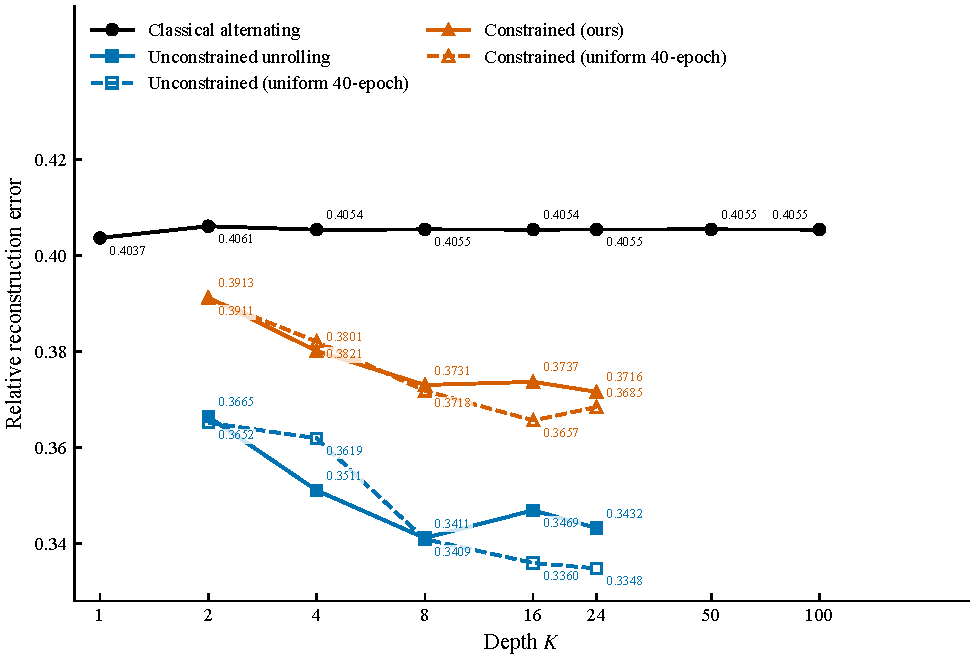
\includegraphics[width=\linewidth]{figures/fig_depth.pdf}
\caption{$100$ 个未见无噪声样本上、相对重建误差对深度 $K$ 的曲线。画框跨越完整实测范围，因此每个臂在其整个深度范围内都可见。两种展开变体在每个所示深度处都低于经典迭代的最佳值，且每个实测点都标出其数值；每个存档臂与其统一 $40$-epoch 重放被偏置到曲线的两侧，因为二者在 $K\le8$ 处重合到 $0.003$ 之内，否则会打印在一起。}
\label{fig:depth}
\end{figure}
\begin{table}[htbp]
\centering
\caption{经调谐的经典基线：最佳阻尼 $\alpha=\gamma$ 与相应的测试 RRE，在四种深度下对 $\alpha\in[0.1,1]$ 扫描，于 $100$ 个测试样本上。}
\label{tab:cls}
\begin{tabular}{lcc}
\toprule
深度 $K$ & 最佳 $\alpha=\gamma$ / RRE \\
\midrule
$8$   & $\numv{\NumClsSweepKEight}$ \\
$24$  & $\numv{\NumClsSweepKTwoFour}$ \\
$50$  & $\numv{\NumClsSweepKFifty}$ \\
$100$ & $\numv{\NumClsSweepKHundred}$ \\
\bottomrule
\end{tabular}
\end{table}
图~\ref{fig:depth} 显示测试 RRE 对深度的曲线。经典交替迭代几乎立即停滞：$\numv{\NumClassOne}$ 于 $K=1$，其整个范围上的最佳值 $\numv{\NumClassBest}$ 于 $K=\numv{\NumClassBestK}$，以及 $\numv{\NumClassHundred}$ 于 $K=100$，一个平台而非收敛。调谐其阻尼不改变图景，如表~\ref{tab:cls} 所示：即便整个网格上的最佳配置也只有 $\numv{\NumClsSweepBest}$（于 $\numv{\NumClsSweepBestK}$），相对未调谐设定仅增益 $\numv{\NumClsSweepGain}$。展开网络以远少的外部迭代达到可比较的误差：约束网络在 $K=\numv{\NumConsBestK}$ 处达到 $\numv{\NumConsBest}$（在 $K=2$ 处已达 $\numv{\NumConsTwo}$），无约束变体在 $K=\numv{\NumUncBestK}$ 处达到 $\numv{\NumUncBest}$；在 $K=8$ 处各数为 $\numv{\NumConsEight}$、$\numv{\NumUncEight}$ 与 $\numv{\NumClassEight}$。一个被认证的 $K=8$ 约束网络因此在 $K=8$ 处达到一个\emph{低于}经典迭代在其每个被测深度上最佳值的误差（$\numv{\NumConsEight}$ 对 $\numv{\NumClassBest}$，于 $K=\numv{\NumClassBestK}$）；对照经典 $K=100$ 运行（$\numv{\NumClassHundred}$）测量，同一网络以约 $12\times$ 更少的\emph{外部迭代}（在匹配逐层代价下）使用。比较的单位是迭代次数而非墙钟时间，且两个臂在关键处匹配：二者执行相同的正则化最小二乘对比度求解、具有相同的共轭梯度预算（$n_{\mathrm{cg}}=\numv{\NumNCg}$，第~\ref{sec:exp} 节），因此一个经典步与一层展开层只差在已学习模块。该模块并非免费：在生产形状上实测，它把逐层代价中位数墙钟提高到经典层的 $1{+}\numv{\NumCostLayerOverhead}$ 倍（附加费 $\numv{\NumCostLayerOverheadPct}\%$，或解析乘—加计数中的 $\numv{\NumCostMacOverheadPct}\%$），修正 CNN 本身占一个已学习层的 $\numv{\NumCostCnnPct}\%$，CG 求解占 $\numv{\NumCostCgPct}\%$。$12\times$ 迭代缩减因此在约 $1.4\times$ 量级的逐层附加费下以宽裕存活，但可辩护的论断是在匹配逐层代价下的迭代次数，即我们所报告的。主要基线是被阻尼交替不动点迭代，这些架构的经典祖先。还运行了两个更强的经典求解器，以使比较不依赖于弱参照：对比度源反演（CSI）\cite{csi_lit}，它交替对比度源（一个由 CG 解的线性最小二乘步）与经典 CSI 泛函上的逐点对比度更新；以及子空间优化方法（SOM）\cite{som_lit}，它从数据方程固定 $G_s$ 的主导右奇异子空间上的诱导电流，并通过状态方程优化其余部分。二者都从与展开网络\emph{相同的} Born-LS 初始化出发（测试 RRE $\numv{\NumBornInitRre}$）并运行到 $K=100$ 次外部迭代。

SOM 是一个真正强的参照：其最佳测试误差为 $\numv{\NumSomBest}$（于 $K=\numv{\NumSomBestK}$，子空间维数 $M=\numv{\NumSomBestM}$），远低于调谐阻尼迭代的 $\numv{\NumClsSweepBest}$，因此比较不依赖于弱参照。CSI 在此问题上收敛更慢，在 $K=8$ 处达 $\numv{\NumCsiAtKEight}$，在 $K=\numv{\NumCsiBestK}$ 处达 $\numv{\NumCsiBest}$，且在匹配深度处被约束网络击败。对 SOM，图景较不有利。在匹配深度 $K=8$ 处，约束网络达 $\numv{\NumConsEight}$，对照 SOM 的 $\numv{\NumSomAtKEight}$（在 $M$ 上最佳，此处 $M=\numv{\NumSomAtKEightM}$）；边距 $\numv{\NumSomMargKEight}$ 落在实测重跑地板 $\numv{\NumRepFloorMaxRre}$ \emph{以下}，因此在此深度两者不可区分，我们不声称获胜。在整个范围上 SOM 的最佳 $\numv{\NumSomBest}$ 比约束网络的最佳 $\numv{\NumConsBest}$ 低 $\numv{\NumSomMargBest}$，即在其最佳处 SOM 是更精确的方法；被认证网络的贡献在于它是唯一携带显式有界性证书、而非最精确的变体。无约束变体是被测方法中最精确的。子空间维数如同表~\ref{tab:cls} 的阻尼，是在发布版的网格 $M\in\{\numv{\NumSomMGrid}\}$ 上选取的。可辩护的论断是匹配深度的那一个，我们不声称墙钟获胜，下面的逐层代价核算成立，且只在匹配外部迭代深度处的精度。作为尺度参考，同一 $100$ 个样本上到 $K=100$ 的一次完整扫描的实测墙钟为 CSI $\SI{\numv{\NumCsiSecHundred}}{\second}$、SOM 在 $M=6$ 处 $\SI{\numv{\NumSomSecHundred}}{\second}$；展开臂在不同批大小下逐层计时，因此此处不把迭代比转换为加速。约束曲线在每个被测深度处都下降并在 $K=16$ 前饱和，如深度分解所预测——一个几何深度项加一个修正地板。存档曲线显示的从 $K=16$ 到 $K=24$ 的 $\numv{\NumDepDeltaArchPct}\%$ 上升，一旦每个深度都在统一调度下训练就\emph{不}复现，在同一区间读为 $\numv{\NumDepUniConsSixteen}\!\to\!\numv{\NumDepUniConsTwentyFour}$，即 $\numv{\NumDepDeltaUniPct}\%$；因此我们不再把此曲线描述为非单调的。无论如何该区间是未分辨的，因为\emph{两个}臂的变化都低于实测重跑地板（$\numv{\NumDepUniFloor}$，无约束臂事实上移动了 $\numv{\NumDepDeltaUncUniPct}\%$），因此我们的饱和论断是关于\emph{可分辨性}的，因为超出 $K=16$ 没有任何变化能在仪器噪声之上被分辨，而非一条严格单调性论断。无约束变体在每个被测深度处都更精确，超出 $\numv{\NumPriceDeltaLo}$--$\numv{\NumPriceDeltaHi}$（在 $K=8$ 处为 $\numv{\NumPriceDelta}$），即预算的代价，在第~\ref{sec:price} 节讨论。这些是受控小孔径设定（$8$ 次照明）下的\emph{相对}比较：约 $0.4$ 的绝对误差地板由温和照明与对比度步的正则化设定，而非由展开，且不被提议为竞争性成像结果。

\subsection{被认证与实测的谱量}

\emph{可复现性。} 表~\ref{tab:cert} 中的每个量都由一个单一审计驱动产生。其前向算子乘积是精确的（\texttt{torch.func.jvp}），其伴随是精确的逆向模式导数，二者都包裹在一个无矩阵算子中，因此没有任何谱估计被有限差分截断污染：$\sigma_{\max}$ 由 $J^{\!\top}\!J$ 上的 Lanczos/IRAM 获得，谱半径由 $J$ 上的 IRAM 获得，瞬态因子 $\sup_m\|J^m\|$ 由 $(J^{\!\top})^mJ^m$ 上的本征问题获得。幂迭代仅作为独立的旁证保留；由于两个估计量都是严格的下界，它们的分歧度量的是离散化散布而非数值。报告三个\emph{精确}自检。(i) 在一个随机线性测试映射上，把估计量与 \texttt{torch.linalg.matrix\_norm} 返回的精确奇异值比较（相对误差 $\numv{\NumInstrErr}$）。(ii) 在层本身上，把实测耦合块与引理~\ref{lem:blocks} 的闭式 $\sigma_{\max}(C)=\theta\alpha\mathcal{E}$ 比较（实测对证明的比值 $\numv{\NumSigCRatio}$）。(iii) 在 Born 变体中，其对比度步不依赖于场状态，两个块解析透明：$\sigma_{\max}(B)\equiv0$ 与 $\sigma_{\max}(A)=1-\gamma$，且仪器复现二者（$\numv{\NumBornSigmaB}$ 与 $\numv{\NumBornSigmaA}$）。在忠实变体中 $\sigma_{\max}(A)$ 没有闭式，对比度步通过场链 $\chi\to w^+\to E$ 依赖于 $\chi$，因此那里 $A$ 作为实测量报告而从不作为证书使用。表~\ref{tab:cert} 报告的块 $A$--$D$、全层 Jacobian 与 $\alpha$-扫描都以双精度计算，逐层修正审计与 $\chi$-行审计亦然；存档中唯一的单精度记录是被取代的遗留文件，在引用处标注为如此。原因是对比度步求逆一个 Tikhonov 系统，其最小特征值为 $\lambda_{\min}=\numv{\NumLamMin}$，因此穿过 $n_{\mathrm{cg}}=\numv{\NumNCg}$ 步 CG 循环的单精度方向导数会丢失有效数字；作为记录性例证，在两个精度分歧最大的步长处（$\alpha=\numv{\NumPrecAlphaWorst}$），单精度估计量返回 $\sigma_{\max}=\numv{\NumSigSingleWorst}$，对照双精度的 $\numv{\NumSigDoubleWorst}$。精度升级本身是可验证而非假设的：两个精度之间算子一致到 $\numv{\NumOpPrecRel}$，而同一状态上施加一层相差 $\numv{\NumLayerPrecAmp}$——即 $n_{\mathrm{cg}}$ 步 CG 求解放大了一个 $\numv{\NumOpPrecRel}$ 的算术差异。该单精度值保留在存档结果中作为假象证据，而非被使用。这些推导、本文带编号的论断与实现它们的函数之间的映射记录在数据可用性声明给出的仓库中。块记号是引理~\ref{lem:blocks} 的；\emph{已证明}/\emph{已实测}标签的含义在表~\ref{tab:cert} 图注中陈述。对比度路径行（$A$、$B$、层范数）在\emph{收敛}对比度求解处引用，已实现 $n_{\mathrm{cg}}=\numv{\NumNCg}$ 的值在第~\ref{sec:exp} 节（收敛控制）单独列出；场量 $\mathcal{E}=\numv{\NumEColMax}$ 与 $\alpha_c=\numv{\NumAlphaC}$ 在同一收敛求解处读取，即来自 $n_{\mathrm{cg}}$-扫描驱动，它是与表~\ref{tab:grid} 的网格研究不同的驱动与对比度样本。复合行（$\rho_\chi$、$\rho$、$M_J$、缺口、复合 $\sigma_{\max}$）在来自双精度复合审计的\emph{训练逐层}步长处求值，是与逐层行不同的算子。第 1 行是一个量显示在两列，因为设计值与证书是同一表达式，而非两个独立检查。$\Lambda$ 行只引用 \eqref{eq:Lambda} 的\emph{场}项；由谱裁剪得 $\prod_i\norm{W_i}_2\le1$，被省略的加性项至多为 $\norm{\mathbf{G}_s}_2\bar\epsilon/s_{\mathrm{res}}=\numv{\NumLamCorrTerm}$，即场项的 $\numv{\NumLamCorrRatio}$，因此列表值是场项而真实界为 $\Lambda\le\numv{\NumLambdaBound}+\numv{\NumLamCorrTerm}$。表~\ref{tab:cert2} 收集在训练步长处测量的复合、保真度与噪声行。两个驱动组不是逐项可比的；其来源记录如下。

\begin{table}[htbp]
\centering
\caption{训练层映射的块与阈值。“已证明”条目是在实测工作点处的严格不等式，可作为定理假设；“已实测”条目是数值记录且\emph{不}用作假设。破折号：该列对该行不适用。}
\label{tab:cert}
\footnotesize\setlength{\tabcolsep}{4pt}
\begin{tabular}{@{}p{0.34\textwidth}p{0.20\textwidth}p{0.13\textwidth}p{0.20\textwidth}@{}}
\toprule
块 / 量 & 闭式 & 已证明 & 已实测 \\
\midrule
$D$：定理~\ref{thm:field} 的场块 $\sigma_{\max}$ & $1-\alpha(1-\beta_0)=\numv{\NumGammaW}$ & $=\numv{\NumThmFieldD}$ & $\numv{\NumPhysWBlock}$ \\
$C$：引理~\ref{lem:blocks} 的耦合块 & $\alpha\mathcal{E}=\numv{\NumSigCLower}$ & $\numv{\NumSigCLower}$ & $\numv{\NumSigC}$ \\
\quad 作为 $\sigma_{\max}(J)$ 的下界 & $\alpha\mathcal{E}$ & $\numv{\NumSigLowBound}$ & \textemdash \\
$A$：对比度块 $\sigma_{\max}$ & \textemdash & \textemdash & $\numv{\NumSigA}$ \\
$B$：修正侧耦合 $\sigma_{\max}$ & \textemdash & \textemdash & $\numv{\NumSigB}$ \\
峰值场列范数 $\mathcal{E}$ / $\ell_\infty$ 比值 & $\max_r\norm{E_{\cdot,r}}_2$ & \textemdash & $\numv{\NumEColMax}$ / $\numv{\NumEInfRatio}$ \\
非收缩阈值 $\alpha_c=(\theta\mathcal{E})^{-1}$ & $(\theta\mathcal{E})^{-1}$ & $\numv{\NumAlphaC}$ & \textemdash \\
物理核 $\sigma_{\max}(J)$，无修正 & \textemdash & \textemdash & $\numv{\NumPhysSigma}$ \\
Born 对比度变体，强制 $B\equiv0$ & \textemdash & \textemdash & $\numv{\NumBornSigmaFull}$ \\
$\operatorname{Lip}(H_k)$，斜率预算 $\ell$ & \textemdash & \textemdash & $\numv{\NumLipHCons}$ / $\numv{\NumLipHUnc}$ \\
\bottomrule
\end{tabular}
\end{table}

\begin{table}[htbp]
\centering
\caption{复合、保真度与噪声量。除非列另有说明，所有条目都在训练步长处实测；推论~\ref{cor:fidelity} 的 $\rho_\chi$ 假设在无约束臂中被否定、在约束臂中未被决定。}
\label{tab:cert2}
\footnotesize\setlength{\tabcolsep}{4pt}
\begin{tabular}{@{}p{0.40\textwidth}p{0.14\textwidth}p{0.30\textwidth}@{}}
\toprule
量 & 状态 & 值 \\
\midrule
已实现求解处的对比度路径块 $A$ / $B$ / $J$ & 实测 & $\numv{\NumSigAImpl}$ / $\numv{\NumSigBImpl}$ / $\numv{\NumSigmaFullImpl}$ \\
复合 $\sigma_{\max}$，$K{=}8$ 循环 & 实测 & $\numv{\NumSigCompCons}$ / $\numv{\NumSigCompUnc}$ \\
\quad 固定 $\alpha=\gamma=\tfrac12$ 的逐层复合，\emph{按实现}（$n_{\mathrm{cg}}=\numv{\NumNCg}$；收敛对 $\numv{\NumGdPhysSigmaConv}$ / $\numv{\NumSigCompLayerConsConv}$） & 实测 & $\numv{\NumSigCompLayerCons}$ / $\numv{\NumSigCompLayerUnc}$ \\
$\rho_\chi$ = $\chi\!\to\!\chi$ 块的 $\sigma_{\max}$，即 $\chi$-映射 Lipschitz 常数的一个\emph{下}界 & 实测 & $\numv{\NumRhoChiCons}$ / $\numv{\NumRhoChiUnc}$ \\
\quad $\hat G$ 的 $\chi$-映射 Lipschitz 常数，行块 $[A\,B]$ & 实测 & $\numv{\NumChiLipRowCons}$ / $\numv{\NumChiLipRowUnc}$ \\
\quad 物理映射 $F$（$H\equiv0$），行块 $[A\,B]$ & 实测 & $\numv{\NumChiLipRowFCons}$ / $\numv{\NumChiLipRowFUnc}$ \\
\quad 物理映射 $F$，$\chi\!\to\!\chi$ 块 & 实测 & $\numv{\NumChiFBlockCons}$ / $\numv{\NumChiFBlockUnc}$ \\
\quad 物理映射 $F$，谱半径，已学习步长 & 实测 & $\numv{\NumChiRhoFCons}$ / $\numv{\NumChiRhoFUnc}$ \\
\quad 固定 $\alpha=\gamma=\tfrac12$ 处相同 & 实测 & $\numv{\NumChiRhoFFixCons}$ / $\numv{\NumChiRhoFFixUnc}$ \\
\quad 同一块，谱半径而非 Lipschitz 常数 & 实测 & $\numv{\NumRhoChiSpecCons}$ / $\numv{\NumRhoChiSpecUnc}$ \\
瞬态 $M_J=\max_{m\le2}\norm{J^m}$（推论~\ref{cor:noisenormal} 的深度-2 截断） & 实测 & $\numv{\NumMJCons}$ \\
\quad 在完整视界 $m\in\{1,2,4,8\}$ 上的相同：截断并非良性 & 实测 & $\numv{\NumMJFullCons}$ ($m{=}\numv{\NumMJFullArgmaxM}$) / $\numv{\NumMJFullUnc}$ ($m{=}\numv{\NumMJFullArgmaxMUnc}$) \\
非正规性缺口 $\sigma_{\max}/\rho$ & 实测 & $\numv{\NumGapRatio}$ \\
噪声增益 $\Lambda$（数据$\to\chi$ 通道）：\eqref{eq:Lambda} 的场项 & 实测 & $\numv{\NumLambdaMeas}$，以 $\numv{\NumLambdaBound}+\numv{\NumLamCorrTerm}$ 为界 \\
\bottomrule
\end{tabular}
\end{table}
\emph{来源。} 所有行都由在 Born--LS 初始状态、固定 $\alpha=\gamma=1/2$、投影开、float64 下的单一审计驱动产生；$K{=}8$ 循环行使用在已学习步长处的独立驱动。已实现的 $n_{\mathrm{cg}}$ 值只在与收敛求解值不同的对比度路径块上；与 CG 无关的块 $C$ 与 $D$ 在扫描上逐位相同，这正是使证书与 CG 无关的原因。单精度重跑因主导三元组未被分辨而把对比度路径奇异值高估数量级；此处所有列表值都是双精度。

四点结论。(1) 场块在 $\numv{\NumPhysWBlock}$ 处收缩，低于先验界 $1-\alpha(1-\beta_0)=\numv{\NumGammaW}$：定理~\ref{thm:field} 的证书有效但保守。(2) 耦合块是障碍且以闭式可用：$\sigma_{\max}(C)=\alpha\mathcal{E}=\numv{\NumSigCLower}>1$，阈值 $\alpha_c=\numv{\NumAlphaC}<\tfrac12$，因此在工作步长处非收缩性被\emph{证明}而非仅被观测。(3) 对比度路径块给出 $\sigma_{\max}(A)=\numv{\NumSigA}$ 与 $\sigma_{\max}(B)=\numv{\NumSigB}$；$\hat G$ 的 $\chi$ 行在约束臂中测得 $\numv{\NumRhoChiCons}$ 与 $\numv{\NumChiLipRowCons}$，二者都低于一，而在无约束臂中为 $\numv{\NumChiLipRowUnc}$，后者在该处否定 $\rho_\chi<1$。两个臂都不产生被认证的漂移半径，因此推论~\ref{cor:fidelity} 作为条件性论断报告。(4) 复合增益在每个被测配置中都超过一，但闭式耦合块 $\sigma_{\max}(C)=\alpha\mathcal{E}>1$ 已经对任何修正强制 $\sigma_{\max}(DT_k)>1$（命题~\ref{prop:imposs}）。双线性耦合 $\chi\odot E$ 使忠实复合无论修正如何被控制都非收缩，这正是我们提供的保证是有界性与逐层核算、而非逐层收缩速率的原因。

\subsection{长程外推与防护栏}
\label{sec:extrap}
\begin{figure}[htbp]
\centering
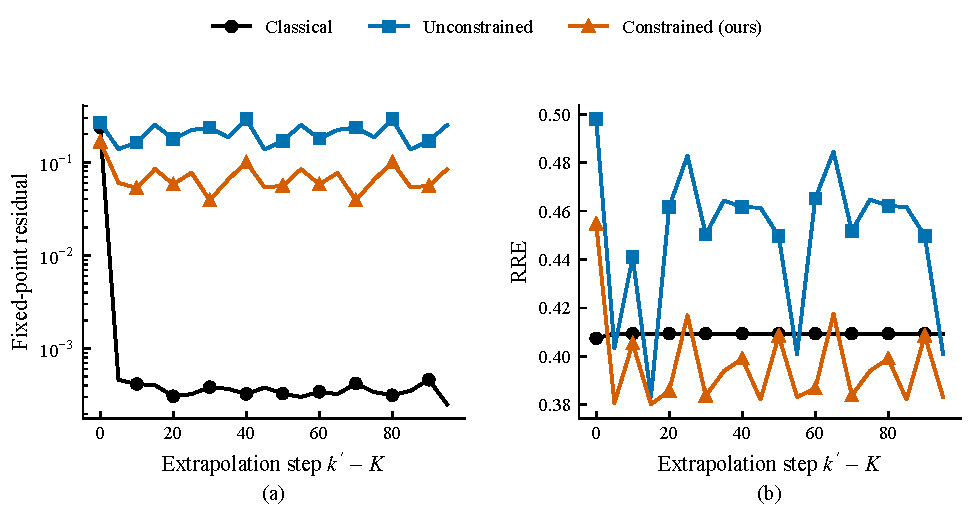
\includegraphics[width=\linewidth]{figures/fig_extrap.pdf}
\caption{训练所得 $K=8$ 层的循环深度外推（$100$ 个附加步）：(a) 不动点残差；(b) 重建误差。}
\label{fig:extrap}
\end{figure}
$\infn{\chi}$ 是视界上所达到的最大对比度幅值；$\beta_0=\infn{\chi}\norm{\mathbf{G}_b}_2$ 是所得先验常数。

\begin{figure}[htbp]
\centering
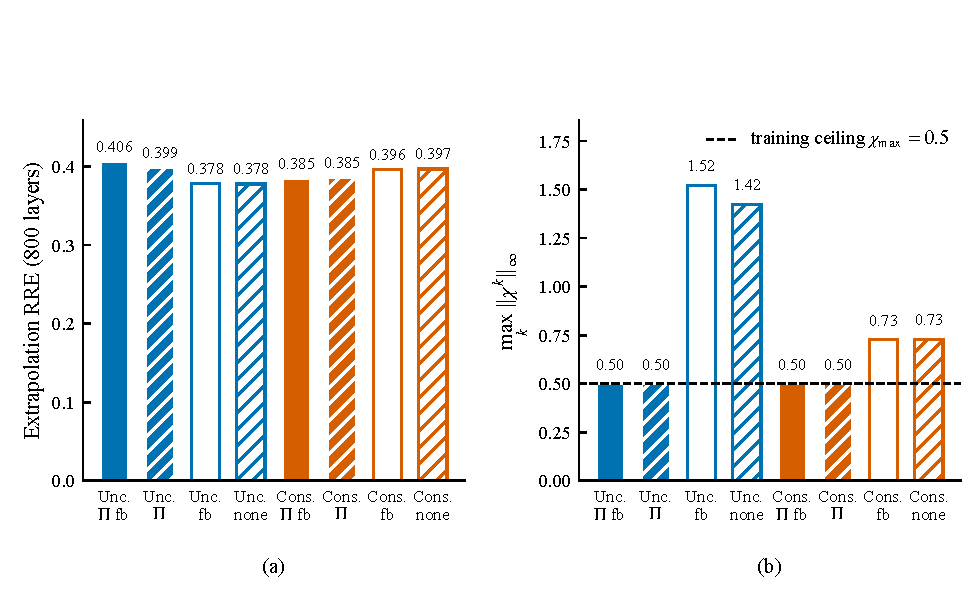
\includegraphics[width=\linewidth]{figures/fig_ablation.pdf}
\caption{消融~I：(a) 重建误差与 (b) $800$ 个展开层后的训练对比度上限，于图~\ref{fig:depth} 的无噪声集上。色相给出族，填充给出投影标志，阴影给出特征边界，每个柱下的文字重复组合；每个柱都标出其数值。}
\label{fig:abl}
\end{figure}
\begin{figure}[htbp]
\centering
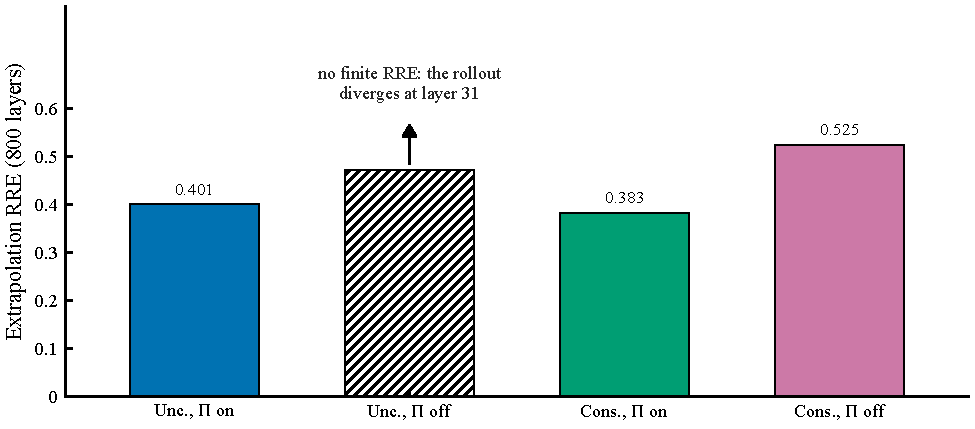
\includegraphics[width=\linewidth]{figures/fig_frozen.pdf}
\caption{消融~II：$800$ 层、在测试时从冻结权重去掉 $\Pi$ 后的外推误差，同一集合，线性尺度。阴影主干是发散的运行，其顶部刻意不标数值；其他列上的数字是列表误差。}
\label{fig:frozen}
\end{figure}
图~\ref{fig:extrap} 把训练所得 $K=8$ 层循环重复 $100$ 个附加步（$800$ 层）。两个展开网络都不单调收缩。约束残差从第一步的 $\numv{\NumResConsTrans}$ 落入一个窄极限环，然后在剩余视界内于 $[\numv{\NumResConsBandLo},\numv{\NumResConsBandHi}]$ 中振荡——在代表性一步处为 $\numv{\NumResConsHead}$，在最后记录步处为 $\numv{\NumResConsEnd}$，该记录每五步采样一次——且 $\infn{\chi}$ 钉在 $\numv{\chimax}$，因此其重建误差保持有界。无约束残差也\emph{不是}单调的，且引用其端点会低估它：它在环内尖峰到 $\numv{\NumResUncSpike}$，比约束带高出一个数量级以上，而 $|\chi|$ 仍被 $\Pi$ 夹紧。因此漂移在残差中可见而非在状态中；经典迭代驻留在其自身不动点（残差 $\approx\numv{\NumResClsEnd}$）。

\begin{table}[htbp]
\centering
\caption{消融~I：对训练时标志的完整 $2\times2\times2$ 析因，运行 $800$ 个展开层；除所列标志外，种子与训练调度相同。破折号标记不适用于该臂的标志。}
\label{tab:abl}
\begin{tabular}{llcccc}
\toprule
修正 & $\Pi$ & 特征边界 & 外推 RRE & $\infn{\chi}$ & $\beta_0$ \\
\midrule
经典 & --- & --- & $\numv{\NumAblClsProjOn}$ & $\numv{\NumAblClsChi}$ & $\numv{\betacert}$ \\
无约束  & 开  & 开  & $\numv{\NumAblUncPOnFbOnRre}$ & $\numv{\NumAblUncPOnFbOnChi}$ & $\numv{\NumBetaUncPOnFbOn}$ \\
无约束  & 开  & 关 & $\numv{\NumAblUncPOnFbOffRre}$ & $\numv{\NumAblUncPOnFbOffChi}$ & $\numv{\NumBetaUncPOnFbOff}$ \\
无约束  & 关 & 开  & $\numv{\NumAblUncPOffFbOnRre}$ & $\numv{\NumAblUncPOffFbOnChi}$ & $\numv{\NumBetaUncPOffFbOn}$ \\
无约束  & 关 & 关 & $\numv{\NumAblUncPOffFbOffRre}$ & $\numv{\NumAblUncPOffFbOffChi}$ & $\numv{\NumBetaUncPOffFbOff}$ \\
约束 & 开  & 开  & $\numv{\NumAblConsPOnFbOnRre}$ & $\numv{\NumAblConsPOnFbOnChi}$ & $\numv{\NumBetaConsPOnFbOn}$ \\
约束 & 开  & 关 & $\numv{\NumAblConsPOnFbOffRre}$ & $\numv{\NumAblConsPOnFbOffChi}$ & $\numv{\NumBetaConsPOnFbOff}$ \\
约束 & 关 & 开  & $\numv{\NumAblConsPOffFbOnRre}$ & $\numv{\NumAblConsPOffFbOnChi}$ & $\numv{\NumBetaConsPOffFbOn}$ \\
约束 & 关 & 关 & $\numv{\NumAblConsPOffFbOffRre}$ & $\numv{\NumAblConsPOffFbOffChi}$ & $\numv{\NumBetaConsPOffFbOff}$ \\
\bottomrule
\end{tabular}
\end{table}
\begin{table}[htbp]
\centering
\caption{消融~II，推理时从\emph{用} $\Pi$ 训练的\emph{冻结}权重去掉 $\Pi$（$K=8$；RRE 指短视界 / $800$-层外推）。“div.” 标记在到达视界前离开有限范围的展开轨迹，因此没有可引用的外推误差。}
\label{tab:abl2}
\begin{tabular}{llccc}
\toprule
冻结权重 & 测试时 $\Pi$ & 短程 RRE & 外推 RRE & $\infn{\chi}$ \\
\midrule
无约束 & 开  & $\numv{\NumFrzUncOnShort}$ & $\numv{\NumFrzUncOn}$ & $\numv{\chimax}$ \\
无约束 & 关 & $\numv{\NumFrzUncOffShort}$ & $\numv{\NumFrzUncOff}$ & $\numv{\NumFrzUncOffChi}$ \\
约束   & 开  & $\numv{\NumFrzConsOnShort}$ & $\numv{\NumFrzConsOn}$ & $\numv{\chimax}$ \\
约束   & 关 & $\numv{\NumFrzConsOffShort}$ & $\numv{\NumFrzConsOff}$ & $\numv{\NumFrzConsOffChi}$ \\
\bottomrule
\end{tabular}
\end{table}
\noindent
表~\ref{tab:abl}--\ref{tab:abl2} 显示哪一种成分负责哪一种性质。每个成分都从承载其理论角色的量读出，而非从单一误差列：投影通过对比度上限 $\infn{\chi}$（在每个有它的臂中钉在 $\chi_{\max}$、在每个没有它的臂中离开盒子）读出；振幅预算通过相对 $\bar\epsilon$ 的实现修正读出；特征边界通过使 $\bar\epsilon$ 可实现的躯干输入范围读出；谱裁剪通过模块范数读出，并以在固定预算下没有稳定性增益的方式负面读出；CG 预算通过第~\ref{sec:cgsweep} 节记录的残差与块漂移读出。两表回答\emph{不同}问题，并非同一效应的两个估计。消融~II 固定权重并在推理时去掉 $\Pi$——同一初始状态、同一 $K{=}8$ 块重复到 $800$ 层、无重训练——因此它隔离投影对一个以它训练的轨迹所做的什么。消融~I 从零重训练每个臂且 $\Pi$ 关闭，并问训练能否找到一个无它的稳定参数集。第二种中的有界结果是训练所落参数集的经验性质，且不带任何先验证书；因此二者绝不被合并为关于投影必要性的单一论断。

\emph{(a) 投影在推理时不可或缺。} 表~\ref{tab:abl2}、图~\ref{fig:frozen} 的消融~II 从\emph{用 $\Pi$ 训练的}冻结权重中去掉 $\Pi$，是最干净的单变量测试。无约束网络的误差已在短视界处从 $\numv{\NumFrzUncOn}$ 跳到 $\numv{\NumFrzUncOffShort}$，且其 $800$-层展开轨迹在第 $\numv{\NumFrzUncBreak}$ 层离开有限范围，$\infn{\chi}$ 达到 $\numv{\NumFrzUncOffChi}$：状态以两个数量级离开容许集且迭代不返回。约束网络退化但存活（$\numv{\NumFrzConsOff}$），因为其修正被 $\bar\epsilon$ 限界且不能把状态推远。这是定理~\ref{thm:bounded} 的操作性论断：投影不是装饰性夹紧。

\emph{(b) 重训练能掩盖问题，但代价是证书。} 表~\ref{tab:abl}、图~\ref{fig:abl} 的消融~I 显示，一个\emph{训练时}无 $\Pi$ 的网络重新学习一个碰巧保持有界的个工作点（$\numv{\NumAblUncPOffFbOnRre}$ 对带 $\Pi$ 的 $\numv{\NumAblUncPOnFbOnRre}$，差 $\numv{\NumAblProjDelta}$）。表~\ref{tab:abl} 的经典行没有已学习修正、没有投影标志也没有特征边界标志，且由于其对比度饱和上限 $\chi_{\max}=\numv{\chimax}$，其 $\beta_0$ 是被认证的 $\chi_{\max}\norm{\mathbf{G}_b}_2=\numv{\betacert}$ 而非单独实测值。它不保留的是界：实测 $\infn{\chi}=\numv{\NumAblUncPOffFbOnChi}$ 给出 $\beta_0^{\mathrm{meas}}=\numv{\NumBetaMeas}>1$，因此定理~\ref{thm:bounded} 的假设失效，有界性退化为关于一个训练参数集的经验观察。这正是展开文献当前未做的区分，也是保留 $\Pi$ 的实践原因：\emph{靠运气的有界性 vs 靠构造的有界性}。

\emph{(c) 防护栏实际买来什么：关于误差作为代理的一个否定结果。} 没有任何臂离开浮点范围：全部八个臂在整个视界上都是数值有限的。各臂由\emph{状态}而非误差区分。有 $\Pi$ 时，$\infn{\chi}$ 在每个臂中都钉在 $\numv{\chimax}$；无 $\Pi$ 时它达到 $\numv{\NumAblUncPOffFbOnChi}$--$\numv{\NumAblUncPOffFbOffChi}$，即它离开容许盒而重建误差仍有限，且事实上略\emph{低}：$\numv{\NumAblUncPOffFbOnRre}$ 对 $\numv{\NumAblUncPOnFbOnRre}$，这是在投影开启、特征边界保持开启下的单变量比较。因此有限的误差\emph{不是}证书的证据：证书是关于状态的论断，且是投影、而非观测到的精度，强制了它。我们显式报告这一点，因为相反的读法——“无约束展开轨迹发散”——正是较早展开文献所报告、也是读者在此会预期的内容，而它不是我们数据显示的。特征边界因另一原因仍承重：它正是使振幅预算 $\bar\epsilon$ 可由构造达到的原因，如注记~\ref{rem:featscale} 所解释。

\emph{(d) 有界性读法不是单次运行假象。} 上面各臂针对一个训练种子报告，因此我们在每个臂上复制了其所依赖的对比度，跨 $\numv{\NumSeedNCons}$ 个训练种子（$\numv{\NumSeedNCons}$ 个约束，$\numv{\NumSeedNUnc}$ 个无约束，$\numv{\NumSeedNProjOff}$ 个去投影无约束），每个种子都是用自身数据与初始化种子的完整重训练。每个运行在整个视界上数值有限（$\numv{\NumSeedFinite}$）。约束臂在\emph{每个}种子处都停在 $\infn{\chi}=\numv{\NumSeedChiConsMax}$（钉在盒上），而去掉投影训练的各臂在每个种子处都离开它（$\infn{\chi}=\numv{\NumSeedProjOffBox}$）；因此分离是设计标志的性质，而非某次初始化。深度结论同样稳定：在这些运行中 $K{=}8$ 测试误差为 $\numv{\NumSeedRreMeanCons}\pm\numv{\NumSeedRreSdCons}$（约束）与 $\numv{\NumSeedRreMeanUnc}\pm\numv{\NumSeedRreSdUnc}$（无约束），其中第二项是总体标准差，且散布并非仅由均值承担：中位数为 $\numv{\NumSeedRreMedCons}$ 与 $\numv{\NumSeedRreMedUnc}$，上四分位数为 $\numv{\NumSeedRreHiCons}$ 与 $\numv{\NumSeedRreHiUnc}$，因此没有任何运行藏在尾部。同一运行上的 $800$-层外推误差为 $\numv{\NumSeedExMeanCons}\pm\numv{\NumSeedExSdCons}$ 与 $\numv{\NumSeedExMeanUnc}\pm\numv{\NumSeedExSdUnc}$。该标准差必须谨慎读，因为它通常被误认的那个量也已被测量。以\emph{相同}种子、\emph{相同}种子重跑同一驱动，两次存档间的训练路径逐字节相同，把 $K{=}8$ 误差移动至多 $\numv{\NumRepFloorMaxRre}$（中位 $\numv{\NumRepFloorMedRre}$）、把 $800$-层外推误差移动至多 $\numv{\NumRepFloorMaxExtrap}$，跨越两个存档中都存在的 $\numv{\NumRepNShared}$ 次运行。因此相同种子的地板\emph{不}小到可与跨种子散布相比，且我们不把后者作为此流水线的误差棒呈现。复制所确立的更窄：结论所依赖的两个论断在每次重复中都不变，每次运行都数值有限，且容许盒论断在所有 $\numv{\NumRepNShared}$ 个重叠运行中稳定（有限稳定：\numv{\NumRepFiniteStable}；盒稳定：\numv{\NumRepBoxStable}）。

因此实践建议强于“方便就投影”：投影加一个有界特征映射是把展开式逆散射从经验稳定的启发式转换为带有闭式不变集的迭代的两个成分；振幅预算随后提供推论~\ref{cor:fidelity} 的保真度半径。

\subsection{噪声稳定性}\label{sec:noise}

\emph{噪声协议。} 训练样本携带复高斯噪声。其 SNR 为 $\SI{20}{\decibel}$，定义为十倍以 10 为底的、所有接收机与入射通道上平均无噪声信号功率 $\mean|y^{0}|^{2}$ 对平均噪声功率 $\mean|n|^{2}$ 之比的对数；评估集（$100$ 个未见样本）由构造无噪声，因此深度与外推研究测量的是重建误差而非测量噪声；噪声在下面于 $\SI{30}{\decibel}$--$\SI{5}{\decibel}$ 显式注入。“无噪声”此处指合成 SNR 设为 $\SI{\numv{\NumNoiseNominalDb}}{\decibel}$，且我们不当字面值：$f$ 生成器以 float64 计算但\emph{交付}场为 complex64，因此存储数据所能表示的最安静信号是 complex64 表示误差。我们实测它（相对范数 $\numv{\NumNoiseFloorRel}$，有效地板在 $\SI{\numv{\NumNoiseFloorDb}}{\decibel}$），因此评估集只在其实测地板远低于随后注入的 $\SI{30}{\decibel}$--$\SI{5}{\decibel}$ 噪声的意义下无噪声；我们引用该地板而非请求值。
实线标记在\emph{收敛}对比度求解（$n_{\mathrm{cg}}=\numv{\NumNCgConv}$）处计算，与表~\ref{tab:cert} 匹配；浅灰系列是已实现 $n_{\mathrm{cg}}=\numv{\NumNCg}$ 扫描，仅作为第~\ref{sec:exp} 节所讨论假象的记录保留。图~\ref{fig:alphac} 绘制该扫描：它由跨越 $[0.05,1]$ 的 $\numv{\NumAlphaSweepN}$ 个 $\alpha=\gamma$ 值组成，且 $\mathcal{E}=\max_r\norm{E_{\cdot,r}}_2$ 列表于表~\ref{tab:cert}，因此 $\alpha_c=(\theta\mathcal{E})^{-1}$ 可由列表量单独重算。

\begin{figure}[htbp]
\centering
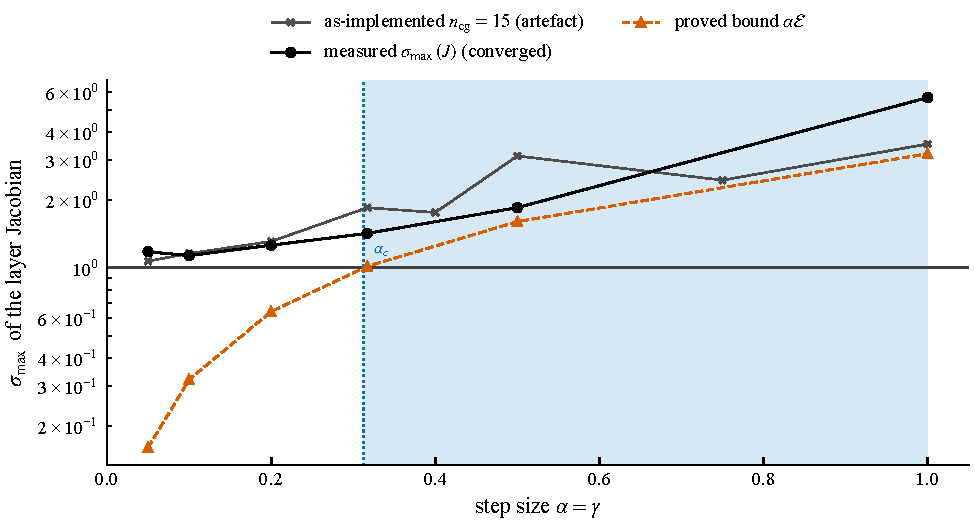
\includegraphics[width=\linewidth]{figures/fig_alphac.pdf}
\caption{物理核层 Jacobian 的实测 $\sigma_{\max}$ 对步长 $\alpha=\gamma$ 的曲线（标记），对照命题~\ref{prop:imposs} 的严格下界 $\alpha\mathcal{E}$（虚线）与阈值 $\alpha_c=(\theta\mathcal{E})^{-1}$（点线）。只有 $\alpha_c$ 右侧区域被证明。}
\label{fig:alphac}
\end{figure}
\begin{figure}[htbp]
\centering
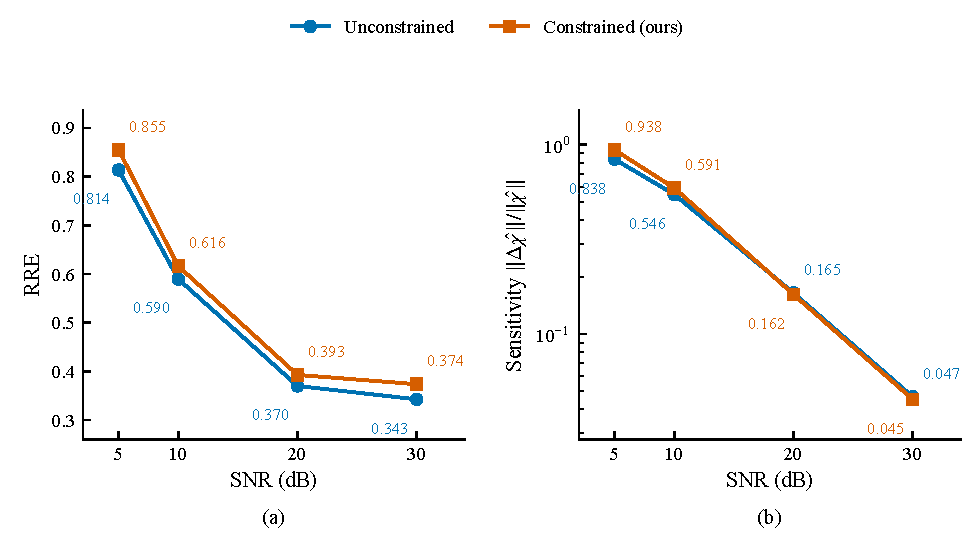
\includegraphics[width=\linewidth]{figures/fig_noise.pdf}
\caption{深度 $K=8$ 处的噪声敏感度：(a) 重建误差对 SNR 的曲线；(b) 输出扰动 $\norm{\hat\chi(y+\Delta y)-\hat\chi(y)}/\norm{\hat\chi(y)}$ 于每点 $100$ 个测试样本。每个标记都标出其数值。}
\label{fig:noise}
\end{figure}
图~\ref{fig:noise} 在从 $\SI{30}{\decibel}$ 到 $\SI{5}{\decibel}$ 的测量噪声下评估两个网络。两者都单调退化，且在 $\SI{20}{\decibel}$ 处的敏感度 $\numv{\NumSensCons}$（约束）对 $\numv{\NumSensUnc}$（无约束）相近：在此实验中振幅预算\emph{不}买来可见的噪声优势。预算所提供的不是形如 $\Lambda/(1-\rho)$ 的界（如上所示它是条件性的且此处假设为假），而是进入精确刻画 \eqref{eq:noiseexact} 的量 $\Lambda$ 与 $M_J$；这些可针对任何网格重算并可在训练中跟踪。我们把它作为一个显式的否定经验发现报告：约束族的价值在于可认证性与有界性，而非精度或实测鲁棒性，且此架构的噪声保证将需要注记~\ref{rem:averaged} 的平均构造（带其精度代价），或带实测 $\Lambda$ 与 $M_J$ 的有限深度部署。

\subsection{逐层增益与梯度}
这些是依赖于对比度路径的量，由实化 Jacobian 上的幂迭代计算，并在线性测试映射上对照精确 SVD 验证。

\begin{figure}[htbp]
\centering
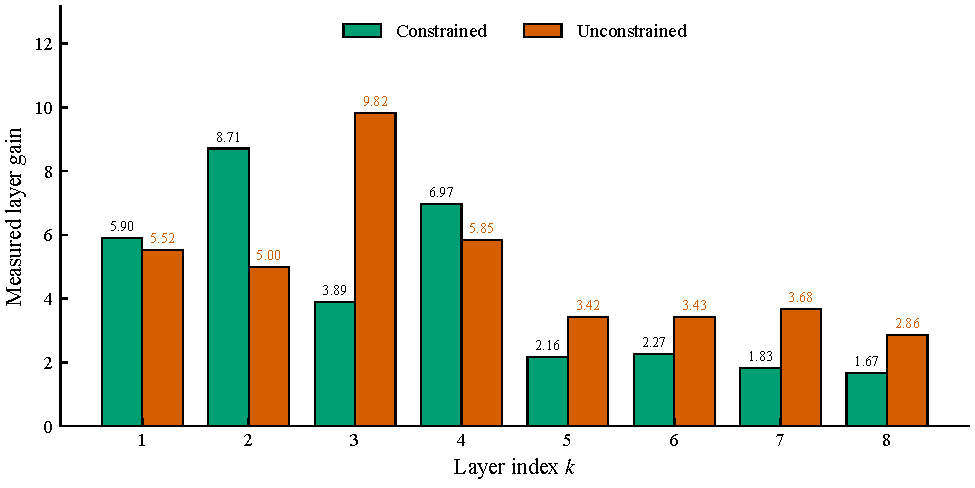
\includegraphics[width=\linewidth]{figures/fig_gain.pdf}
\caption{在已实现对比度路径（$n_{\mathrm{cg}}=\numv{\NumNCg}$）上、已学习步长处每层 Jacobian 的实测谱范数，每个柱上都印有数值。}
\label{fig:gain}
\end{figure}
\begin{figure}[htbp]
\centering
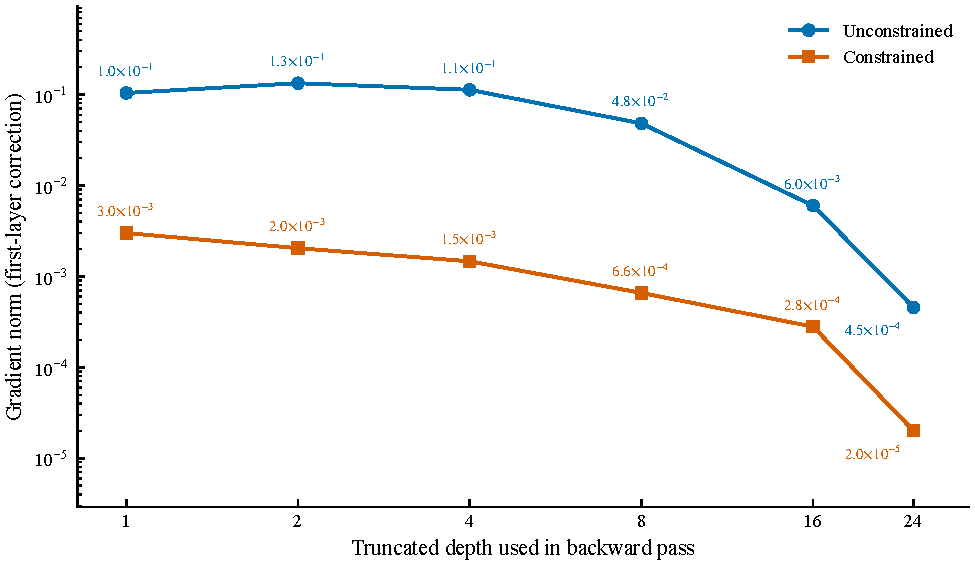
\includegraphics[width=\linewidth]{figures/fig_gradnorm.pdf}
\caption{对 $K=24$ 模型，第一层梯度范数对反向通路中所用截断深度的曲线。每个标记都标出其数值。}
\label{fig:gradnorm}
\end{figure}
在\emph{已学习}步长处（图~\ref{fig:gain}），两个变体在每层都超过一，且约束变体并非系统性更小，复合增益由物理核主导，其阻尼因子 $\alpha_k$ 本身是被学习的，且在约束运行中收敛到更大值（$\numv{\NumAlphaCons}$ 对 $\numv{\NumAlphaUnc}$）。这是一个混杂比较；表~\ref{tab:cert} 通过固定 $\alpha=\gamma=0.5$ 消除混杂。图~\ref{fig:gradnorm} 的梯度范数探针显示了预算在训练侧的对应物：在截断深度 $1$ 处，预算下第一层梯度范数为 $\numv{\NumGradConsOne}$，无预算时为 $\numv{\NumGradUncOne}$，且二者都随深度衰减，一种消失梯度效应，它内在于深度展开，且被约束参数化通过抑制有效步长而放大。这是保证的梯度健康代价。

\subsection{认证的代价}\label{sec:price}
\begin{figure}[htbp]
\centering
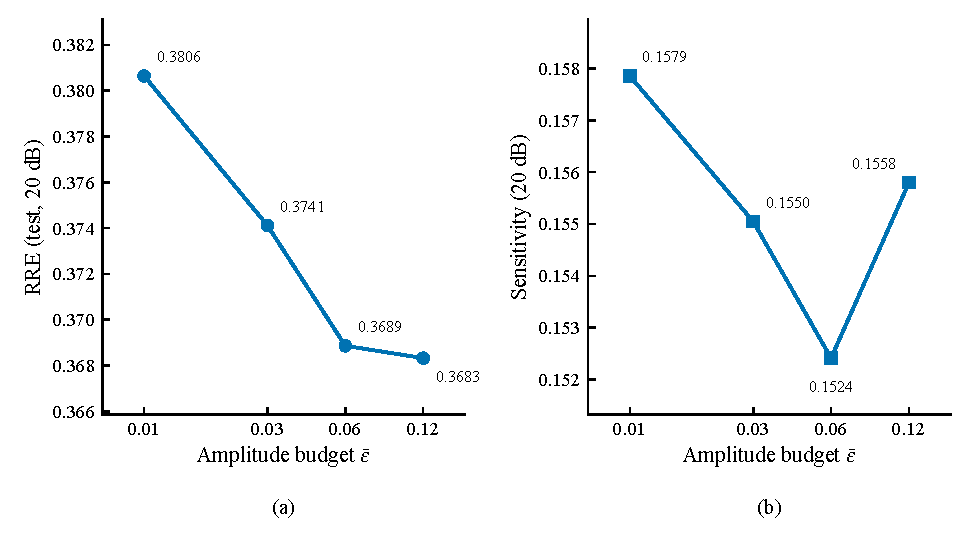
\includegraphics[width=\linewidth]{figures/fig_pareto.pdf}
\caption{$K=8$ 处、在 $\bar\epsilon$ 上跨越 12 倍因子的振幅预算扫描，在扫描预算处按对数轴绘制：(a) 精度；(b) 噪声敏感度。}
\label{fig:pareto}
\end{figure}
\begin{figure}[htbp]
\centering
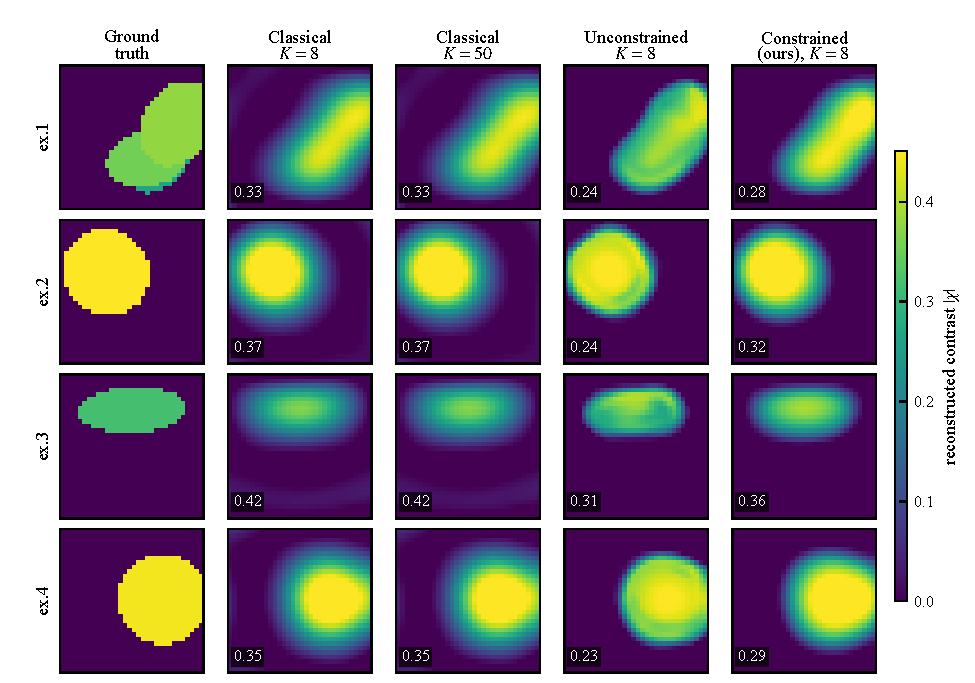
\includegraphics[width=\linewidth]{figures/fig_images.pdf}
\caption{测试集上一个颜色尺度下的重建示例。每个面板中的数字是该面板的相对误差 $\|\hat\chi-\chi\|_2/\|\chi\|_2$（越小越好），而非平方误差，因此视觉比较也是一种测量。每个标题给出方法与深度。两个已学习臂的区别在振幅预算而非投影；正文把其数字间的差距归因于文本。}
\label{fig:images}
\end{figure}
图~\ref{fig:pareto} 在 $K=8$ 处扫描 $\bar\epsilon$。误差与敏感度都随 $\bar\epsilon$ 从 $\numv{\NumEbWorst}$ 增至 $\numv{\NumEbBest}$ 而改善：在预算化族内部，约束是一个\emph{地板}而非优化器，且默认 $\bar\epsilon=\numv{\epsbar}$ 落在曲线的平坦部分。相关的权衡不在约束族内部，而在该族与无约束展开之间：图~\ref{fig:depth} 的精度差距 $\numv{\NumPriceDelta}$ 正是为一个有界性证书（定理~\ref{thm:bounded}）与场子系统速率（定理~\ref{thm:field}）连同表~\ref{tab:abl}--\ref{tab:abl2} 的审计所付出的。直白地说：无约束展开是更好的估计器，约束族是更好的\emph{制品}，它附带保修，而保修是有界性加可重算常数，而非命题~\ref{prop:imposs} 的收缩速率。图~\ref{fig:images} 显示测试重建。该图有一个容易被误读的特征。每个面板中的数字是一个距离，因此越小越好，且在每个示例上约束臂的数字都是两个中较大的（$\numv{\NumRreImgCons}$ 对这四个面板上的 $\numv{\NumRreImgUnc}$，全测试集上 $\numv{\NumConsEight}$ 对 $\numv{\NumUncEight}$）。这既非符号约定也非投影的效应。在表~\ref{tab:abl} 的 $K=8$ 析因中，振幅预算解释了差距的 $+\numv{\NumPriceBudget}$，而关闭投影在无约束臂中把误差移动 $-\numv{\NumPriceProjUnc}$、在约束臂中移动 $+\numv{\NumPriceProjCons}$，即符号不一致。该差距是预算 $\bar\epsilon$ 本身——即使定理~\ref{thm:bounded} 不变集显式的那个参数——的实测代价；它不买精度且不被呈现为精度。
作为不通过相对对比度误差的、图像域的检查，我们额外在图~\ref{fig:images} 显示的 $\numv{\NumNImg}$ 个示例上测量 PSNR 与 SSIM：约束网络达 $\numv{\NumPsnrCons}$~dB / SSIM~$\numv{\NumSsimCons}$，无约束网络 $\numv{\NumPsnrUnc}$~dB / SSIM~$\numv{\NumSsimUnc}$，经典 $K=8$ 与 $K=50$ 迭代为 $\numv{\NumPsnrClsEight}$ 与 $\numv{\NumPsnrClsFiveZero}$~dB、SSIM~$\numv{\NumSsimClsEight}$ 与 $\numv{\NumSsimClsFiveZero}$。排序与图~\ref{fig:depth} 的全测试集相对误差一致，且经典 $K=50$ 迭代在两个图像指标上都\emph{差于} $K=8$，即图~\ref{fig:depth} 的平台在图像域中的样子。论断有两点警示：这两个指标只在显示的 $\numv{\NumNImg}$ 个示例上计算，而非在本文引用每个相对误差的整个测试集上，因此相应子集相对误差与全集值不同（此处 $\numv{\NumRreImgCons}$ 与 $\numv{\NumRreImgUnc}$，对照全集上的 $\numv{\NumConsEight}$ 与 $\numv{\NumUncEight}$）；且 PSNR 由真实值的对比度范围而非图像强度约定归一化。

\subsection{升高对比度下的证书边界}
\label{sec:contrast}

\begin{table}[htbp]
\centering
\caption{在固定测试几何上、升高对比度上限 $\chi_{\max}$ 下的证书边界。RRE 在训练深度 $K=8$ 处引用，$100$-层展开上的状态极值；循环增益与场证书为幂迭代估计。“未运行”：投影关闭臂在该上限处未执行。}
\label{tab:contrast}
\small
\setlength{\tabcolsep}{4pt}
\begin{tabular}{lcccccc}
\toprule
$\chi_{\max}$ & $\beta_0^{\mathrm{meas}}$ & RRE, $K=8$ & $\max\|w\|_\infty$, 投影开 & 循环增益 & \shortstack{$\sup_k\sigma_{\max}$\\$\mathrm{diag}(\chi^k)\mathbf G_b$\\投影开} & $\max|\chi|$, 投影关 \\
\midrule
0.5  & \numv{\NumBetaZeroFive}  & \numv{\NumRreZeroFive}  & \numv{\NumMaxWZeroFive}  & \numv{\NumCycGainZeroFive}  & \numv{\NumFieldSubCertZeroFive}  & 未运行 \\
0.75 & \numv{\NumBetaSevenFive} & \numv{\NumRreSevenFive} & \numv{\NumMaxWSevenFive} & \numv{\NumCycGainSevenFive} & \numv{\NumFieldSubCertSevenFive} & 未运行 \\
1.0  & \numv{\NumBetaOneZero}  & \numv{\NumRreOneZero}  & \numv{\NumMaxWOneZero}  & \numv{\NumCycGainOneZero}  & \numv{\NumFieldSubCertOneZero}  & \numv{\NumProjOffChiOneZero} \\
1.5  & \numv{\NumBetaOneFive}  & \numv{\NumRreOneFive}  & \numv{\NumMaxWOneFive}  & \numv{\NumCycGainOneFive}  & \numv{\NumFieldSubCertOneFive}  & \numv{\NumProjOffChiOneFive} \\
\bottomrule
\end{tabular}
\end{table}

表~\ref{tab:contrast} 与本小节的深度扫描探查场子系统证书在不同上限下、目标形状相同的边界：测试数据用相同种子生成，因此只有对比度幅值 $\chi_{\max}$ 被缩放。定理~\ref{thm:field} 的先验证书要求 $\beta_0=\chi_{\max}\norm{\mathbf{G}_b}_2<1$。实测值在分布内上限 $\chi_{\max}=\numv{\NumMaxChiBox}$ 处为 $\numv{\NumBetaZeroFive}$，且一旦上限被抬高就超过阈值：$\chi_{\max}=0.75$、$1.0$ 与 $1.5$ 处为 $\numv{\NumBetaSevenFive}$、$\numv{\NumBetaOneZero}$ 与 $\numv{\NumBetaOneFive}$。因此证书恰好在其假设所要求之处、在训练范围之外失效，且实测边界是此实验的对象而非“边界不可达”的声称。

有投影时，状态在每个深度直至 $100$ 层、每个上限处都保持有界：重建对比度钉在盒 $\max|\chi|=\numv{\NumMaxChiBox}$，场范数饱和到 $\max\|w\|_\infty\le\numv{\NumMaxWOneFive}$ 而非发散。约束并非由定理~\ref{thm:bounded} 提供，其先验假设在一旦上限被抬高时就失效：$\beta_0^{\mathrm{meas}}=\numv{\NumBetaZeroFive}<1$ 于分布内上限，但在其上 $\numv{\NumBetaSevenFive}$、$\numv{\NumBetaOneZero}$ 与 $\numv{\NumBetaOneFive}$。尽管如此，场子系统沿轨迹收缩。阻尼场步的 Jacobian 为 $J_w=(1-\alpha)I+\alpha\,\mathrm{diag}(\chi)\mathbf G_b$，因此轨迹量 $\sup_k\norm{\mathrm{diag}(\chi^k)\mathbf G_b}_2$ 是定理~\ref{thm:field} 先验界定的 $\beta_0$ 的经验对应；沿同一展开实测为 $\numv{\NumFieldSubCertZeroFive}$、$\numv{\NumFieldSubCertSevenFive}$、$\numv{\NumFieldSubCertOneZero}$ 与 $\numv{\NumFieldSubCertOneFive}$（表~\ref{tab:contrast} 最后一列），在整个过程中都低于一——包括 $\beta_0^{\mathrm{meas}}$ 超过一的三个上限处——因为投影把 $\chi^k$ 钉在盒上，而进入 $\beta_0$ 的上限对比度在展开上从未实现。比较是因果性的：同一权重在投影关闭时发散，到 $\max|\chi|=\numv{\NumProjOffChiOneZero}$、$\max\|w\|_\infty=\numv{\NumProjOffWOneZero}$（$\chi_{\max}=1.0$）与 $\numv{\NumProjOffChiOneFive}$、$\numv{\NumProjOffWOneFive}$（$\chi_{\max}=1.5$），于 $100$ 层后。

证书的代价是保真度，且退化由截断主导。高于盒的真实单元比例从分布内上限处的零增长到 $\numv{\NumFracBoxSevenFive}$、$\numv{\NumFracBoxOneZero}$ 与 $\numv{\NumFracBoxOneFive}$，网络无法表示盒外的对比度，且在训练深度的 RRE 从 $\numv{\NumRreZeroFive}$ 退化到 $\numv{\NumRreSevenFive}$、$\numv{\NumRreOneZero}$ 与 $\numv{\NumRreOneFive}$。非收缩性随对比度增强：循环复合增益从 $\numv{\NumCycGainZeroFive}$ 升到 $\numv{\NumCycGainOneFive}$，约 $22.5$ 倍。噪声敏感度向同一方向增长，$20$~dB 处的相对增益从 $\numv{\NumSensZeroFive}$ 升到 $\numv{\NumSensOneFive}$。实测结论有三点：证书边界位于理论所放置之处，投影在该边界之外独立保证有界性，且保证的代价是受截断限制的估计而非不稳定性。

\emph{上限阶梯。} 表~\ref{tab:contrast} 固定权重并抬高目标所携带的上限。互补实验让训练分布随盒移动：两个臂都在 $\chi_{\max}\in\{0.6,0.8,1.0\}$ 处、用同一生成器、同一种子与同一 $K=8$、$40$-epoch 调度重训练，仅上限作为唯一改变的参数。先验门限几乎立刻被越过。由于 $\beta_0=\chi_{\max}\norm{\mathbf{G}_b}_2$ 且 $\norm{\mathbf{G}_b}_2=\numv{\NumBoxGb}$，门限在三个上限处求值为 $\beta_0=\numv{\NumBoxBetaSixty}$、$\numv{\NumBoxBetaEighty}$ 与 $\numv{\NumBoxBetaHundred}$，因此场子系统证书以低于半个百分点的裕度存活第一次梯级，而从 $\chi_{\max}=0.8$ 起超出范围；跨越点在 $\chi_{\max}=\numv{\NumBoxEdge}$，约比我们训练的盒高五分之一。\emph{不}移动的东西同样有信息量。非收缩性阈值 $\alpha_c=(\theta\mathcal{E})^{-1}$ 根本不含 $\chi_{\max}$，因此命题~\ref{prop:imposs} 与上限无关。投影把每次展开都保留在其盒内（$\max|\chi|=\numv{\NumBoxChiConsSixty}$、$\numv{\NumBoxChiConsEighty}$ 与 $\numv{\NumBoxChiConsHundred}$ 于 $800$ 层，即夹紧是活跃的而非松弛的），且所有 $\numv{\NumBoxRuns}$ 次展开都数值有限；这与 Fresnel 几何在 $\beta_0=\numv{\NumFresnelBeta}$ 处显示的分工相同——有界性来自投影、速率只来自 $\beta_0$。精度在两个臂中都朝同一方向温和退化（约束 $\numv{\NumBoxRreConsSixty}\to\numv{\NumBoxRreConsEighty}\to\numv{\NumBoxRreConsHundred}$，无约束 $\numv{\NumBoxRreUncSixty}\to\numv{\NumBoxRreUncEighty}\to\numv{\NumBoxRreUncHundred}$），这把表~\ref{tab:contrast} 的退化置于目标中而非把分布内权重搬运到其范围之外。因此保证的层级作为上限的函数成立：一个论断与上限无关，一个是投影的，且只有收缩证书有数值域，其边缘在此网格上为 $\chi_{\max}=\numv{\NumBoxEdge}$。

\subsection{跨几何泛化}
\label{sec:geom}

\begin{table}[htbp]
\centering
\caption{在训练深度 $K=8$ 处、$100$-层展开上的跨几何评估。族为椭圆或环、带尖角的旋转矩形、全跨度的带，以及来自角度调制径向廓线的不规则轮廓；训练与测试实例按种子隔离。}
\label{tab:geom}
\small
\setlength{\tabcolsep}{4pt}
\begin{tabular}{lcccc}
\toprule
族 & $\beta_0^{\mathrm{meas}}$ & RRE, 矩形训练 & RRE, 椭圆训练 & 深度 $100$ 处最大 $\|w\|_\infty$ \\
\midrule
椭圆或环 & \numv{\NumBetaGeomEll}    & \numv{\NumRreRectEll}    & \numv{\NumRreEllEll}    & \numv{\NumMaxWGeomEll} \\
旋转矩形 & \numv{\NumBetaGeomRect}   & \numv{\NumRreRectRect}   & \numv{\NumRreEllRect}   & \numv{\NumMaxWGeomRect} \\
全跨度带    & \numv{\NumBetaGeomStripe} & \numv{\NumRreRectStripe} & \numv{\NumRreEllStripe} & \numv{\NumMaxWGeomStripe} \\
不规则轮廓 & \numv{\NumBetaGeomBlob}   & \numv{\NumRreRectBlob}   & \numv{\NumRreEllBlob}   & \numv{\NumMaxWGeomBlob} \\
\bottomrule
\end{tabular}
\end{table}

表~\ref{tab:geom} 把同一评估扩展到三个额外、结构上不同的几何族：带尖角的旋转矩形、全跨度的水平或垂直带，以及由角度调制径向廓线得到的不规则轮廓。训练与测试实例按种子隔离，恰如主协议，没有实例在族间共享，且椭圆族就是前面各节报告的同一缓存测试集，因此跨族比较针对一个共同参照引用。$\beta_0$ 列在各族间几乎相同，因为它是算子级量 $\chi_{\max}\norm{\mathbf G_b}_2$，依赖于背景 Green 算子与投影盒而非目标形状；微小变化（$0.829$--$0.830$）是数值的。重建误差在模型与族的每个组合中都停留在一个温和带内，从族内值 $\numv{\NumRreRectRect}$ 与 $\numv{\NumRreEllEll}$ 到最远的族 $\numv{\NumRreRectBlob}$ 与 $\numv{\NumRreEllBlob}$；因此最大的跨族惩罚约为相对误差中的 $0.11$ 而非一次崩溃。有界性证书与几何无关：在深度 $100$ 处每个组合都有 $\max|\chi|=\numv{\NumMaxChiBox}$（投影盒），且 $\max\|w\|_\infty\le\numv{\NumMaxWGeomEll}$，没有任何族中发散，且场子系统量 $\beta_0^{\mathrm{meas}}$ 在每个族中都保持在 $1$ 以下，因此分布内证书也迁移。矩形训练的模型在每个族上都略优于椭圆训练的模型，最多 $0.005$，是与训练运行变化一致的水平，我们不声称系统优势。

\subsection{实测散射场重建}
\label{sec:fresnelrecon}

第~\ref{sec:fresnel} 节的算子级重算使用了我们在公开几何上的自有正向解，从未触及实测散射场。本节填补这一缺口。我们取 Geffrin 等人 \cite{fresnel_db} 的实测 Institut Fresnel opus-2 数据集，三个在 TM 极化、$2$、$3$ 与 $4\,\mathrm{GHz}$ 下成像于 $0.15\,\mathrm{m}$ 方形关注区内的介质体模，$8$ 个发射视角、每视角 $241$ 个接收机，位于 $1.67\,\mathrm{m}$ 环上。复接收链增益与绝对相位在固定频率下与目标无关，因此我们对每个频率通过最小二乘拟合 $\mathrm{Re}\,c_f\,y^{\mathrm{fwd}}(\chi_{\mathrm{pub}})\approx y^{\mathrm{meas}}$（跨所有接收机与视角）、使用公开体模几何与对比度作为正向模型，估计单个复标量 $c_f$。三个体模给出的常数在幅值上一致到 $0.8\%$、相位 $0.22\,\mathrm{rad}$，且对每个体模，用于其自身重建的常数是从\emph{另外两个}同频率体模估计的；体模从不贡献其自身常数。标定场为 $y^{\mathrm{cal}}=y^{\mathrm{meas}}/c_f$。这一跨体模估计与原始 Fresnel 背侧标定在参考选择上不同，因为我们使用公开体模而非实测入射场，但三个体模间的一致性确认了该常数在报告容差下与目标无关。

由于训练的修正网络期望具有自身点扩散的 $32\times32$ 训练网格，我们不迁移其权重。相反，我们运行本文的层结构本身，带完整的 $15$-步正则化最小二乘对比度求解、一个容纳公开塑料圆柱对比度 $\chi\approx2$ 的投影盒 $[0,2.5]$，以及对 $(\alpha,\gamma)\in\{0.25,0.5,1\}\times\{0.25,0.3,1\}$ 的小网格选择具有最小无标签残差的一对，在实测场上运行 $30$ 层。问题不在于零样本经典迭代是否重建得和训练网络一样好；而在于第~\ref{sec:fresnel} 节在算子级认证的、有界性机制是否在接触真实实测场时存活，以及恢复的对比度是否可辨识。

本实验的三个边界属于正文而非图注。首先，此处没有任何东西是已学习网络的迁移：训练的修正权重未被使用，且在此协议之前尝试的直接迁移坍缩到近零输出，因此被测对象是带其求解器的层结构，而非训练模型。其次，标定是\emph{目标模型辅助}的：常数 $c_f$ 用公开体模的正向模型拟合，这恰是使 $r_{\mathrm{true}}$ 成为有意义仪器地板的原因，且它不是忽略目标的盲标定。第三，步长对仅基于无标签残差选择；没有任何公开对比度值或体模参数进入该选择，因此无论重建本身是否可与训练网络竞争，它所产生的比较都可用作对算子级常数的样本外检查。

\begin{table}[htbp]
\centering
\caption{实测数据重建，九个体模—频率对。$r_{\mathrm{true}}$ 是公开体模相对实测场的自身残差，即模型到仪器的地板；$r_{\mathrm{net}}$ 为一次尺度拟合后恢复对比度的残差；对公开体模的 MSE。}
\label{tab:fresnelrecon}
\small
\setlength{\tabcolsep}{4pt}
\begin{tabular}{lccccc}
\toprule
体模, 频率 & $r_{\mathrm{true}}$ & $r_{\mathrm{net}}$ & MSE & $\max|\chi|$ & $\max\|w\|_\infty$ \\
\midrule
FoamDielExt, $2\,\mathrm{GHz}$  & 0.118 & 0.262 & 0.009 & 1.31 & 0.039 \\
FoamDielInt, $2\,\mathrm{GHz}$  & 0.089 & 0.142 & 0.011 & 1.53 & 0.040 \\
FoamTwinDiel, $2\,\mathrm{GHz}$  & 0.087 & 0.239 & 0.018 & 1.33 & 0.042 \\
FoamDielExt, $3\,\mathrm{GHz}$  & 0.099 & 0.162 & 0.024 & 2.49 & 0.070 \\
FoamDielInt, $3\,\mathrm{GHz}$  & 0.094 & 0.086 & 0.026 & 2.25 & 0.050 \\
FoamTwinDiel, $3\,\mathrm{GHz}$  & 0.087 & 0.148 & 0.043 & 2.43 & 0.065 \\
FoamDielExt, $4\,\mathrm{GHz}$  & 0.098 & 0.318 & 0.081 & 1.99 & 0.081 \\
FoamDielInt, $4\,\mathrm{GHz}$  & 0.101 & 0.074 & 0.043 & 2.34 & 0.044 \\
FoamTwinDiel, $4\,\mathrm{GHz}$  & 0.108 & 0.502 & 0.161 & 2.50 & 0.093 \\
\bottomrule
\end{tabular}
\end{table}

\begin{figure}[t]
\centering
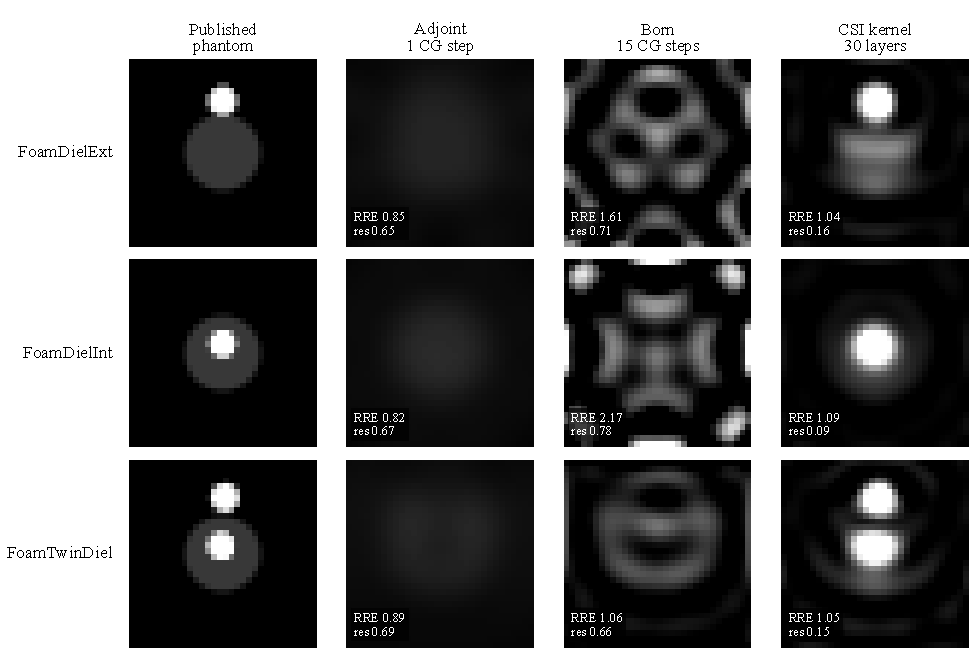
\includegraphics[width=\linewidth]{figures/fig_fresnel_recon.pdf}
\caption{$3\,\mathrm{GHz}$ 处的实测数据重建，每个公开体模一行。列是在同一实测场、标定常数、投影盒与 CG 求解上计算的算法阶梯：公开体模、伴随（一次 CG 步）、Born（入射场上 $15$ 次 CG 步）以及 $30$-层对比度源核。所有面板共享一个灰度 $[0,1]$，因此伴随列并非空，而是被强烈压缩（$\max|\chi|\le\numv{\NumFrBaseDsmPeakHi}$）。角值为相对误差与无标签数据残差。}
\label{fig:fresnelrecon}
\end{figure}

表~\ref{tab:fresnelrecon} 与图~\ref{fig:fresnelrecon} 报告结果。恢复的残差 $r_{\mathrm{net}}$ 落在 $0.07$ 与 $0.50$ 之间，对照模型到仪器的地板 $r_{\mathrm{true}}$ 在 $0.09$ 与 $0.12$ 之间；在九个实例中的两个（FoamDielInt 在 $3$ 与 $4\,\mathrm{GHz}$）处，恢复的残差\emph{低于}公开体模自身的拟合，而在最坏情况（FoamTwinDiel 在 $4\,\mathrm{GHz}$）处它在约 $4.7$ 倍于该地板之内。图像定量确认了这一点：单圆柱与双圆柱被定位，明亮塑料内含物与较弱泡沫基体由对比度区分，最坏情况是最高频率处的三圆柱双体模。整个展开中对比度源停留在 $\max\|w\|_\infty\in[0.04,0.09]$，且 $\max|\chi|$ 达到上盒边 $2.5$，在那里塑料圆柱饱和盒子。先验弱散射假设 $\beta_0=\chi_{\max}\norm{\mathbf{G}_b}_2<1$ 在此 $2\lambda$ 域上\emph{不}成立，如第~\ref{sec:fresnel} 节已报告；因此此处观测到的有界性是被实测展开轨迹的\emph{实测}有界性，而非场子系统收缩证书的后果。投影正是把该实测有界性转换为硬盒的东西；在测试实例中去掉投影本身在视界内并不产生发散，因此观测到的有界性本身并不是投影必要的证据。

图~\ref{fig:fresnelrecon} 中的阶梯是此图早先版本无法支持的、且不奉承内核的检查。伴随图像在三次重建中具有最小的相对误差（$\numv{\NumFrBaseDsmRreLo}$--$\numv{\NumFrBaseDsmRreHi}$），而 $30$-层核具有最大的（$\numv{\NumFrKernRreLo}$--$\numv{\NumFrKernRreHi}$）；顺序在无标签数据残差上反转（$\numv{\NumFrBaseDsmResLo}$--$\numv{\NumFrBaseDsmResHi}$ 对伴随，对照 $\numv{\NumFrKernResLo}$--$\numv{\NumFrKernResHi}$ 对核），且在图像本身上反转，因为伴随对比度峰值在 $\numv{\NumFrBaseDsmPeakHi}$，对照盒边 $2.5$。逐像素 $\ell_2$ 度量奖赏一个被压缩的图像，这正是使图~\ref{fig:images} 约束臂成为较大数字的同一机制；残差是表明一幅图像是否在解释测量的量。两个线性化求解把这一行为夹在中间（$\numv{\NumFrBaseBornRreLo}$--$\numv{\NumFrBaseBornRreHi}$，残差高至 $\numv{\NumFrBaseBornResHi}$），因此把核列与 Born 列分开的是非线性迭代而非线性求解。一个否定结果也属于此处：在 $3\,\mathrm{GHz}$ 处，步长搜索对三个体模都返回正则对 $(\alpha,\gamma)=(0.5,0.5)$，因此核列\emph{就是}存档重建，且搜索在这些实测情况下未添加任何东西；我们报告这而非重调它。

我们还尝试了训练修正网络的直接零样本迁移。选择每视角八个视角与两百四十一个接收机中的三十二个，使输入通道计数与训练检查点对齐，因此状态字典精确加载。然而被迁移的运行坍缩到近零图像：在九个实例中 $\max|\chi|$ 都保持在 $0.13$ 以下，且无标签残差保持在近一处，因为训练特征映射期望合成点扩散与固定的接收机 Green 块，而实测几何具有每视角弧与不同的场归一化。坍缩值本身落在盒内；上夹紧不活跃，因此有界性在此实例中是空真而非由投影强制。这不是有界性证书的失败——它只依赖于 $\mathbf{G}_b,\mathbf{G}_s$ 与投影集而非修正权重；它是证书跨几何迁移而训练特征映射不迁移的证据。

\section{讨论与局限}\label{sec:lim}
我们的结果认证的是一个\emph{机制}，而非每个机制，且若干发现是否定性的。
(i) 逐层欧氏收缩在 $\alpha>\alpha_c$ 上由命题~\ref{prop:imposs} 不可能，阈值 $\alpha_c=(\theta\mathcal{E})^{-1}$ 在此实测为 $\numv{\NumAlphaC}$；而将由收缩推出的几何界——漂移半径 $\bar\epsilon/(1-\rho_\chi)$ 与噪声增益 $\Lambda/(1-\rho)$——因此是\emph{条件性的}，且假设未被我们的实测全部 discharged：$\sigma_{\max}=\numv{\NumPhysSigma}>1$ 成立，而 $\rho_\chi<1$ 在无约束臂中被否定、在约束臂中未被决定。我们转而报告实测量，且认为在不带其假设的情况下引用任一半径都是对本理论所证明内容的歪曲。
(ii) 先验场证书要求 $\beta_0=\chi_{\max}\norm{\mathbf{G}_b}_2<1$。在其外（强散射体）投影与精确刻画仍有意义，但收缩论断失去其假设。
(iii) 振幅与斜率预算在我们的设定下不改善实测精度或实测噪声鲁棒性；它们的贡献在于每个训练网络都携带显式、可重算的常数。因此我们不以精度改进来报告预算化架构。
(iv) 投影对有界性是承重元素，但只是\emph{非扩张}而非收缩：它自身不能创造不动点，只能阻止逃逸并提供已知常数。物理核在场变量上不收缩（强对比度）的网络将需要注记~\ref{rem:averaged} 的平均算子构造，并付出命题~\ref{prop:tri} 所确认的精度代价。
(v) 我们的消融也显示了基于消融推理的局限：一个去掉投影重训练的网络在 $800$ 层处看着不错，只有表~\ref{tab:abl2} 报告的冻结权重测试才揭示同一权重在去掉投影时坍缩。联合重训练后观测到的有界性并不是防护栏不必要的证据。
(vi) 实验是二维且中等规模的。然而理论是维度无关的，且表~\ref{tab:cert} 中每个被认证量都从实践者可针对任何网格、孔径或对比度分布重算的量计算——\emph{前提是那些认证假设在该工作点处被检查}，因为在我们的工作点它们并非全部满足：定理~\ref{thm:field} 场证书的 $\beta_0<1$、定理~\ref{thm:bounded} 不变性的容许对比度盒，以及 \eqref{eq:budgets} 修正 $H_k$ 的振幅/斜率预算。证书只与那次检查一样好。两个建模限制也位于所述理论之外。首先，对比度取为\emph{实且非负}，正如对被动无损耗介质，这恰是使 $\Pi_{[0,\chi_{\max}]}$ 成为容许物理先验的原因；对有损耗或active 介质，对比度为复数，投影没有对应的写法；一个类似的证书将需要一个带有自身常数的复容许集。其次，$\beta_0$ 依赖于 $\norm{\mathbf{G}_b}_2$ 因而依赖于离散化，因此场证书是针对实际使用的离散化而非连续问题陈述的。第~\ref{sec:grid} 节在 $64\times64$ 与 $128\times128$ 单元上的重算保持 $\beta_0<1$ 且把算子级量移动不到 $1\%$，但证书仍是离散化层级的对象，这正是论断的范围。
(vii) 已学习修正改善条件数与速度而非信息内容：噪声敏感度地板由测量算子设定。
(viii) 不可能性命题按工作点陈述：$\alpha_c$ 依赖于 $\mathcal{E}=\max_r\norm{E_{\cdot,r}}_2$，它在测试集上沿展开变化。我们已在用于表~\ref{tab:cert} 的实测工作点处报告它，并在图~\ref{fig:alphac} 中扫描它；一个无分布的版本将需要对场集中的下界，我们没有也不声称有。
(ix) 第~\ref{sec:exp} 节的精度比较是对阻尼交替不动点迭代、在匹配逐层代价下的\emph{迭代次数}比较，而非对既定经典求解器的墙钟比较。我们量化了已学习模块的逐层附加费（$1{+}\numv{\NumCostLayerOverhead}$，中位数墙钟，在批大小 $16$ 的生产形状上比经典层高 $\numv{\NumCostLayerOverheadPct}\%$），以使读者能折扣迭代缩减，但我们不声称 $12\times$ 迭代缩减转化为 $12\times$ 墙钟缩减。我们现在还运行了两个更强的经典参照——对比度源反演与子空间优化方法，它们也保持在展开网络之上：在匹配深度处对 SOM 的边距为 $\numv{\NumSomMargKEight}$，而最佳对最佳边距 $\numv{\NumSomMargBest}$ 落在重跑地板之内。因此比较不是弱基线假象，且也不作为匹配预算下的胜利被声称。
(x) 对比度步由固定 $n_{\mathrm{cg}}=\numv{\NumNCg}$ 步共轭梯度循环而非收敛求解求值。被认证的块 $C$ 与 $D$ 是闭式且与求解器无关，因此不可能性与有界性论断不受影响；但对比度路径 Jacobian 块 $A$、$B$ 与全层范数\emph{确实}依赖于求解器分辨率，且我们在已实现与收敛两种设定下都报告它们而非引用一个，并带有固定效应的方向导数控制与测量该效应的系统性 $n_{\mathrm{cg}}$ 扫描。读者重算的任何对比度路径量都应在匹配的求解器分辨率下比较。
(xi) 本研究是理论与合成二维 TM 数据上的仿真，由第~\ref{sec:fresnel} 节的算子级 Fresnel 重算与第~\ref{sec:fresnelrecon} 节的实测场重建扩展。算子级重算在公开几何的一个频率与一个目标上使用我们自有的正向解；实测重建使用三个介质体模在三个 ROI 内频率上的真实散射场，但运行不带训练修正权重的经典层结构，因为那些权重期望训练点扩散。在九个实测实例中的两个，恢复的残差达到或低于公开体模自身的拟合；其余实例在该地板的大约 $4$ 倍之内。训练权重的直接零样本迁移被尝试并坍缩到近零图像，因此几何自适应的迁移仍是未来工作。

(xii) 第~\ref{sec:exp} 节的实证泛化结论来自单一 $32\times32$ 网格上 $\chi\in[0.25,0.5]$ 的合成数据。跨对比度边界在第~\ref{sec:contrast} 节测量、跨几何行为在第~\ref{sec:geom} 节测量：场子系统证书 $\beta_0<1$ 只在 $\chi_{\max}=\numv{\NumMaxChiBox}$ 处成立，并在每个被抬高的上限处失效，在那里只有投影保持状态有界，且估计由截断而非不稳定性退化；在四个结构上不同的几何族上，重建误差停留在一个温和带内，且投影有界性在深度 $100$ 处无条件成立。共享的对比度范围与网格分辨率仍是范围限制；第~\ref{sec:fresnelrecon} 节的实测场重建使用不带训练权重的经典层。

\section{结论}
我们着手陈述可以为一个展开式 Born/对比度源网络保证什么，而答案有着确定的形状。层 Jacobian 的 $\chi\!\to\!w$ 块恰为 $\theta\alpha\,\mathrm{diag}(E)$，因此对于 $\alpha>\alpha_c=(\theta\mathcal{E})^{-1}$ 与\emph{每个}已学习修正，复合层被证明为非收缩的，且障碍位于一个仅施加于对比度的修正所不能触及的通道。这是架构的性质，而非数据、损失或训练调度的性质。

存活下来的是逐层的。一个场子系统收缩 $\beta_0=\chi_{\max}\norm{\mathbf{G}_b}_2$ 在它成立的所有步长处都成立；一个不变紧集在非扩张物理先验投影下被认证用于任意深度；有限深度噪声传播被精确刻画，包括几何级数所遗漏的非正规因子；且两条几何性论断被标记为条件性，因为它们的假设在我们的工作点处未被 discharged。检查有顺序：训练前在实际离散化上的 $\beta_0$、训练期间的投影与主干边界，以及每个新工作点处的重测 $(\sigma_{\max}(J),\rho,M_J,\Lambda)$。常数的代价是被实测而非被论证的：在匹配深度处，约束族在测试集相对重建误差上比无约束族差 $\numv{\NumPriceDelta}$，而该差距买来的是一个可重算的常数，而非一个可被假设的速率。

范围限制是结果的一部分。每个证书都条件于离散化、孔径、对比度盒与工作点；在公开 Fresnel 几何上 $\beta_0=\numv{\NumFresnelBeta}$，因此那里没有可用的先验场证书，有界性是所剩之物；且漂移半径所需的 $\chi$-映射 Lipschitz 常数既未被我们可测的代理否定也未证实，这正是该半径保持条件性的原因。此处没有任何东西证明一个训练网络收敛：没有不动点被显示存在、唯一或吸引，且不声称无条件的噪声增益；两条被证明的论断涉及场子系统与不变集，它们是全部先验内容。把证书带到其场步并非 Born/对比度源的核，并 discharge $\chi$-映射假设而非界定它，是边界现在移动的两条方向。

\section*{致谢}
不适用。

\section*{基金资助}
本研究由河南省科技攻关项目资助，项目编号 262102210030 与 242102321138。

\section*{作者贡献}
作者确认对本文的贡献如下：概念化，王龙江；方法论，王龙江；软件，王国强；验证，王国强与史念锋；形式分析，王龙江；调查，王国强与史念锋；资源，史念锋；数据整理，王国强；初稿撰写，王龙江；审阅与编辑，王龙江与王国强；可视化，王国强；监督，王龙江；项目管理，王龙江；资金获取，王龙江。所有作者审阅并批准了稿件的最终版本。

\section*{数据与材料可用性}
支持本研究发现的代码与数值日志在 GitHub 仓库 \url{https://github.com/jiumi01/unrolled-inverse-scattering}（tag v1.1）公开可用。实测的 Institut Fresnel 数据集可从 Institut Fresnel 网站获取。

\section*{伦理审批}
不适用。本研究不涉及人类参与者、人体组织或动物；第~\ref{sec:fresnelrecon} 节使用的实测场是一个公开散射数据库。

\section*{利益冲突}
作者声明无利益冲突。

\clearpage
\section*{缩写}
下列缩写用于本手稿：
\begin{center}
\footnotesize
\begin{tabular}{@{}ll@{}}
2-D & 二维（two-dimensional）\\
CG & 共轭梯度（conjugate gradient）\\
CIE & 压缩积分方程（contraction / compressed integral equation）\\
CSI & 对比度源反演（contrast source inversion）\\
GMRES & 广义最小残差法（generalised minimal residual method）\\
ISP & 逆散射问题（inverse scattering problem）\\
LS & Lippmann--Schwinger\\
MoM & 矩量法（method of moments）\\
NBIM & 神经 Born 迭代法（Neural Born Iterative Method）\\
RRE & 相对重建误差（relative reconstruction error）\\
SNR & 信噪比（signal-to-noise ratio）\\
SOM & 基于子空间的优化方法（subspace-based optimization method）\\
TM & 横磁（transverse magnetic）
\end{tabular}
\end{center}

\section*{参考文献}
\begin{thebibliography}{99}
\bibitem{born_lit}
Habashy TM, Groom RW, Spies BR. Beyond the Born and Rytov approximations: A nonlinear approach to electromagnetic scattering. J Geophys Res. 1993;98(B2):1759--1775.
\bibitem{csi_lit}
van den Berg PM, Kleinman RE. A contrast source inversion method. Inverse Probl. 1997;13(6):1607--1620.
\bibitem{som_lit}
Chen X. Subspace-based optimization method for solving inverse-scattering problems. IEEE Trans Geosci Remote Sens. 2010;48(1):42--49.
\bibitem{somnet}
Liu Y, Zhao H, Song R, Chen X, Li C, Chen X. SOM-Net: Unrolling the subspace-based optimization for solving full-wave inverse scattering problems. IEEE Trans Geosci Remote Sens. 2022;60:2007715.
\bibitem{unrolledcnn}
Zhang Y, Lambert M, Fraysse A, Lesselier D. Unrolled convolutional neural network for full-wave inverse scattering. IEEE Trans Antennas Propag. 2023;71(1):947--956.
\bibitem{neuralbim}
Shan T, Lin Z, Song X, Li M, Yang F, Xu S. Neural Born iterative method for solving inverse scattering problems: 2D cases. IEEE Trans Antennas Propag. 2023;71(1):818--829.
\bibitem{deepnis}
Li L, Wang LG, Teixeira FL, Liu C, Nehorai A, Cui TJ. DeepNIS: Deep neural network for nonlinear electromagnetic inverse scattering. IEEE Trans Antennas Propag. 2019;67(3):1819--1825.
\bibitem{mfneuralbim}
Liu D, Shan T, Li M, Yang F, Xu S. Multi-frequency neural Born iterative method for solving 2-D inverse scattering problems. IEEE Trans Comput Imaging. 2025;11:1243--1257.
\bibitem{ciesomnet}
Xu K, et al. Physically unrolling network under contraction integral equation for limited-aperture inverse scattering problem. IEEE Trans Antennas Propag. 2023;71(11):9130--9135.
\bibitem{kernelunroll}
Li X, Zhang T, Bi D, Peng L, Xie Y. Kernelized deep unfolding network with joint physical constraints for electromagnetic inverse scattering imaging. IEEE Trans Antennas Propag. 2026;74(2):1707--1722.
\bibitem{li2019cnn}
Li L, Wang LG, Teixeira FL. Performance analysis and dynamic evolution of deep convolutional neural network for electromagnetic inverse scattering. IEEE Antennas Wireless Propag Lett. 2019;18(11):2259--2263.
\bibitem{lista}
Gregor K, LeCun Y. Learning fast approximations of sparse coding. In: Proc ICML; 2010. p. 399--406.
\bibitem{listacp}
Chen X, Liu J, Wang Z, Yin W. Theoretical linear convergence of unfolded ISTA and its practical weights and thresholds. In: Proc NeurIPS; 2018.
\bibitem{alista}
Liu J, Chen X, Wang Z, Yin W. ALISTA: Analytic weights are as good as learned weights in LISTA. In: Proc ICLR; 2019.
\bibitem{cui_reg}
Cui ZX, Zhu Q, Cheng J, Zhang B, Liang D. Deep unfolding as iterative regularization for imaging inverse problems. Inverse Probl. 2024;40(2):025011.
\bibitem{sherry_nonexp}
Sherry F, Celledoni E, Ehrhardt MJ, Murari D, Owren B, Sch\"onlieb CB. Designing stable neural networks using convex analysis and ODEs. Physica D. 2024;463:134159.
\bibitem{mondeq}
Winston E, Kolter JZ. Monotone operator equilibrium networks. In: Proc NeurIPS; 2020.
\bibitem{algomapping}
Tay DB. On iterative algorithms with different mapping in each iteration. Algorithms. 2026;19(6):470.
\bibitem{mukherjee2023}
Mukherjee S, Hauptmann A, \"Oktem O, Pereyra M, Sch\"onlieb CB. Learned reconstruction methods with convergence guarantees: A survey of concepts and applications. IEEE Signal Process Mag. 2023;40(1):164--182.
\bibitem{monga_survey}
Monga V, Li Y, Eldar YC. Algorithm unrolling: Interpretable, efficient deep learning for signal and image processing. IEEE Signal Process Mag. 2021;38(2):18--44.
\bibitem{convergentborn}
Kleinman RE, Roach GF, van den Berg PM. Convergent Born series for large refractive indices. J Opt Soc Am A. 1990;7(5):890--897.
\bibitem{cie_lit}
Isernia T, Crocco L, D'Urso M. New tools and series for forward and inverse scattering problems in lossy media. IEEE Geosci Remote Sens Lett. 2004;1(4):327--331.
\bibitem{kleinvandenberg}
Kleinman RE, van den Berg PM. Iterative methods for solving integral equations. Prog Electromagn Res. 1991;5:67--102.
\bibitem{slaney}
Slaney M, Kak AC, Larsen LE. Limitations of imaging with first-order diffraction tomography. IEEE Trans Microw Theory Tech. 1984;32(8):860--874.
\bibitem{devalle2023}
de Valle C, Centofanti E, Chouzenoux E, Pesquet JC. Stability of unfolded forward-backward to perturbations in observed data. In: Proc 31st Eur Signal Process Conf (EUSIPCO); 2023. p. 865--869.
\bibitem{fresnel_db}
Belkebir K, Saillard M. Special section: Testing inversion algorithms against experimental data. Inverse Probl. 2001;17(6):1565--1571; Geffrin JM, Sabouroux P, Eyraud C. Free space experimental scattering database continuation: experimental set-up and measurement precision. Inverse Probl. 2005;21(6):S117--S130.
\end{thebibliography}

\end{document}
